% Elements from default .Rmd template
% Options for packages loaded elsewhere
\PassOptionsToPackage{unicode}{hyperref}
\PassOptionsToPackage{hyphens}{url}

%%%%%%%%%%%%%%%%%%%%%%%%%%%%%%%%%%%%%%%%%%%%%%%%%%%%%%%%%%%%
%%% ELIFE ARTICLE TEMPLATE documentclass
%%%%%%%%%%%%%%%%%%%%%%%%%%%%%%%%%%%%%%%%%%%%%%%%%%%%%%%%%%%%
\documentclass[9pt,lineno]{elife}


% Elements from default .Rmd template again
\usepackage{amsmath,amssymb}
\usepackage{lmodern}
\usepackage{iftex}
\ifPDFTeX
  \usepackage[T1]{fontenc}
  \usepackage[utf8]{inputenc}
  \usepackage{textcomp} % provide euro and other symbols
\else % if luatex or xetex
  \usepackage{unicode-math}
  \defaultfontfeatures{Scale=MatchLowercase}
  \defaultfontfeatures[\rmfamily]{Ligatures=TeX,Scale=1}
\fi
% Use upquote if available, for straight quotes in verbatim environments
\IfFileExists{upquote.sty}{\usepackage{upquote}}{}
\IfFileExists{microtype.sty}{% use microtype if available
  \usepackage[]{microtype}
  \UseMicrotypeSet[protrusion]{basicmath} % disable protrusion for tt fonts
}{}
\makeatletter
\@ifundefined{KOMAClassName}{% if non-KOMA class
  \IfFileExists{parskip.sty}{%
    \usepackage{parskip}
  }{% else
    \setlength{\parindent}{0pt}
    \setlength{\parskip}{6pt plus 2pt minus 1pt}}
}{% if KOMA class
  \KOMAoptions{parskip=half}}
\makeatother
\usepackage{xcolor}
\IfFileExists{xurl.sty}{\usepackage{xurl}}{} % add URL line breaks if available
\IfFileExists{bookmark.sty}{\usepackage{bookmark}}{\usepackage{hyperref}}
\hypersetup{
  pdftitle={A comprehensive proteomic and bioinformatics analysis of human spinal cord injury plasma identifies proteins associated with the complement cascade as potential prognostic indicators of neurological outcome},
  pdfkeywords={Spinal cord injury, biomarker, proteomics, complement},
  hidelinks,
  pdfcreator={LaTeX via pandoc}}
\urlstyle{same} % disable monospaced font for URLs
\usepackage{longtable,booktabs,array}
\usepackage{calc} % for calculating minipage widths
% Correct order of tables after \paragraph or \subparagraph
\usepackage{etoolbox}
\makeatletter
\patchcmd\longtable{\par}{\if@noskipsec\mbox{}\fi\par}{}{}
\makeatother
% Allow footnotes in longtable head/foot
\IfFileExists{footnotehyper.sty}{\usepackage{footnotehyper}}{\usepackage{footnote}}
\makesavenoteenv{longtable}
\usepackage{graphicx}
\makeatletter
\def\maxwidth{\ifdim\Gin@nat@width>\linewidth\linewidth\else\Gin@nat@width\fi}
\def\maxheight{\ifdim\Gin@nat@height>\textheight\textheight\else\Gin@nat@height\fi}
\makeatother
% Scale images if necessary, so that they will not overflow the page
% margins by default, and it is still possible to overwrite the defaults
% using explicit options in \includegraphics[width, height, ...]{}
\setkeys{Gin}{width=\maxwidth,height=\maxheight,keepaspectratio}
% Set default figure placement to htbp
\makeatletter
\def\fps@figure{htbp}
\makeatother
\setlength{\emergencystretch}{3em} % prevent overfull lines
\providecommand{\tightlist}{%
  \setlength{\itemsep}{0pt}\setlength{\parskip}{0pt}}
\setcounter{secnumdepth}{5}
\newlength{\cslhangindent}
\setlength{\cslhangindent}{1.5em}
\newlength{\csllabelwidth}
\setlength{\csllabelwidth}{3em}
\newlength{\cslentryspacingunit} % times entry-spacing
\setlength{\cslentryspacingunit}{\parskip}
\newenvironment{CSLReferences}[2] % #1 hanging-ident, #2 entry spacing
 {% don't indent paragraphs
  \setlength{\parindent}{0pt}
  % turn on hanging indent if param 1 is 1
  \ifodd #1
  \let\oldpar\par
  \def\par{\hangindent=\cslhangindent\oldpar}
  \fi
  % set entry spacing
  \setlength{\parskip}{#2\cslentryspacingunit}
 }%
 {}
\usepackage{calc}
\newcommand{\CSLBlock}[1]{#1\hfill\break}
\newcommand{\CSLLeftMargin}[1]{\parbox[t]{\csllabelwidth}{#1}}
\newcommand{\CSLRightInline}[1]{\parbox[t]{\linewidth - \csllabelwidth}{#1}\break}
\newcommand{\CSLIndent}[1]{\hspace{\cslhangindent}#1}
\usepackage{pdflscape}
\newcommand{\blandscape}{\begin{landscape}}
\newcommand{\elandscape}{\end{landscape}}
\usepackage{float} \floatplacement{figure}{H}
\newcommand{\beginsupplement}{\setcounter{table}{0}  \renewcommand{\thetable}{S\arabic{table}} \setcounter{figure}{0} \renewcommand{\thefigure}{S\arabic{figure}}}
\usepackage{booktabs}
\usepackage{longtable}
\usepackage{array}
\usepackage{multirow}
\usepackage{wrapfig}
\usepackage{float}
\usepackage{colortbl}
\usepackage{pdflscape}
\usepackage{tabu}
\usepackage{threeparttable}
\usepackage{threeparttablex}
\usepackage[normalem]{ulem}
\usepackage{makecell}
\usepackage{xcolor}
\ifLuaTeX
  \usepackage{selnolig}  % disable illegal ligatures
\fi

\title{A comprehensive proteomic and bioinformatics analysis of human spinal cord injury plasma identifies proteins associated with the complement cascade as potential prognostic indicators of neurological outcome}
\author{}
\date{2022-05-10 16:47:11}

%%%%%%%%%%%%%%%%%%%%%%%%%%%%%%%%%%%%%%%%%%%%%%%%%%%%%%%%%%%%
%%% ELIFE ARTICLE TEMPLATE again
%%%%%%%%%%%%%%%%%%%%%%%%%%%%%%%%%%%%%%%%%%%%%%%%%%%%%%%%%%%%
% Use the onehalfspacing option for 1.5 line spacing
% Use the doublespacing option for 2.0 line spacing
% Please note that these options may affect formatting.
% Additionally, the use of the \newcommand function should be limited.

\usepackage{lipsum} % Required to insert dummy text
\usepackage[version=4]{mhchem}
\usepackage{siunitx}
\DeclareSIUnit\Molar{M}

%%%%%%%%%%%%%%%%%%%%%%%%%%%%%%%%%%%%%%%%%%%%%%%%%%%%%%%%%%%%
%%% ARTICLE SETUP
%%%%%%%%%%%%%%%%%%%%%%%%%%%%%%%%%%%%%%%%%%%%%%%%%%%%%%%%%%%%
% \title{This is the title}

% \author[1*]{Firstname Middlename Surname}
% \author[1,2\authfn{1}\authfn{3}]{Firstname Middlename Familyname}
% \author[2\authfn{1}\authfn{4}]{Firstname Initials Surname}
% \author[2*]{Firstname Surname}
% \affil[1]{Institution 1}
% \affil[2]{Institution 2}

% \corr{email1@example.com}{FMS}
% \corr{email2@example.com}{FS}

% \contrib[\authfn{1}]{These authors contributed equally to this work}
% \contrib[\authfn{2}]{These authors also contributed equally to this work}

% \presentadd[\authfn{3}]{Department, Institute, Country}
% \presentadd[\authfn{4}]{Department, Institute, Country}
% \presentadd[\authfn{5}]{eLife Sciences editorial Office, eLife Sciences, Cambridge, United Kingdom}

%%%%%%%%%%%%%%%%%%%%%%%%%%%%%%%%%%%%%%%%%%%%%%%%%%%%%%%%%%%%
%%% ARTICLE START
%%%%%%%%%%%%%%%%%%%%%%%%%%%%%%%%%%%%%%%%%%%%%%%%%%%%%%%%%%%%

\begin{document}

\maketitle

\hypertarget{abstract}{%
\section{Abstract}\label{abstract}}

Introduction

Spinal Cord Injury (SCI) is a major cause of disability, with complications post-injury often leading to life-long health issues with need of extensive treatment. Neurological outcome post-SCI can be variable and difficult to predict, particularly in incomplete injured patients. The identification of specific SCI biomarkers in blood, may be able to improve prognostics in the field. This study has utilised proteomic and bioinformatics methodologies to investigate differentially expressed proteins in plasma samples across human SCI cohorts with the aim of identifying prognostic biomarkers and biological pathway alterations that relate to neurological outcome.

Methods and Materials

Blood samples were taken, following informed consent, from ASIA impairment scale (AIS) grade C ``Improvers'' (AIS grade improvement) and ``Non-Improvers'' (No AIS change), and AIS grade A and D at \textless2 weeks (``Acute'') and approx. 3 months (``Sub-acute'') post-injury. The total protein concentration from each sample was extracted, with pooled samples being labelled and non-pooled samples treated with ProteoMiner™ beads. Samples were then analysed using two 4-plex isobaric tag for relative and absolute quantification (iTRAQ) analyses and a label-free experiment for comparison, before quantifying with mass spectrometry. Proteomic datasets were analysed using \textbf{bioinformatics\ldots{}}

Proteins of interest identified from this analysis were further validated by enzyme-linked immunosorbent assay (ELISA).
OpenMS (version 2.6.0) was used to process the raw spectra data.
R (version 4.1.4) and in particular, the R packages MSstats (version 4.0.1), STRINGdb (version 2.4.2) and pathview (version 1.32.0) were used for downstream analysis.

Results

The data demonstrated proteomic differences between the cohorts, with the results from the iTRAQ approach supporting those of the label-free analysis. A total of 79 and 87 differentially abundant proteins across AIS and longitudinal groups were identified from the iTRAQ and label-free analyses, respectively. Alpha-2-macroglobulin (A2M), retinol binding protein 4 (RBP4), serum amyloid A1 (SAA1), Peroxiredoxin 2, alipoprotein A1 (ApoA1) and several immunoglobulins were identified as biologically relevant and differentially abundant, with potential as individual prognostic biomarkers of neurological outcome. Bioinformatics analyses revealed that the majority of differentially abundant proteins were components of the complement cascade and most interacted directly with the liver.

Conclusions

Many of the proteins of interest identified using proteomics were detected only in a single group and therefore have potential as a binary (present or absent) biomarkers. Additional investigations into the chronology of these proteins, and their levels in other tissues (cerebrospinal fluid in particular) are needed to better understand the underlying pathophysiology, including any potentially modifiable targets. \textbf{The complement cascasde was confirmed using pathway analysis as\ldots{}}

\hypertarget{introduction}{%
\section{Introduction}\label{introduction}}

Spinal cord injury (SCI) is the transient or permanent loss of normal spinal sensory, motor or autonomic function, and is a major cause of disability. Globally, SCI affects around 500,000 people each year and is most commonly the result of road traffic accidents or falls.(Crozier-Shaw, Denton, and Morris 2020)
Patients typically require extensive medical, rehabilitative and social care at high financial cost to healthcare providers. The lifetime cost of care in the UK is estimated to be £1.12 million (mean value) per SCI, with the total cost of SCI in the UK to the NHS being £1.43 billion in 2016.(McDaid et al. 2019)
Individuals with SCI show markedly higher rates of mental illness relative to the general population.(Furlan, Gulasingam, and Craven 2017)
Complications arising post-SCI can be long-lasting and often include pain, spasticity and cardiovascular disease, where the systemic inflammatory response that follows SCI can frequently result in organ complications, particularly in the liver and kidneys.(Gris, Hamilton, and Weaver 2008; X. Sun et al. 2016)

The recovery of neurological function post-SCI is highly variable, requiring any clinical trials to have an impractically large sample size to prove efficacy, hence the translation of novel efficacious therapies is challenging and expensive.(Spiess et al. 2009)
Being able to more accurately predict patient outcomes would aid clinical decisions and facilitate future clinical trials. Therefore, novel biomarkers that allow for stratification of injury severity and capacity for neurological recovery would be of high value to the field.

Biomarkers studies in SCI often investigate protein changes in cerebral spinal fluid (CSF) as the closer proximity of this medium is thought to be more reflective of the parenchymal injury.(Brian K. Kwon et al. 2019; Hulme et al. 2017)
Whilst this makes CSF potentially more informative for elucidating the pathology of SCI, the repeated use of CSF for routine analysis presents challenges in clinical care due to the risk and expense associated with the invasiveness of the collection procedure. In contrast, systemic biomarkers measurable in the blood represent a source of information that can be accessed and interpreted both a lower cost and risk. Studies of traumatic brain injury have demonstrated that protein markers identified in CSF are also detectable in both plasma and serum.(Wang et al. 2018) More recently, circulating white blood cell populations have also been identified as potential SCI injury biomarkers, with a 2021 study showing that elevated levels of neutrophils were associated with no AIS grade conversion, while conversely an increase in lymphocytes during the first week post-SCI were associated with an AIS grade improvement.

A number of individual proteins have been shown to be altered in the bloods post-SCI, including multiple interleukins (IL), tumour necrosis factor alpha (TNF-\(\alpha\)) and C-reactive protein (CRP).(Segal et al. 1997; Hayes et al. 2002; Frost et al. 2005)

Further, changes in inflammatory marker levels detected in acute SCI patients were found to be mirrored in donor-matched blood and CSF, albeit at lower absolute concentrations systemically.(Brian K. Kwon et al. 2010)

Previously, we have shown that routinely collected blood measures associated with liver function and inflammation added predictive value to AIS motor and sensor outcomes at discharge and 12-months post-injury.(Bernardo Harrington et al. 2020; Brown et al. 2019) The current study uses an unbiased shotgun proteomic approach to investigate differentially expressed proteins in SCI patients, coupled with bioinformatics pathway and network analyses.

\hypertarget{methods-and-materials}{%
\section{Methods and Materials}\label{methods-and-materials}}

\begin{longtable}[t]{lll}
\caption{\label{tab:patient-demo-chap3}Patient demographics. ± denotes interquartile range}\\
\toprule
 & n & Percent\\
\midrule
\endfirsthead
\caption[]{\label{tab:patient-demo-chap3}Patient demographics. ± denotes interquartile range \textit{(continued)}}\\
\toprule
 & n & Percent\\
\midrule
\endhead

\endfoot
\bottomrule
\endlastfoot
\addlinespace[0.3em]
\multicolumn{3}{l}{\textbf{Polytrauma}}\\
\hspace{1em}Yes & 16 & 41\\
\hspace{1em}No & 23 & 59\\
\addlinespace[0.3em]
\multicolumn{3}{l}{\textbf{Gender}}\\
\hspace{1em}F & 13 & 33\\
\hspace{1em}M & 26 & 67\\
\addlinespace[0.3em]
\multicolumn{3}{l}{\textbf{Diabetes}}\\
\hspace{1em}Yes & 7 & 18\\
\hspace{1em}No & 32 & 82\\
\addlinespace[0.3em]
\multicolumn{3}{l}{\textbf{Neurological level}}\\
\hspace{1em}C & 26 & 67\\
\hspace{1em}L & 4 & 10\\
\hspace{1em}T & 9 & 23\\
\addlinespace[0.3em]
\multicolumn{3}{l}{\textbf{AIS change}}\\
\hspace{1em}A & 11 & 28\\
\hspace{1em}C & 7 & 18\\
\hspace{1em}C->D & 10 & 26\\
\hspace{1em}D & 11 & 28\\
Age at injury 
(Median years±IQR) & 53±26 & -\\*
\end{longtable}

\hypertarget{patients}{%
\subsection{Patients}\label{patients}}

Blood samples were taken from SCI patients who had provided informed consent and in accordance to ethical provided by the National Research Ethics Service {[}NRES{]} Committee North West Liverpool East {[}11/NW/0876{]}. ``Improvers'' were defined as individuals who experienced an AIS grade improvement from admission to a year post-injury, whereas ``non-improvers'' were defined as patients who saw no change in AIS grade in the same period.

\hypertarget{plasma-collection-and-storage}{%
\subsection{Plasma collection and storage}\label{plasma-collection-and-storage}}

Plasma samples were collected within 2 weeks of injury (acute) and at approximately 3 months post-injury (subacute). Upon collection in EDTA (ethylenediaminetetraacetic acid) coated tubes samples were centrifuged at 600g for 15 minutes, to pellet erythrocytes and the resultant plasma fraction was aspirated and divided into aliquots for long-term storage in -80°C briefly and liquid nitrogen in the longer term.

\hypertarget{itraq-sample-prep}{%
\subsection{Sample preparation and analysis using iTRAQ proteomics}\label{itraq-sample-prep}}

Thawed plasma samples (\(2\mu l\)) each were diluted with distilled water (\(98\mu l\)). Total protein was quantified using a Pierce™ \(660 nm\) Protein Assay (Thermo Fisher Scientific, Hemel Hempstead, UK)(Stoscheck 1987).

In brief, \(10\mu l\) of the diluted sample was added to \(150\mu l\) of Thermo Pierce 660nm protein assay reagent in triplicate and the optical density was read at 660nm.

A total of \(100 mg\) of plasma protein was taken from each sample and pooled equally to form a patient test group.
For example, the AIS C improver group was pooled from 10 separate patient samples, 10mg of protein per patient.

The pooled plasma samples were then precipitated by incubation of the sample in 6 times the volume of chilled acetone for 1 hour at -20°C.
The samples were then centrifuged at 6,000G for 10 minutes at 4°C, and re-suspended in \(200\mu l\) of triethylammonium bicarbonate buffer.
Sequencing Grade Modified Trypsin (\(10\mu g/85\mu g\) of protein; Promega, Madison, WI, USA) was then added to the samples for overnight digestion at 37°C.
Proteins then underwent reduction and alkylation (according to the manufacturer's instructions; Applied Biosystems, Bleiswijk, The Netherlands).
Tryptic digests were labelled with iTRAQ tags (again according to the manufacturer's instructions for the iTRAQ kit), before being pooled into test groups and dried in a vacuum centrifuge.
The following tags were used for each group of patient samples 114 tag - acute improvers, 115 tag - sub-acute improvers, 116 tag - acute non-improvers and 117 tag - sub-acute non-improvers for run 1 and 114 tag - acute improvers, 115 tag - acute non-improvers, 116 tag - AIS grade A and 117 tag - AIS grade D for run 2.

\hypertarget{itraq-mass-spectrometry-analysis}{%
\paragraph{iTraq mass spectrometry analysis}\label{itraq-mass-spectrometry-analysis}}

The samples were analysed at the BSRC St.~Andrews University Mass Spectrometry and Proteomics Facility using methods previously described.

A total of 12 SCX fractions were analysed by nano-electrospray ionisation-liquid chromatography/tandem mass spectrometry (LC-MS/MS) using a TripleTOF 5600 tandem mass spectrometer (AB Sciex, Framingham, MA, USA) as described previously.(Fuller et al. 2015)

\textbf{SECTION TO BE REWRITTEN}
Each fraction (\(10 \mu l\)) was then analysed by nanoflow LC-ESI--MSMS. The peptides were separated using a nanoLC Ultra 2D plus loading pump and nanoLC AS-2 autosampler chromatography system (Eksigent, Redwood City, CA, USA), using a PepMap RSLC column (\(75\mu l\) x \(15 cm\)) and an Acclaim PepMap100 trap (\(100\mu m\) x \(2 cm\)) (ThermoFisher Scientific, Waltham, MA, USA).
After washing the peptides on the trap column for 20 minutes at \(5\mu L\) min\(^{-1}\), the trap was switched in line with the column and the peptides eluted with a gradient of increasing MeCN from 95\% buffer A (98\% H\textsubscript{2}O, 2\% MeCN, 0.1\% FA), 5\% buffer B (2\% H\textsubscript{2}O, 98\% MeCN, 0.1\% FA) to 65\% buffer A, 35\% buffer B over 60 minutes, then to 50\% buffer A, 50\% buffer B over a further 20 minutes, before increasing the concentration of buffer B to 95\% over a further 10 minutes.
The column was then washed with 95\% buffer B before re-equilibration in 95\% buffer A. A flow rate of \(300 nL\) min\(^{-1}\) was employed. The eluent was sprayed into a TripleTOF 5600 tandem mass spectrometer (ABSciex, Foster City, CA, USA), using a NANOSpray III source, and analyzed in Information Dependent Acquisition (IDA) mode, performing \(250 ms\) of MS followed by \(100 ms\) MSMS analyses on the 20 most intense peaks with a charge state of +2 to +5.
Parent (MS) ions were accepted with a mass tolerance of 50 mDa and MSMS was conducted with a rolling collision energy (CE) inclusive of preset iTRAQ CE adjustments.
Analyzed parent ions were then excluded from analysis for 13 s after 3 occurrences.

\hypertarget{label-free-sample-prep}{%
\subsubsection{Sample preparation and analysis using label-free proteomics}\label{label-free-sample-prep}}

No sample pooling was used, and so each of the 73 samples were maintained separately throughout protein equalisation, mass spectrometry, and label-free quantification steps.
Thus, protein abundance was quantified for each sample, whereupon mean protein abundance across experimental groups was calculated to assess protein changes.

To reduce the dynamic range of proteins, ProteoMiner™ beads (BioRad, Hemel Hempstead, UK) were used. Firstly, plasma was treated with 1 \(\mu g/mL\) of hyaluronidase. Digestion was confirmed with Coomassie stained 1D-SDS PAGE gel.
The supernatant was centrifuged through a 0.22 \(\mu m\) cellulose acetate membrane (Costar Spin-X, Corning, Tokyo, Japan) tube filter (5000\emph{g} for 15 minutes) to remove insoluble material.
Total protein was quantitated with a Pierce™ \(660 nm\) Protein Assay (Thermo Fisher Scientific, Hemel Hempstead, UK), whereupon 5 mg of total protein was applied to ProteoMiner™ beads, and processed as described previoulsly.(Stoscheck 1987)

\hypertarget{label-free-mass-spectrometry-analysis}{%
\paragraph{Label free mass spectrometry analysis}\label{label-free-mass-spectrometry-analysis}}

Tryptic peptides were subjected to LC-MC/MC via a 2-h gradient on a NanoAcquity™ ultraperformance LC (Waters, Manchester, UK) connected to a Q-Exactive Quadrupole-Orbitrap instrument (Thermo-Fisher Scientific Hemel Hempstead, UK) as described \textbf{previously}.

\textbf{REWRITE IN BRIEF}
The Q-Exactive was operated in a data dependent positive electrospray ionisation mode, automatically switching between full scan MS and MS/MS acquisition.
Survey full scan MS spectra (\emph{m/z} 300--2000) were acquired in the Orbitrap with 70,000 resolution (\emph{m/z} 200) following accumulation of ions to \(1\times 10^6\) target value based on the predictive automatic gain control values from the previous full scan.
Dynamic exclusion was set to 20s, the 10 most intense multiply charged ions (\(z \geq 2\)) were sequentially isolated and fragmented in the octopole collision cell by higher energy collisional dissociation (HCD), with a fixed injection time of 100ms and 35,000 resolution.
The following mass spectrometric conditions were used: spray voltage, 1.9kV, no sheath or axillary gas flow; normalised HCD collision energy 30\%; heated capillary temperature, 250°C.
MS/MS ion selection threshold was set to \(1\times 10^4\) count and 2Da isolation width was set.

\hypertarget{openms-chap3}{%
\subsubsection{iTraq OpenMS analysis}\label{openms-chap3}}

TripleTOF 5600 tandem mass spectrometer output files produced in the ABSciex proprietary \texttt{.wiff} file format were converted to an open file format, \texttt{.mzML} for analysis with OpenMS (version 2.6.0). The docker image of ProteoWizard version 3.0.20287 was used for conversion, and peak picking was applied on conversion (Chambers et al. 2012). OpenMS version 2.6.0 was used for further analysis.(Röst et al. 2016)
Unless otherwise stated, default arguments were used.
The 12 fraction files were merged and sorted by retention time.
A decoy database was generated with \texttt{DecoyDatabase} and the \texttt{-enzyme} flag set to \texttt{Trypsin}, the human reference proteome was taken from Uniprot (Proteome ID: UP000005640, downloaded: 2020-10-01), as was the \texttt{.fasta} for porcine trypsin (Entry: P00761, downloaded: 2020-10-01).(The UniProt Consortium 2021)

The \texttt{MSFGPlusAdapter} was used to run the search.
For the \texttt{-fixed\_modifications} ``Methylthio (C)'' and ``iTRAQ4plex (N-term)'' were passed due to the alkylating agent used in sample preperation and to account for the N-terminus modifications made by iTRAQ tags.
``Oxidation (M)'' was passed to \texttt{-variable\_modifications} to reflect the likely occurrence of methionine oxidation.
To reflect the instrument the following flags were also set: \texttt{-precursor\_mass\_tolerance\ 20\ -enzyme\ Trypsin/P\ -protocol\ iTRAQ\ -instrument\ high\_res}.

To annotate the search results \texttt{PeptideIndexer} and \texttt{PSMFeatureExtractor} were used.
For peptide level score estimation and filtering \texttt{PercolatorAdapter} was used with the following arguments: \texttt{-score\_type\ q-value\ -enzyme\ trypsinp}.
\texttt{IDFilter} was used to filter to a peptide score of 0.05 with \texttt{-score:pep\ 0.05}

\texttt{IsobaricAnalyzer} with \texttt{-type\ itraq4plex} was used with the merged \texttt{.mzML} files to assign protein-peptide identifications to features or consensus features with \texttt{IDMApper}.
The files for each run output by \texttt{IDMapper} were then merged with \texttt{FileMerger}.
Bayesian score estimation and protein inference was performed with \texttt{Epifany} and the following flags: \texttt{-greedy\_group\_resolution\ remove\_proteins\_wo\_evidence\ -algorithm:keep\_best\_PSM\_only\ false}
Decoys were removed and 0.05 FDR filtering was done via \texttt{IDFilter} with \texttt{-score:protgroup\ 0.05\ -remove\_decoys}.
Finally, \texttt{IDConflictResolver} was used to resolve ambiguous annotations of features with peptide identifications, before quantification with \texttt{ProteinQuantifier}.

\hypertarget{openms-label-free}{%
\subsubsection{Label free OpenMS analysis}\label{openms-label-free}}

For quantification, the raw spectra files were analysed via OpenMS (version 2.6.0) command line tools, with the workflow from the prior section (\ref{openms-chap3}) adapted to suit a label-free analysis.
The files were first converted from the proprietary .Raw format to the open .mzML standard with the \texttt{FileConverter} tool via the open-source \texttt{ThermoRawFileParser}.(Röst et al. 2016; Hulstaert et al. 2020)
Unless otherwise stated, default arguments were used throughout.

The decoy database generated in the prior section (iTRAQ OpenMS analysis) was also re-used.
The \texttt{CometAdapter} was used to run the search.(Eng, Jahan, and Hoopmann 2013)
Fixed modifications were set to ``Carbamidomethyl (C)'' and ``Oxidation (M)'' was set as a variable modification.
To reflect the instrument the following flags were also set: \texttt{-precursor\_mass\_tolerance\ 20\ -isotope\_error\ 0/1}.

To annotate the identified peptides with proteins the \texttt{PeptideIndexer} tool was used.
\texttt{PeptideIndexer} and \texttt{PSMFeatureExtractor} were used for annotation.
For peptide level score estimation and filtering \texttt{PercolatorAdapter} was used with the following flags: \texttt{-score\_type\ q-value\ -enzyme\ trypsin}.
\texttt{IDFilter} was used to filter to a peptide score of 0.01 with \texttt{-score:pep\ 0.01} followed by \texttt{IDScoreSwitcher} with the following flags: \texttt{-new\_score\ "MS:1001493"\ -new\_score\_orientation\ lower\_better\ -new\_score\_type\ "pep"\ -old\_score\ "q-value"}.
The \texttt{ProteomicsLFQ} was used for subsequent processing with the flags: \texttt{-proteinFDR\ 0.05\ -targeted\_only\ true}.
The \texttt{-out\_msstats} flag was also used to produce quantitative data for downstream statistical analysis with the R package \texttt{MSstats}.(Choi et al. 2014)

\clearpage

\hypertarget{enzyme-linked-immunosorbent-assays}{%
\subsubsection{Enzyme-linked immunosorbent assays}\label{enzyme-linked-immunosorbent-assays}}

Four proteins identified by the iTRAQ analysis were measured by enzyme-linked immunoabsorbent assay (ELISA) from non-pooled samples to validate the iTRAQ findings.

These proteins were alpha-2-macroglobulin (A2M), retinol binding protein 4 (RBP4), serum amyloid A1 (SAA1) and apolipoprotein A1 (ApoA1).
They were selected for their biological relevance and differential abundance between AIS C improvers and non-improvers, implying potential as biomarkers of neurological outcome prediction.
A2M, RBP4 and SAA1 were assessed using a human DuoSet® ELISAs (R\&D Systems, Abingdon, UK).
ApoA1 was assessed using a human Quantikine® ELISA (R\&D Systems, Abingdon, UK).
Samples were diluted 1:600,000 for A2M and RBP4, 1:100 for SAA1 and 1:20,000 for ApoA1 in the respective assay kit diluent.
Samples that were above the assay detection limit were rerun at 1:300 and 1:40,000 for SAA1 and ApoA1 respectively.
All ELISAs were carried out according to the manufacturer's protocol.
Protein concentrations were normalised to the sample dilution factor.
Statistical analysis was performed using the statistical programming language R version 4.1.3 (2022-03-10).
Pairwise t tests with bonferroni adjusted P-values with the R \texttt{rstatix} package were used to assess differential abundance.

\clearpage

\hypertarget{pathway-analysis-chap3}{%
\subsubsection{Network and pathway analysis}\label{pathway-analysis-chap3}}

Protein interation networks were created using the Bioconductor package \texttt{STRINGdb} which provides an R interface to STRING version 11.(Szklarczyk et al. 2019)
Instantiation of the STRINGdb reference class was done with \texttt{species} and \texttt{score\_threshold} set to \texttt{9606}, for \emph{Homo sapiens} , and \texttt{400} respectively.
Clustering of networks with \texttt{STRINGdb} used the ``fastgreedy'' algorithm from the \texttt{iGraph} package.

The Bioconductor package ReactomePA, which employs the open-source, open access, manually curated and peer-reviewed pathway database Reactome was used for network analysis.(G. Yu and He 2016; Jassal et al. 2020)

\hypertarget{results}{%
\section{Results}\label{results}}

\hypertarget{chap-3-results}{%
\subsection{Results}\label{chap-3-results}}

Plasma from American Spinal Injury Association (ASIA) grade C SCI patients (total n=17) contrasting those who experienced an AISA grade conversion (n=10), and those who did not (n=7) collected within 2 weeks, and at approximately 3 months post-injury (Improvers n=9 vs Non-improvers n=6). Relative protein expression in AIS grade A (n=10) and grade D (n=11) patients was also examined.

In the interest of brevity, only the plots of acute and subactue AIS C improvers VS non-improvers are included here, please see the supplemental data for the other comparisons (section \ref{sup-data}).

\hypertarget{comparing-openms-and-proteinpilot}{%
\subsubsection{Comparing OpenMS and ProteinPilot}\label{comparing-openms-and-proteinpilot}}

The AIS A group had 56 and 26 more abundant and 9 and 6 less abundant proteins respectively.
Acutely, AIS C improvers relative to AIS A and D had 21 and 53 more abundant and 46 and 12 less abundant for OpenMS, whereas ProteinPilot had 5 and 19 more abundant proteins, and 18 and 6 less abundant.





\clearpage

\hypertarget{itraq-analyses}{%
\subsubsection{iTRAQ analyses}\label{itraq-analyses}}

\hypertarget{differential-protein-abundances}{%
\subsubsection{Differential protein abundances}\label{differential-protein-abundances}}

AIS C improvers had 18 more abundant proteins and 49 less abundant proteins at the acute phase, at the subacute phase, AIS C improvers had 34 more abundant proteins and 34 less abundant proteins. The AIS A group had 56 more abundant and 9 less abundant proteins respectively. Acutely, AIS C improvers relative to AIS A and D had 21 and 53 more abundant and 46 and 12 less abundant proteins. Please see the appendix for a full list of protein changes.

\hypertarget{heatmaps-chap3}{%
\subsubsection{Heatmaps}\label{heatmaps-chap3}}

The majority of the pathways associated with the proteins identified by these iTRAQ experiments are related to the complement cascade and platelet activity (Figure \ref{fig:openms-hmap-acute-c-1}, \ref{fig:openms-hmap-subacute-c-1}, \ref{fig:openms-hmap-acute-sacute-imp-c-1}, \ref{fig:openms-hmap-acute-sacute-nonimp-c-1}, \ref{fig:openms-hmap-acute-c-2}, \ref{fig:openms-hmap-acute-a-d-2}, \ref{fig:openms-hmap-acute-imp-c-d-2}, \ref{fig:openms-hmap-acute-imp-c-a-2}, \ref{fig:openms-hmap-acute-nonimp-c-a-2}, \ref{fig:openms-hmap-acute-nonimp-c-d-2}).
There are also several pathways implicated in metabolic processes, particularly with apolipoproteins and retinoids.

\clearpage
\begin{landscape}



\begin{figure}

{\centering \includegraphics{proteomic_paper_2020-02-11_files/figure-latex/openms-hmap-acute-c-1-1} 

}

\caption{Heatmap denoting the log\(_2\) fold change of proteins in plasma collected 2-weeks post-injury, and the biological pathways these proteins are associated with on Reactome. This compares AIS C SCI patients who experienced an AIS grade improvement and those who did not.}\label{fig:openms-hmap-acute-c-1}
\end{figure}

\end{landscape}
\begin{landscape}



\begin{figure}

{\centering \includegraphics{proteomic_paper_2020-02-11_files/figure-latex/openms-hmap-subacute-c-1-1} 

}

\caption{Heatmap denoting the log\(_2\) fold change of proteins in plasma collected 3-months post-injury, and the biological pathways these proteins are associated with on Reactome. This compares AIS C SCI patients who experienced an AIS grade improvement and those who did not.}\label{fig:openms-hmap-subacute-c-1}
\end{figure}

\end{landscape}
\clearpage

Similarly to the iTRAQ data, many of the Reactome pathways are associated with the complement cascade and platelets activation (Figures \ref{fig:openms-chap4-hmap-acute-c-1}, \ref{fig:openms-chap4-hmap-subacute-c-1}, \ref{fig:openms-chap4-hmap-acute-sacute-imp-c-1}, \ref{fig:openms-chap4-hmap-acute-sacute-nonimp-c-1}, \ref{fig:openms-chap4-hmap-acute-a-d-2}, \ref{fig:openms-chap4-hmap-acute-imp-c-d-2}, \ref{fig:openms-chap4-hmap-acute-imp-c-a-2}, \ref{fig:openms-chap4-hmap-acute-nonimp-c-a-2}, \ref{fig:openms-chap4-hmap-acute-nonimp-c-d-2}).

Please see appendix section \ref{sup-heatmaps} for additional plots.

\begin{landscape}



\begin{figure}

{\centering \includegraphics{proteomic_paper_2020-02-11_files/figure-latex/openms-chap4-hmap-acute-c-1-1} 

}

\caption{Heatmap denoting the log\(_2\) fold change of proteins in plasma collected 2-weeks post-injury, and the biological pathways these proteins are associated with on Reactome. This compares AIS C SCI patients who experienced an AIS grade improvement and those who did not. Grey blocks denote proteins not present in the comparison.}\label{fig:openms-chap4-hmap-acute-c-1}
\end{figure}

\end{landscape}
\begin{landscape}



\begin{figure}

{\centering \includegraphics{proteomic_paper_2020-02-11_files/figure-latex/openms-chap4-hmap-subacute-c-1-1} 

}

\caption{Heatmap denoting the log\(_2\) fold change of proteins in plasma collected 3-months post-injury, and the biological pathways these proteins are associated with on Reactome. This compares AIS C SCI patients who experienced an AIS grade improvement and those who did not. Grey blocks denote proteins not present in the comparison.}\label{fig:openms-chap4-hmap-subacute-c-1}
\end{figure}

\end{landscape}
\clearpage

\hypertarget{cnetplot-chap3}{%
\subsubsection{Cnetplots}\label{cnetplot-chap3}}

Similar to the heatmaps, network plots highlighted that the majority of proteins changes were associated with the complement cascade and pathways linked to platelet activity (Figure \ref{fig:openms-cnetp-acute-c-1}, \ref{fig:openms-cnetp-subacute-c-1}, \ref{fig:openms-cnetp-acute-sacute-imp-c-1}, \ref{fig:openms-cnetp-acute-sacute-nonimp-c-1}, \ref{fig:openms-cnetp-acute-c-2}, \ref{fig:openms-cnetp-acute-a-d-2}, \ref{fig:openms-cnetp-acute-imp-c-d-2}, \ref{fig:openms-cnetp-acute-imp-c-a-2}, \ref{fig:openms-cnetp-acute-nonimp-c-a-2}, \ref{fig:openms-cnetp-acute-nonimp-c-d-2}).
Several proteins were also associated with the regulation of insulin-like growth factor.

\begin{landscape}



\begin{figure}

{\centering \includegraphics{proteomic_paper_2020-02-11_files/figure-latex/openms-cnetp-acute-c-1-1} 

}

\caption{Network plot denoting the log\(_2\) fold change of proteins in plasma collected 2-weeks post-injury, and the biological pathways these proteins are associated with on Reactome. This compares AIS C SCI patients who experienced an AIS grade improvement and those who did not.}\label{fig:openms-cnetp-acute-c-1}
\end{figure}

\end{landscape}
\begin{landscape}



\begin{figure}

{\centering \includegraphics{proteomic_paper_2020-02-11_files/figure-latex/openms-cnetp-subacute-c-1-1} 

}

\caption{Network plot denoting the log\(_2\) fold change of proteins in plasma collected 3-months post-injury, and the biological pathways these proteins are associated with on Reactome. This compares AIS C SCI patients who experienced an AIS grade improvement and those who did not.}\label{fig:openms-cnetp-subacute-c-1}
\end{figure}

\end{landscape}

\clearpage

Similarly to the heatmaps and the iTRAQ data,network plots highlight the majority of differential proteins are associated with the complement cascade and pathways linked to platelets (Figures \ref{fig:openms-chap4-cnetp-acute-c-1}, \ref{fig:openms-chap4-cnetp-subacute-c-1}, \ref{fig:openms-chap4-cnetp-acute-sacute-imp-c-1}, \ref{fig:openms-chap4-cnetp-acute-sacute-nonimp-c-1}, \ref{fig:openms-chap4-cnetp-acute-a-d-2}, \ref{fig:openms-chap4-cnetp-acute-imp-c-d-2}, \ref{fig:openms-chap4-cnetp-acute-imp-c-a-2}, \ref{fig:openms-chap4-cnetp-acute-nonimp-c-a-2}, \ref{fig:openms-chap4-cnetp-acute-nonimp-c-d-2}).

Please see appendix section \ref{sup-cnetplots} for additional plots.

\begin{landscape}



\begin{figure}

{\centering \includegraphics{proteomic_paper_2020-02-11_files/figure-latex/openms-chap4-cnetp-acute-c-1-1} 

}

\caption{Network plot denoting the log\(_2\) fold change of proteins in plasma collected 2-weeks post-injury, and the biological pathways these proteins are associated with on Reactome. This compares AIS C SCI patients who experienced an AIS grade improvement and those who did not.}\label{fig:openms-chap4-cnetp-acute-c-1}
\end{figure}

\end{landscape}
\begin{landscape}



\begin{figure}

{\centering \includegraphics{proteomic_paper_2020-02-11_files/figure-latex/openms-chap4-cnetp-subacute-c-1-1} 

}

\caption{Network plot denoting the log\(_2\) fold change of proteins in plasma collected 3-months post-injury, and the biological pathways these proteins are associated with on Reactome. This compares AIS C SCI patients who experienced an AIS grade improvement and those who did not.}\label{fig:openms-chap4-cnetp-subacute-c-1}
\end{figure}

\end{landscape}
\clearpage

\hypertarget{kegg-chap3}{%
\subsubsection{Pathway analysis}\label{kegg-chap3}}

Pathway analysis via the \texttt{pathview} R package returned the complement and coagulation cascade to be on the sole significant KEGG pathway to derive from the OpenMS analysed data.
The majority of the proteins present in this pathway were less abundant in the 2-week post-injury plasma of AIS C patients who experienced an AIS grade conversion and those who did not (Figure \ref{fig:kegg-complement}).



\begin{figure}

{\centering 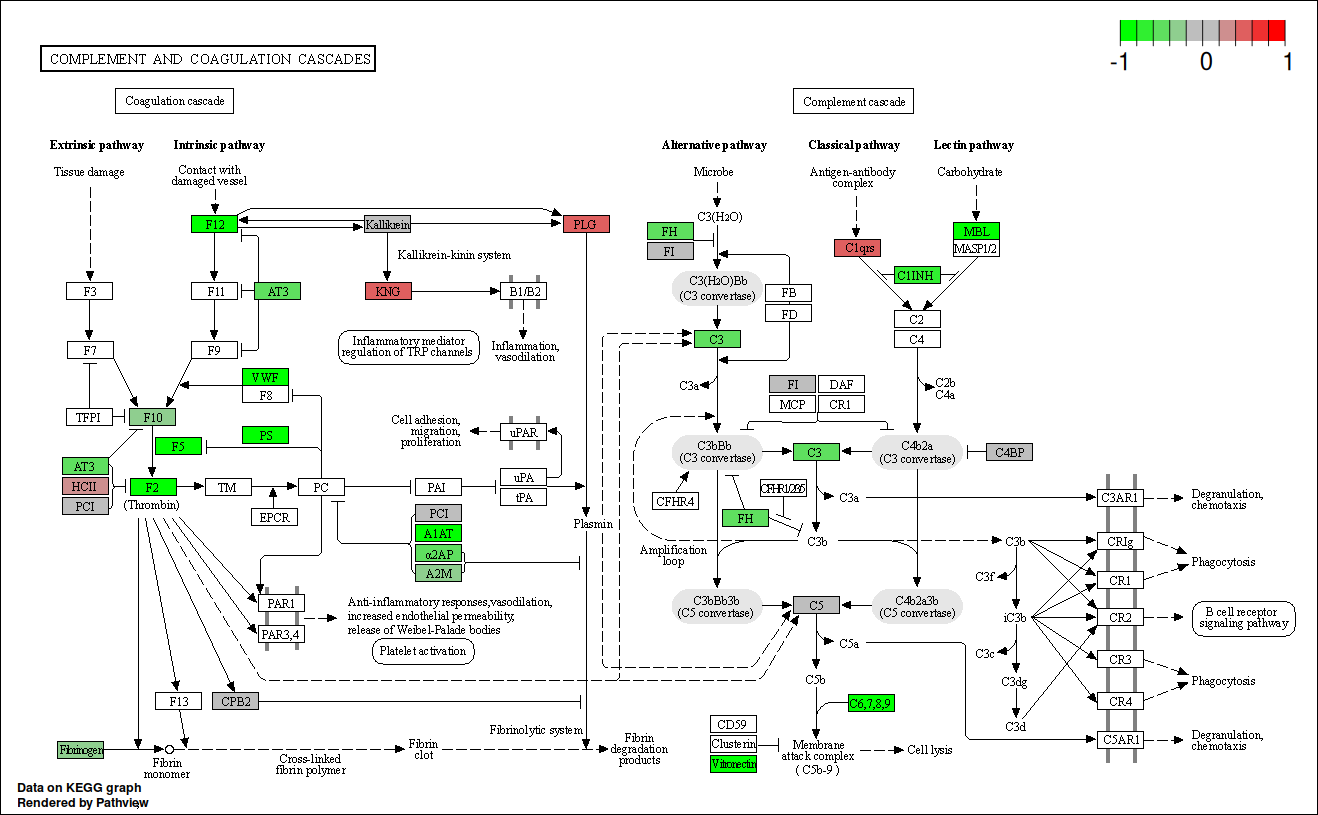
\includegraphics[width=18.31in]{figures/kegg_pathways/hsa04610_pathview} 

}

\caption{KEGG complement cascade pathway annotated with log\(_2\) fold change of proteins in plasma collected 2-weeks post-injury. This compares AIS C SCI patients who experienced an AIS grade improvement and those who did not.}\label{fig:kegg-complement}
\end{figure}

Similarly to the iTRAQ pathway analysis, the label free data analysed via the pathview R package returned the complement and coagulation cascade to be the sole significant KEGG pathway derived from the OpenMS analysed data.
The majority of the proteins present in this pathway were less abundant 2-weeks post-injury in the plasma of AIS C patients who experienced an AIS grade conversion than those who did not (Figure \ref{fig:kegg-complement-chap4}).



\begin{figure}

{\centering 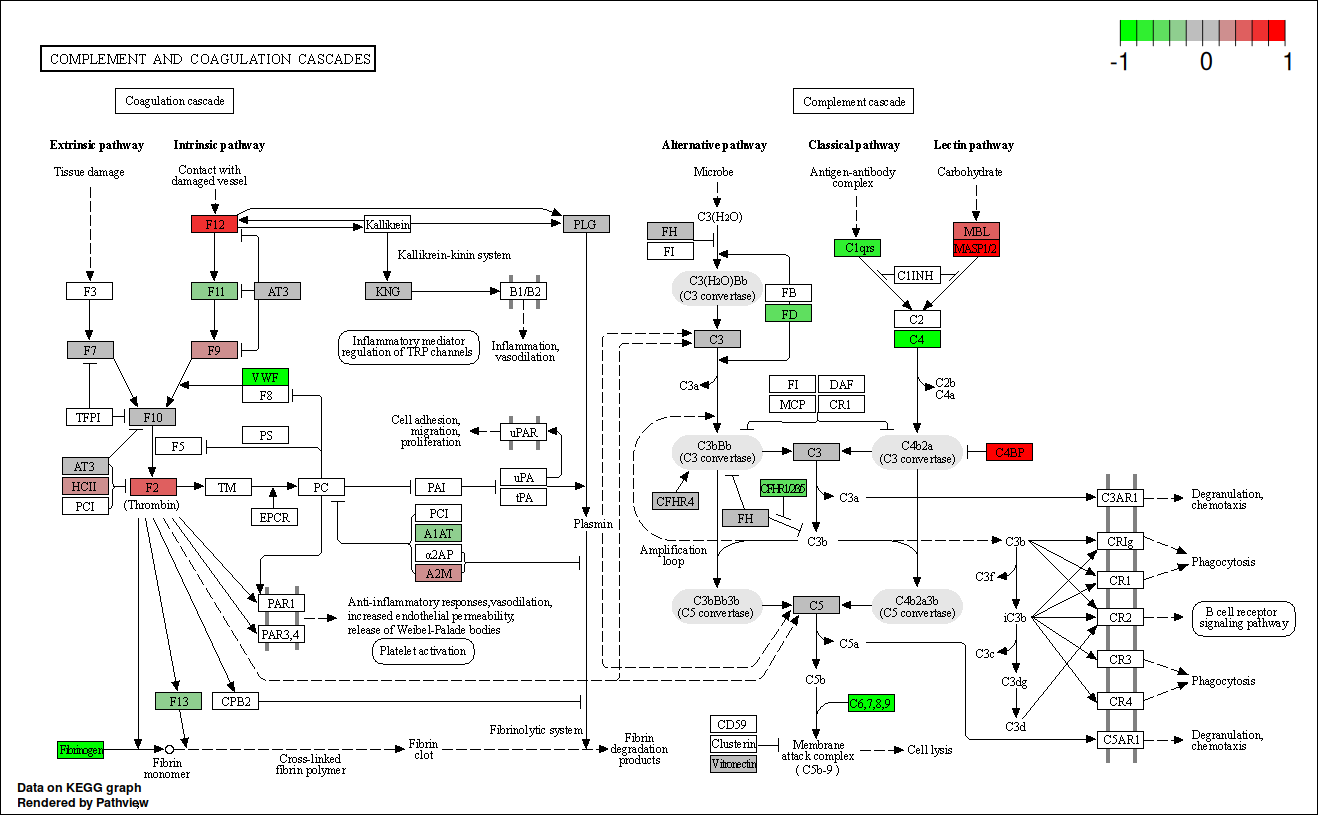
\includegraphics[width=18.31in]{figures/kegg_pathways/hsa04610.pathview_label-free} 

}

\caption{KEGG complement cascade pathway annotated with log\(_2\) fold change of proteins in plasma collected 2-weeks post-injury. This compares AIS C SCI patients who experienced an AIS grade improvement and those who did not.}\label{fig:kegg-complement-chap4}
\end{figure}

\hypertarget{elisas}{%
\subsubsection{ELISAs}\label{elisas}}

No statistically significant difference between groups for A2M abundance in plasma via DuoSet\&reg ELISAs, though there were outliers in the AIS A and D groups, and particularly in the AIS C patients at 3-months who did not experience an AIS grade conversion (Figure \ref{fig:patchwork-2}).
A significant difference was found between AIS C non-improvers at 2-weeks and AIS D for SAA1, with outliers in AIS C non-improvers at 2-weeks, and both AIS C improvers and non-improvers at 3-months post-injury (Figure \ref{fig:patchwork-2}).
For ApoA1 plasma abundance estimated via Quantikine\&reg ELISAs, statistically significant differences were found between AIS C improvers at 2-weeks and both AIS C improvers and non-improvers at 3-months, AIS C 3-month improvers and AIS A and D, and AIS C 3-month non-improvers and AIS A and D (Figure \ref{fig:patchwork-2}).
A statistically significant difference was also found between AIS C improvers and non-improvers at 2-weeks post-injury for RBP4 (Figure \ref{fig:patchwork-2}).



\begin{figure}
\centering
\includegraphics{proteomic_paper_2020-02-11_files/figure-latex/patchwork-2-1.pdf}
\caption{\label{fig:patchwork-2}Normalised estimated concentration of \(\alpha\)-2-macroglobulin (A), serum amyloid A1 (B), apolipoprotein A1 (C) and retinol binding protein 4 (D). Estimates were calculated from the optical density of a standard curve produced via a DuoSet® ELISA. Plasma from each patient that made up the pooled iTRAQ samples was assayed and pairwise t-tests with bonferroni adjusted P-values were performed to assess differential abundance.}
\end{figure}

\hypertarget{stringdb-plots}{%
\subsubsection{STRINGdb plots}\label{stringdb-plots}}

Network interaction plots generated from the OpenMS processed data via \texttt{STRINGdb} revealed that all test groups contained similar proteins, albeit with different abundances, with no distinct group-specific networks observed (Figures \ref{fig:openms-stringdb-acute-c-imp-vs-non}, \ref{fig:openms-stringdb-sub-cs}, \ref{fig:openms-stringdb-acute-sub-c-imp}, \ref{fig:openms-stringdb-acute-sub-c-nonimp}, \ref{fig:openms-stringdb-a-vs-d}, \ref{fig:openms-stringdb-c-vs-d}, \ref{fig:openms-stringdb-c-vs-a}, \ref{fig:openms-stringdb-c-nonimp-vs-a} and \ref{fig:openms-stringdb-c-nonimp-vs-d}).

Network interaction plots generated of the significant proteins via \texttt{STRINGdb} revealed that all groups contained similarly smaller networks, with many proteins with no know interactions in the STRING database (Figures \ref{fig:openms-stringdb-chap4-acute-c-imp-vs-nonimp}, \ref{fig:openms-stringdb-chap4-sub-cs}, \ref{fig:openms-stringdb-chap4-acute-sub-c-imp}, \ref{fig:openms-stringdb-chap4-acute-sub-c-nonimp}, \ref{fig:openms-stringdb-chap4-a-vs-d}, \ref{fig:openms-stringdb-chap4-c-vs-d}, \ref{fig:openms-stringdb-chap4-c-vs-a}, \ref{fig:openms-stringdb-chap4-c-nonimp-vs-a}, \ref{fig:openms-stringdb-chap4-c-nonimp-vs-d}).

\hypertarget{volcano-plots}{%
\subsubsection{Volcano plots}\label{volcano-plots}}

The mean number of down-regulated and up-regulated significant proteins in each group is 10.6, and 6.8.
Between AIS C improvers and non-improvers, 8 and 4 proteins were up- and down-regulated acutely, whereas 6 and 6 were up- and down-regulated subacutely (Figures \ref{fig:volc-plot-c-imp-vs-nonimp} and \ref{fig:volc-plot-subacute-c-imp-vs-nonimp}).
Longitudinally, AIS C acute improvers had 10 up-regulated and 7 down-regulated proteins relative to subacute improvers, while for non-improvers 6 and 12 were up- and down-regulated respectively (Figures \ref{fig:volc-plot-acute-c-imp-vs-subacute-imp} and \ref{fig:volc-plot-acute-c-nonimp-vs-subacute-nonimp}).

\hypertarget{comparing-itraq-and-label-free-proteins}{%
\subsubsection{Comparing iTRAQ and label-free proteins}\label{comparing-itraq-and-label-free-proteins}}

A total of 87 and 79 unique proteinswere identified across the label-free and iTRAQ experiments respectively, with a modest overlap of 26 proteins found using both techniques (Figure \ref{fig:itraq-label-free-venn}).



\begin{figure}

{\centering \includegraphics[width=0.6\linewidth]{proteomic_paper_2020-02-11_files/figure-latex/itraq-label-free-venn-1} 

}

\caption{Venn diagram of the overlap in unique proteins identified from iTRAQ and label-free proteomic experiments analysed via OpenMS.}\label{fig:itraq-label-free-venn}
\end{figure}

\hypertarget{discussion}{%
\section{Discussion}\label{discussion}}

\hypertarget{thesis-itraq-discussion}{%
\subsection{thesis iTRAQ discussion}\label{thesis-itraq-discussion}}

This work builds on the previous chapters (\ref{chap-2-intro}) modelling of routine bloods by analysing the plasma proteome of SCI patients grouped by injury severity and improver status.
In addition to continuing the pursuit of novel biomarkers of SCI, the link between the liver and neurological recovery hinted at in the aforementioned chapter is examined here.

\hypertarget{proteinpilot-and-openms}{%
\subsubsection{ProteinPilot and OpenMS}\label{proteinpilot-and-openms}}

Mass spectrometry is a major technique used in several fields, including metabolomics, lipidomics, interactomics and proteomics, each of which demands a variety of differing approaches to data acquisition and analysis.
Multiple separation methods (liquid chromatography, gas chromatography), fragmentation methods (electron-capture dissociation, electron-transfer dissociation, collision-induced dissociation, etc.) and acquisition strategies (targeted, data-dependent and data-independent) are used in any combination.
With quantification there are different label-free, isotopic or isobaric labelling approaches to employ.
Finally the data analysis may require a database search, as in proteomics and metabolomics, spectral library search or a targeted analysis, depending on the experiment.
This complexity necessitates a multi-interdependent-step workflow tailored to the given experiment.

The manufacturers of mass spectrometers often offer software tailored to their instruments which is often used in the literature.
However, the source code for these software suits is not publicly available, and indeed manufactures often boast of their particular inscrutable proprietary algorithms, often related to peak picking.
This combination of completixy and opacity in analysis methodolotgy can make it extremely difficult to reproducle results from other labs, or even analysis from one's own lab.({``Devil in the Details''} 2011)

To address this issue many open-source (meaning the source code is publicly available) software packages which may perform one or several steps of a complex analysis workflow have been developed.
This issue here is that incorporating multiple software packages together can be both time-consuming and error-prone, and require significant maintenance and documentation to maintain reproducibility.

The OpenMS project aims to address these challenges by providing a flexible software environment, with both pre-assembled workflows that aim to provide best-practices, and allow for more granular control with both command line and Python scripting interfaces.
OpenMS is also integrated with graphical workflow systems such as KNIME and Galaxy, increasing the accessibility of the platform.(Berthold et al. 2009; Goecks et al. 2010)

Here we used both the vendor provided proprietary ProteinPilot and OpenMS to analysis two 4-plex iTRAQ experiments.
We observe that both approaches produce similar results, with a similar number of total proteins identified, a large degree of overlap in the specific proteins identified, and similar fold changes (Figures \ref{fig:openms-pp-venn} and \ref{fig:openms-pp-updown}).
As the results are similar we choose to focus on the OpenMS results due to aforementioned superior reproducibility.

\hypertarget{proteins-identified}{%
\subsubsection{Proteins identified}\label{proteins-identified}}

A total of 79 proteins were identified across both runs for OpenMS, many of which are related in function. (Figure \ref{fig:openms-pp-venn}).
Here we explore the potential these proteins have a biomarkers of SCI.

\hypertarget{alpha-2-macroglobulin}{%
\paragraph{Alpha-2-macroglobulin}\label{alpha-2-macroglobulin}}

A2M is an inhibitor of an unusually diverse array of proteinases by a unique `trapping' mechanism.
The protein achieves this with a peptide stretch, called the ``bait region'', which contains specific cleavage sites for different proteinases.
When a proteinase cleaves the bait region, a conformational change is induced whereby A2M traps the proteinase.
The entrapped enzyme retains active against low molecular weight substrates, whereas activity against high molecular weight substrates is greatly reduced.
Following cleavage in the bait region, a thioester bond is hydrolysed and mediates the covalent binding of the protein to the proteinase.(P. K. Hall et al. 1981; Sottrup-Jensen et al. 1984)
A2M is unique in it's ability to inhibit virtually any protease regardless of it's specificity, origin or catalytic mechanism.(Khan 2004; Lin et al. 2012)

Alpha macroglobulins are an integral part of innate immunity and thus are evolutionarily conserved.(Buresova et al. 2009)
Alpha macroglobulins have significant primary sequence homology with complement components C3, C4 and C5.
The A2M-proteinase complex is cleared from circulation primarily by receptors on hepatocytes.(Bond, Cianciolo, and Pizzo 2007; Travis and Salvesen 1983)
The mammalian receptor for proteinase‐reacted A2M is a low‐density lipoprotein receptor related protein.(Fujiyoshi et al. 2011; Larios and Marzolo 2012; Wyatt and Wilson 2013)

A2Ms definitive function is the delivery of proteinase to an endocytotic proteinase clearance pathway.
A2Ms trap the proteinases released by granulocytes and other cells during inflammation and also regulate the extracellular proteolytic activity resulting from clotting and fibrinolysis.
A2M can also help protect against pathogens as it can trap proteinases from non-human origins as well.
A2M can be recognised and phagocytosed by macrophages and hepatocytes, and it has been proposed to aid in the clearance of defensins and other peptide mediators in inflamed tissues, thus contributing to the regulation and containment of inflammation.(Rehman, Ahsan, and Khan 2013)

Myelin basic protein is released into the circulation following traumatic injury and A2M has been seen to be the only major myelin basic protein-binding protein in human plasma, suggesting A2M protects the immunogenic protein from degradation by proteases and help in its clearance from circulation.(Gunnarsson and Jensen 1998)
A study looking at male infertility after SCI with proteomics found A2M to be elevated approximately 3-fold in the sperm plasma of SCI patients relative to normal controls.(Silva et al. 2016)

We observe A2M to be less abundant in AIS C improvers, within 2-weeks post injury and at 3-months, albeit to a lesser extent (Tables \ref{tab:openms-fc-table} and \ref{tab:proteinpilot-fc-table}).
Similarly, A2M was more abundant is AIS As relative to all groups, and whilst A2M was less abundant in AIS C improvers at 2-weeks compared to AIS Ds, AIS C non-improvers had more A2M than AIS Ds. (Table \ref{tab:openms-fc-table}).
With less A2M there would be more protease activity in these individuals, which may aid in the clearance of damaged tissue, and in particular may lessen the development of an astroglial scar, thus aiding repair.
However, glial scaring is not entirely negative, the primary benefit it offerers is minimising the extent of secondary damage to neighbouring areas by functioning as a barrier around the injury site.
Animal studies have demonstrated that prevention of astroglial scar formation following CNS injury leads to greater lesion size and poorer function outcomes.(Anderson et al. 2016; Wilhelmsson et al. 2006)
Interestingly, a rat study using quantitative liquid chromatography-mass spectrometry with CSF, found A2M to be more abundant in moderately injured animals compared to more severe injuries.(Lubieniecka et al. 2011)

\hypertarget{apolipoproteins}{%
\paragraph{Apolipoproteins}\label{apolipoproteins}}

We found ApoA1, ApoA2, ApoH, ApoL1 and ApoM to be less abundant in AIC improvers at both time points, whereas ApoA4 was more abundant at both time points (Tables \ref{tab:openms-fc-table} and \ref{tab:proteinpilot-fc-table}).
ApoA1 is the main protein component of high-density lipoproteins (HDL).
Plasma HDL include two main apolipoproteins, these being ApoA1 and ApoA2 (\textasciitilde70\% and \textasciitilde20\% of total HDL protein content respectively), but some HDL particles can also contain small amounts of other apolipoproteins, including ApoA4, ApoA5, ApoC, ApoD, ApoE, ApoJ and ApoL.
The primary function of HDL in plasma is the transport of cholesterol, which can have dietary origins, but also be produced endogenously in the liver.

\hypertarget{hdl-activity}{%
\subparagraph{HDL Activity}\label{hdl-activity}}

HDLs have serve a wide range of functions, including contributing to anti-inflammatory activity.
They can limit chemokine secretion from multiple cells types including endothelial cells and monocytes.(Cockerill Gillian W. et al. 1995; Vorst et al. 2013; Bursill Christina A. et al. 2010)
Rats injected with ApoA1 showed significant reduction in expression of CCR2 and CX\(_3\)CR1, the receptors for chemokines of the same name, which play a role in leukocyte migration. (Bursill Christina A. et al. 2010)

HDL is also associated with protection from oxidative damage, also inhibiting the potentially atherogenic oxidised LDL formation.(Anatol, Sandrine, and John 2003)
The exact mechanisms of these antioxidant effect is still actively researched, the enzyme paraoxonase-1, which is present on HDL particles are likely important.(Mackness, Durrington, and Mackness 2004)
Apolipoproteins, including ApoA4 and ApoAE also have antioxidant properties, for example phospholipid hydroperoxidase can be reduced by methionine residues of ApoA1, forming redox-inactive phospholipid hydroxides.(Christison, Rye, and Stocker 1995; Zerrad-Saadi Amal et al. 2009)

HDLs can also suppress proliferation of haematopoietic stem cells, thus reducing leucocytosis and monocytosis.(Yvan-Charvet et al. 2010)
Furthermore, HDLs are implicated in the transport of microRNAs, though the mechanisms of loading the microRNAs and their biological significance is still under study.(Vickers et al. 2011)

ApoE was less abundant in AIS C improvers within 2-weeks and more abundant at 3-months, and more abundant in more severe injury, such as AIS A relative to D or C and in AIS C relative to D (Table \ref{tab:openms-fc-table}).
ApoE is primarily produced by hepatocytes in the liver, but second-most in the brain, synthesised in and secreted by astrocytes, and has been found to an important determinant in response to types of CNS injuries in both animal and human studies.(Teasdale et al. 1997; Poirier 1994)
A key function of ApoE is as a ligand for the LDL receptor family of proteins, which mediate trafficking of cholesterol to neurons, which is vital for axonal growth, and for synapse formation and remodelling.(Xu, Finkelstein, and Adlard 2014)
Additionally, ApoE is implicated in the clearance of neuronal apoptotic bodies.(Elliott et al. 2007)
In humans there are three variants/alleles of ApoE: ApoE2, ApoE3 and ApoE4, which have a frequency of 8.4\%, 77.9\% and 13.7\% globally.(C.-C. Liu et al. 2013)
The variant proteins differ by one or two amino acids and have been found to result in substantial physiological alterations.(Mahley and Rall 2000; Jha et al. 2008)
The presence of the ApoE4 variant has been linked to worse outcomes in SCI and TBI.(Jha et al. 2008; C. Sun et al. 2011; Smith et al. 2006; Friedman et al. 1999)
More specifically, the SCI study reported significantly lower change in the median AIS motor score compared the individuals without the ApoE4 allele during rehabilitation.(Jha et al. 2008)

Prior \emph{in vivo} rodent studies have demonstrated up-regulation of ApoE following SCI and TBI, though ApoE is not observed in neurons of rodents under normal neuropathology, and they only posses a single ApoE allele.(Iwata et al. 2005; Seitz et al. 2003; Mahley, Weisgraber, and Huang 2006)
A separate rodent study reported ApoE levels decreased for the first 3 days post-injury, and then increased peek expression at 7 days post-injury, a similar pattern to our results.(X. Yang et al. 2018)
Furthermore, mouse studies have demonstrated replacement of ApoE in neurons with human ApoE4 have impaired neurite outgrowth compared to replacement with ApoE2 or ApoE3, suggesting ApoE4 interferes with neuroplasticity.(Seitz et al. 2003; White et al. 2001)
The underlying mechanism/s by which ApoE and its alleles effect neuroplasticity is not currently known, but proposals have been made.
One possibility is reduced lipid transport from astrocytes to neurons, potentially impeding the membrane generation required to support axon growth or dendrite sprouting.
ApoE has anti-oxidant properties, so others have suggested impaired anti-oxidant activity may contribute.
ApoE4 has been found to be both secreted less than ApoE2 or ApoE3, and to have inferior anti-oxidant abilities, lending some credence to this idea.(Mishra and Brinton 2018; Miyata and Smith 1996)
Knowing this, whilst ApoE may make for a useful biomarker for SCI, it will be important that particular variants of ApoE a given patient has could be just as important, if not more so, than simple abundance.

\hypertarget{serum-amyloid-a1}{%
\paragraph{Serum Amyloid A1}\label{serum-amyloid-a1}}

SAA1 was less abundant in AIS C improvers at 2-weeks relative to non-improvers, but more abundance in plasma at 3-months (Table \ref{tab:openms-fc-table}.
SAA1 was also more abundant is AIS A relative to less severe injuries, and in AIS Cs relative to Ds (Table \ref{tab:openms-fc-table}.
SAA1 is a major acute-phase protein mainly produced in the liver by hepatocytes in response to infection, tissue injury and malignancy.(L. Sun and Ye 2016)
SAA1 is a precursor of amyloid A (AA), the aberrant deposition of which leads to inflammatory amyloidosis.(Tape et al. 1988)
There are 5 known SAA1 variants, though currently, no indication of substantial functional differences have been identified.(J. Lu et al. 2014)
However, some alleles have been linked to disease, including increased amyloidogenesis and tumour suppression.{[}van der Hilst et al. (2008); lung\_saa1\_2015{]}

During the APR, plasma levels of SAA increase up to 1000-fold, and so serves as a well-established clinical biomarker for inflammatory disorders.(Gabay and Kushner 1999)
SAA isoforms produced by hepatocytes during an APR are swiftly released into the blood where they associate with HDL, displacing ApoA1 and becoming an apolipoprotein of HDL.(Banka et al. 1995; Benditt and Eriksen 1977)
Reverse cholesterol transport, whereby cholesterol in non-hepatic tissues is transported back to the liver, is conducted via plasma components such as HDL, ABCA1 and ABCG1.
ApoA1 acts as an acceptor for cholesterol in this process, and studies have found that SAA in lipid-free form can similarly function as a cholesterol acceptor for ABCA1.
Whilst SAA is though to be an important facet of lipid metabolism, its role is likely complex as mice knockout studies which eliminate SAA1 and SAA1 have shown little effect on cholesterol transport, HDL levels and ApoA1 clearance.(de Beer et al. 2010, 2011)
These studies indicate that the \emph{in vivo} functions of SAA related to lipid metabolism are more complex than prior \emph{in vitro} studies implied.

SAA1 can both induce anti-inflammatory interleukin 10 (IL-10)-secreting neutrophils, but also promotes the interaction of invariant natural killer T cells with those neutrophils, which limits their suppressive activity by diminishing the production of IL-10 and enhancing the production of IL-12, indicating that SAA1 can have both pro- and anti-inflammatory effects.(Santo et al. 2010)
There has however been conflicting results reported of SAAs cytokine induction abilities, and some studies have suggested that recombinant human SAA1 provided by some vendors may have additional cytokine-inducing actiity due the altered amino acid sequence.(M.-H. Kim et al. 2013)

Macrophages are a major source of SAA in inflammatory tissues, and elevated SAA production has been observed in rheumatoid arthritis, Crohn's disease, Type 2 diabetes and atherosclerosis.(Marzi et al. 2013; Dong et al. 2011; Vallon et al. 2001; C, F, and B 1997; Meek, Urieli-Shoval, and Benditt 1994)
SAA binding to HDL was reported to increase affinity for macrophages whilst decreasing affinity for hepatocytes.(R. Kisilevsky and Subrahmanyan 1992)
This change is thought to favour the removal of cholesterol from site of inflammation.(R. Kisilevsky 1991)
SAA inhibits the binding of the scavenger receptor SR-BI and cholesterol efflux is enhanced in a SR-BI-dependent manner.(Cai et al. 2005; van der Westhuyzen et al. 2005)
It has been suggested that the SR-BI-mediated re-uptake of cholesterol underpins the role of SAA in cholesterol recycling during tissue repair, where a great deal of cholesterol is required.(Robert Kisilevsky and Manley 2012)

In blood circulation SAA1 may also function as a immune opsonin for increased neutrophil uptake of Gram-negative bacteria.(Shah, Hari-Dass, and Raynes 2006)
Both human and mouse SAA proteins have been found to bind retinol with nanomolar affinity that limits bacterial burden in tissues after acute infection.(Derebe et al. 2014)
Retinol is important to the body's response to microbial infection, so SAA may also have a role in limiting bacterial burden, particularly in the liver, spleen and intestine.
The aforementioned study demonstrated that mice lacking in both SAA1 and SAA2 have a higher bacterial burden in the liver and spleen following infection.(Derebe et al. 2014)
All 3 SAA isoforms are found in intestinal epithelium, which is exposed to the gut microbiome, in mice.
The anti-bacterial properties of SAA isoforms may therefore explain the role of SAA as an acute-phase protein that protects the host in tissues and organs exposed to bacteria.

\hypertarget{retinol-binding-protein-4-rbp4}{%
\paragraph{Retinol-binding protein 4 (RBP4)}\label{retinol-binding-protein-4-rbp4}}

In plasma within 2-weeks post-injury, RBP4 was less abundant in AIS C improvers relative to AIS D and A, and more abundant in AIS C non-improvers again, relative to AIS D and A (Table \ref{tab:openms-fc-table}.
Similarly, AIS A plasma had more RBP4 compared to AIS D, and AIS C improvers were also more abundant in RBP4 compared to non-improvers at both 2-weeks and 3-months post-injury (Table \ref{tab:openms-fc-table}.

Vitamin A is a collective term for a group of fat-soluble compounds with a range of essential biological activities including aspects of growth, vision and metabolism.(Blomhoff and Blomhoff 2006)
Following dietary absorption, vitamin A is ferried from the intestine, with chylomicrons as retinyl esters, to tissues for immediate use or the liver for storage in hepatic stellate cells.
A subsequent dietary deficiency of vitamin A will result in these liver stores being mobilised by hydrolysing the retinyl esters to release retinol.
The retinol is then bound by RBP4, which is also mainly synthesised in the liver, and secreted into circulation from hepatocytes, whereupon it is bound by an additional transport protein, transthyretin.(P. A. Peterson 1971)
The membrane plasma protein STRA6 facilitates retinol transport from RBPs across the cell membrane.(Berry et al. 2012)
Once delivered to target cells, retinol can either be converted to retinaldehyde, which is required for functional vision, or oxidised to retinoic acid, which is a ligand for nuclear receptors, thus regulating gene expression.(Lane and Bailey 2005; J. E. Balmer and Blomhoff 2002)

RBPs are localised in the ventral region, associated with motor neurons, in the mammalian developing neural tube.(Pierani et al. 1999; Maden, Ong, and Chytil 1990)
The role of retinoid signalling in spinal cord and motor neuron differentiation, including development of regions of the spinal cord has been outlined, and implies a possible involvement in maintaining motor neuron integrity.(Colbert et al. 1995; Sockanathan and Jessell 1998)

The mRNA of a rodent homologue of RBP, named cytosolic retinol binding protein, was found to be up-regulated at 24 hours post-SCI and may promote cell proliferation and regeneration by increasing retinoid metabolism.(Song et al. 2001; Hurst et al. 1999)
Another study of amyotrophic lateral sclerosis (ALS), a neurodegenerative disease, comparing gene expression between post-mortem spinal cord samples of ALS and controls also observed up-regulation of RBP1 in ALS spinal cord.(Malaspina, Kaushik, and Belleroche 2001)
Furthermore, a transgenic mouse study reported retinoid signalling may contribute to the retained plasticity and regenerative potential of the mature spinal cord.(Haskell et al. 2002)

The results found here support these findings for AIS C improvers relative to non-improvers as improver had increased levels of RBP4.
Whether this is due to increased expression or due to higher vitamin A intake is unclear from this data, though at 3-months post-injury this is still that case even though patients diets could be more similar throughout hospital admission.

\hypertarget{metabolism-and-sci}{%
\subsubsection{Metabolism and SCI}\label{metabolism-and-sci}}

\hypertarget{acute-phase-response}{%
\paragraph{Acute phase response}\label{acute-phase-response}}

The bodies first response to injury or infections, including SCI, is often referred to as the ``acute phase response'' (APR), which is non-specific, innate reaction that precedes more specific and situational immune reactions.(Gordon and Koj 1985; Gruys et al. 2005)
This systemic response is largely coordinated by factors released from the liver, but the APRs effects extend to multiple peripheral organs including the kidneys, lungs and spleen.(Bao et al. 2012; S. J. Campbell, Zahid, et al. 2008; Fleming et al. 2012; Gris, Hamilton, and Weaver 2008)
This hepatic response is typically transient and quickly fades, but prolonged liver inflammation and pathology has been observed in rodent SCI models.(Goodus et al. 2018; Sauerbeck et al. 2014)

Basic liver functions are chronically impaired by SCI, including metabolising carbohydrates, fats and proteins, storage of minerals vitamins and glycogen and filtering blood from the digestive tract.(García-López et al. 2007; DeLeve 2007; Farkas and Gater 2018; Chow et al. 2012; Sauerbeck et al. 2014)
This is likely related to the elevated incidence of metabolic disease in the SCI cohort, including insulin resistance, impaired glucose tolerance and cardiovascular disease.(Bauman and Spungen 2001; Maruyama et al. 2008; Lee et al. 2004; J. Myers, Lee, and Kiratli 2007)
Long-term survival is noticeably lower relative to the general population and, whilst mortality in the first 2 year following SCI has decreased in recent decades, long-term survival has not.(Strauss et al. 2006; Shavelle et al. 2015)
More recently, a longitudinal study found SCI patients had a significantly higher incidence of acute pancreatitis relative to a matched healthy cohort.(Ho, Yeh, and Pan 2021)

The acute (1-7 days) liver response to SCI is well documented; the inflammatory cytokines including TNF\(\alpha\), IL-1\(\alpha\), IL-1\(\beta\) and IL-6, released at the injury site, reach the liver through the bloodstream.(Fleming et al. 2012; Hundt et al. 2011)
This provokes the liver to enter the APR and produce acute phase proteins (APPs) thus stimulating a greater immune response.(Anthony and Couch 2014; Fleming et al. 2012)
The hepatocytes that make up the majority of the liver biomass, express receptors that bind the aforementioned inflammatory cytokines; similarly the hepatic macrophage Kupffer cells also bind these cytokines, complement proteins and lipopolysaccharide (LPS) and swiftly remove microorganisms, endotoxins and other debris from the blood.(C.-Y. Yang et al. 2013; Szalai et al. 2000; Crispe 2016; S. J. Campbell et al. 2005)
Hepatic stellate cells act as sensors of tissue integrity by exposure to signals of oxidative stress, danger/pathogen associated molecular patterns (DAMPs/PAMPs), chemokines/cytokines and factors secreted from neighbour hepatic cells, and can stimulate innate immunity by releasing cytokines and as antigen presenting cells during the APR. (Weiskirchen and Tacke 2014; Fujita and Narumiya 2016)

SCI studies in rodent and canine models have found the APPs serum amyloid (SA) A, SAP, CRP, fibrinogen, haptoglobin and a1-antichymotrypsin are elevated 4-24 hours post-injury in blood.(Pepys and Baltz 1983; Gabay and Kushner 1999; J. C. E. Hall et al. 2012; Steel and Whitehead 1994)
In rodents, hepatic CD68 mRNA is observed to be elevated within 24 hours post-SCI and CD68+ Kupffer cell numbers increase during the first 7 days post-SCI.(Sauerbeck et al. 2014)

Furthermore, it has been suggested that liver inflammation and Kupffer cells activity promote recruitment of leukocytes to the injury site in brain or spinal trauma, potentially enhancing CNS injury.(Anthony and Couch 2014; S. J. Campbell et al. 2005)
For example, a rodent study demonstrated depletion of Kupffer cells prior to injury resulted in few neutrophils infiltrating the injury site.(S. J. Campbell, Zahid, et al. 2008; S. J. Campbell, Anthony, et al. 2008)

\hypertarget{microbiome-sci}{%
\subsubsection{Microbiome \& SCI}\label{microbiome-sci}}

Circulating factors from the injury site are not the only potential driver of hepatic inflammation.
Within 24 hours post-SCI in rodents tight junctions between epithelial cells become more permeable, thus allowing gut bacteria and the endotoxins they can produce to enter the bloodstream.(J. Liu et al. 2004)
This will reach the liver through the portal vein where Kupffer cells function as a ``first line of defence''.(Jenne and Kubes 2013; M. L. Balmer et al. 2014)
It has been proposed that elevated LPS+ endotoxins caused by the post-SCI ``leaky gut'' causes acute liver inflammation by overloading hepatic filtrations capacity, allowing microbes to bypass the liver and elicit systemic inflammation.(J. Liu et al. 2004; O'Connor et al. 2018)
The binding of LPS to Kupffer cells results in the production of a range of growth factors, including TNF-\(\alpha\), multiple interleukins and reactive oxygen species (ROS), stimulating bone-marrow-derived monocytes and neutrophils to infiltrate the liver.(S. A. Myers et al. 2019; Milosevic et al. 2019; Kazankov et al. 2019)
A rodent study found transcription factors for tight junctions down-regulated following SCI, and that application of probiotics improved neurological outcomes.(Kigerl, Mostacada, and Popovich 2018; Kigerl et al. 2016)
Human studies of the microbiome post-SCI have also demonstrated dysbiosis, both chronically and more acutely post-injury.(Zhang et al. 2018; Gungor et al. 2016; Bazzocchi et al. 2021)

\hypertarget{drivers-of-liver-steatosis}{%
\subsubsection{Drivers of liver steatosis}\label{drivers-of-liver-steatosis}}

Steatosis, the abnormal retention of lipids within cells or organs, most commonly associated with the liver, has been observed to increase in rodents during the first week post-injury.(Sauerbeck et al. 2014)
The liver takes up circulating fatty acids, and when levels exceed the oxidative and secretory limits of the liver, hepatocytes store the excess as triglycerides.(Diraison and Beylot 1998)
Adipose tissue lipolysis during elevated sympathetic activity leading to spikes in circulating fatty acids has been reported in human subjects following SCI.(Karlsson 1999)

\emph{De novo} lipogenesis occurring within the liver can also drive hepatic steatosis.(Lavoie and Gauthier 2006)
Ceramides are lipid signalling molecules and regulators of apoptosis and inflammation; they can contribute to insulin resistance, oxidative stress and inflammation-induce liver adiposity through sustained Toll-like-receptor(TRL)-4 activation.(Schilling et al. 2013; Bhargava and Lee 2012; Pagadala et al. 2012)
If released into the circulatory system, ceramides can cause CNS toxicity, including oxidative damage and changes to the aggregation of proteins associated with diseases such as Parkinson's, Huntington's and Alzheimer's.(Pagadala et al. 2012; Vidaurre et al. 2014; Czubowicz et al. 2019)
Mature and precursors of hepatic ceramides and enzymes which contribute to ceramide synthesis are elevated by 1 day post-injury.(Sauerbeck et al. 2014)
Endotoxins can also stimulated the synthesis of ceramides and so the aforementioned ``leaky gut'' may also contribute to this elevation.(Chang et al. 2011)
Ceramide synthesis and lipogenesis genes are also stimulated by TNF-\(\alpha\), which, as touched on in the general introduction (\ref{chap-1-biomarkers}), has been found to be elevated post-SCI, and associated with differential neurological recovery.(Davies, Hayes, and Dekaban 2007; Hasturk et al. 2009; Biglari et al. 2015; Sauerbeck et al. 2014; Bikman 2012)

\hypertarget{chronic-liver-inflammation-in-sci}{%
\subsubsection{Chronic liver inflammation in SCI}\label{chronic-liver-inflammation-in-sci}}

The hepatic APR and associated inflammation that typically follows bodily trauma, subsequently rapidly subsides, whereas post-SCI this hepatic inflammation persists chronically.
This chronic phase may be due in part to long-term changes in intestinal permeability via fewer tight junctions in intestinal epithelial cells, resulting in gut dysbiosis.(Milosevic et al. 2019; O'Connor et al. 2018; Kigerl, Mostacada, and Popovich 2018; Kigerl et al. 2016)
Bacterial translocation and gut dysbiosis can be the result of non-mechanical intestinal obstruction, impaired intestinal motility and systemic immune suppression, all of which are potential complications of SCI.(Balzan et al. 2007)
Specifically, butyrate-producing bacteria have been found to be reduced in SCI relative to a healthy cohort.(Gungor et al. 2016)
Butyrate is known to modulate epithelial differentiation and cell growth, and suppress macrophages, including CNS inflammation, thus the reduction in butyrate from bacteria may contribute to recovery post-SCI, though links to the liver specifically have not yet been studied.(H. J. Kim et al. 2007; Arpaia et al. 2013; Park et al. 2005; P. S. Chen et al. 2007)

LPS is another potential modulator of post-SCI chronic liver physiology.
Kupffer cells, hepatic endothelial cells and hepatocytes all participate in the clearance of LPS via CD14- and TLR4-dependent mechanisms.(Mimura et al. 1995; van Oosten et al. 2001; Vodovotz et al. 2001)
LPS induced the release of factors such as TNF-\(\alpha\)

\hypertarget{longitudinal-metabolic-health}{%
\subsubsection{Longitudinal metabolic health}\label{longitudinal-metabolic-health}}

Prior work has found at least 25\% of acute SCI patients to be obese, which is well known to induce low-level systemic inflammation, and that this cohort has significantly worse outcomes compared to non-obese SCI patients (Stenson et al. 2011).
Alcohol abuse has also been associated with poorer SCI neurological outcomes (Elliot et al. 2002).
Furthermore, advancing age is associated with increased liver inflammation and the SCI population has followed the general populations ageing trend (Bertolotti et al. 2014; Y. Chen, He, and DeVivo 2016).
Taken together, it is not unreasonable to assume that a large number of SCI patients may have pre-existing liver inflammation at injury.
This may be an important differentiator that contributes to the degree of neurological recovery a given patient may experience.
Future experiments investigating neurological outcomes of SCI may benefit from establishing parameters of metabolic health, including the composition of the microbiome, as close to injury as possible, and potentially monitoring changes in these parameters longitudinally.

\hypertarget{validation-of-results}{%
\subsubsection{Validation of results}\label{validation-of-results}}

The ELISAs used to validate the proteomic data often did not demonstrate significant differences between the groups (Figures \ref{fig:elisa-sig-plots1}, \ref{fig:elisa-sig-plots2}, \ref{fig:elisa-sig-plots3} and \ref{fig:elisa-sig-plots4}).
This may be in part to the individual variability of the samples.
However, the trends of the data do largely reflect those found in the iTRAQ data, suggesting that with greater statistical power there may be a more robust validation.
Furthermore, the ApoA1 ELISAs resulted in the most significant differences, and was the only Quantikine\&reg kit used (Figure \ref{fig:elisa-sig-plots3}).
As the Quantikine\&reg kits are highly optimised, including for use with plasma, whereas the DuoSet\&regs, which were used for the other proteins, are not.
Future studies should therefore consider either simply using Quantikine\&reg kits, or ensure good optimisation of the DuoSet\&reg kits in advance.
These results are also corroborated by a recent label-free proteomic SCI study, using a rodent model, which reported similar proteins associated with complement cascade, including A2M and C3.(Yao et al. 2021)

\hypertarget{chap-3-conc}{%
\subsubsection{Conclusion}\label{chap-3-conc}}

This work shows that proteins associated with the complement cascade, and apolipoproteins in particular, have potential as prognostic biomarkers for SCI.
For some of these biomarkers, ApoE in particular, it may not be pure abundance, but also the particular allele of the patient that may provide valuable insight.
However, the relatively small number of proteins identified here is a limitation, likely due to highly abundant proteins impacting the dynamic range of the samples.
The pooling of samples also obscures individual variability in protein abundance.
Subsequent proteomics experiments using label-free techniques, and depletion of highly abundant proteins may allow for more in-depth pathway analysis.
These results, in concert with the prior chapters findings (\ref{chap-2-conclusion}), provide further evidence of a link between metabolic function and functional neurological recovery post-SCI.
Further work is needed elucidate the precise biochemistry at play, and perhaps more importantly, whether modulation of these pathways has the potential to improve outcomes.
Experiments that closely monitor the liver, modify diet and analyse metabolites, particularly longitudinally post-injury, would all give further insight into this relationship.

\hypertarget{thesis-label-free-discussion}{%
\subsection{thesis label-free discussion}\label{thesis-label-free-discussion}}

As outlined previously (\ref{chap-3-conc}), two key limitations of the iTRAQ experiments were the pooling of samples, which prevents statistically robust group-wise comparisons, and the high dynamic range of protein abundances in plasma potentially obscuring less abundant proteins.
This work seeks to address these factors by a combination of Proteominer™ beads to shrink the dynamic range of protein abundances, and by not pooling samples.

\hypertarget{proteins-identified-1}{%
\subsubsection{Proteins identified}\label{proteins-identified-1}}

A total of 87 proteins were identified, many of which were only detected in one group.
Proteins only present in limited groups could be highly suited for use as biomarkers as binary indictors are much simpler to test for, and suggest more dramatic biological differences.
Here we explore the potential these proteins have a biomarkers of SCI.

\hypertarget{peroxiredoxins}{%
\subparagraph{Peroxiredoxins}\label{peroxiredoxins}}

Peroxiredoxins are a large and highly conserved family of enzymes that reduce peroxides.
Peroxiredoxin 2 (PRX-2) is highly abundant in RBCs and intracellularly serves as an important anti-oxidant role in various cells types, including neurons.(Low, Hampton, and Winterbourn 2008)
By contrast, extracellular PRX-2 has been suggested to act as an inflammatory DAMP, leading microglia and macrophages to release a plethora of pro-inflammatory factors.(Salzano et al. 2014; Garcia-Bonilla and Iadecola 2012; Shichita et al. 2012)
An \emph{in vitro} primary neurons and microglia co-culture study reported PRX-2 activating microglia via TLR-4, potentially leading to neuronal apoptosis.(Y. Lu et al. 2018)
A mouse study found over-expression of PRX-2 attenuated oxidative stress and neuronal apoptosis following subarachnoid haemorrhage.(Y. Lu et al. 2019)
Over-expression of PRX-2 is speculated to protect again ischaemic neuronal injury by modulating the redox-sensitive thioredoxin-apoptosis signal-regulating kinase (ASK) 1 signalling complex.(Gan et al. 2012)
Several molecular chaperones can interact with ASK1, including thioredoxin and TNF receptor-associated factor 6.(Matsuzawa et al. 2005)
The dissociation of the thioredoxin-ASK1 complex activates ASK1.
PRX-2 is oxidised after scavenging free radicals, whereupon its antioxidantive activity is reduced.
This inactivation can be reversed by the thioredoxin-thioredoxin reductase system, whereby oxidised PRX-2 can regain its activity by reducing thioredoxin, leading to the dissociation of the thioredoxin-ASK1 complex.(Rhee and Woo 2011)
Additionally, oxidised PRX-1 can inhibit ASK1-induced apoptosis via the thioredoxin-binding domain on ASK1.(S. Y. Kim, Kim, and Lee 2008)

PRX-2 was found to be present in AIS C improvers and AIS D patients acutely, and in AIS A and D patients subacutely.
The differences in abundance between these groups was not statistically significant, though acute AIS D had less PRX-2 relative to subacute AIS D (log\(_2\) fold change -1.9) and subacute AIS A also had less abundant PRX-2 relative to subacute AIS D (log\(_2\) fold change -1.7).
The presence of PRX-2 in acute AIS C improvers and absence in acute C non-improvers suggests the protein could indicate a more protective action against oxidative stress, and implies the protein has potential value as a biomarker of functional outcomes.
Similarly, PRX-2 may be acting as a healthy response to trauma-induced oxidative stress in both acute AIS D, although the persistence to the subacute time-point is less clear.
Likewise, the presence of PRX-2 in AIS A subacutely, but not acutely is more perplexing.
It should be noted that as plasma was used and cells lysed, so there is no distinguishing between intracellular and extracellular PRX-2.
Perhaps in the more severe AIS A injury, secondary injuries, including oxidative stress, are greater and so persist to the subacute time-point.
The acute absence may be a result of an overwhelmed physiology unable to respond or prioritise managing oxidative stress.

\hypertarget{neuroinflammation-post-sci}{%
\paragraph{Neuroinflammation post-SCI}\label{neuroinflammation-post-sci}}

The neuro-inflammatory response begins immediately post-trauma, and involves a complex series of events that can persist well into the chronic phase.
The sudden emergence of necrotic cell debris and associated DAMPs lead surviving CNS-resident cells to produce cytokines, complement factors and ROS.
Within minutes CNS cells at the lesion site have been found to secrete several pro-inflammatory mediators, including TNF-\(\alpha\) and interleukins, in both rodent models and human patients with SCI.(Pineau and Lacroix 2006; Chandrasekar et al. 2017; Dalgard et al. 2012; Bastien et al. 2015)
The resulting inflammatory response occurs in parallel to the mechanical destruction of the blood-spinal cord barrier, and the development of tissue oedema and ischaemia combine to propagate damage to parts of the cord spared by the initial trauma.(Maikos and Shreiber 2007; Ahuja et al. 2017)

The microglial population at the lesion site have been observed to be significantly depleted immediately post-injury, due to death via both the apoptosis and mechanical injury in a rodent model.(Bellver-Landete et al. 2019)
Surviving microglia change in shape and migration patterns, and begin to produce ROS, oxidative metabolites an pro-inflammatory cytokines.(Pineau and Lacroix 2006; Bastien and Lacroix 2014)
These cells can associate with damaged axons rapidly post-injury, but are thought to not actively phagocytose these cells until approximately 4 days post-trauma.(Bellver-Landete et al. 2019; Pineau and Lacroix 2006; Greenhalgh and David 2014)

The following hours and days post-injury are characterised by a substantive complement system activation and sequential leukocyte migration from the periphery into the injured neural parenchyma.(Brennan et al. 2015; S. L. Peterson and Anderson 2014; Qiao et al. 2006)
Curiously, though the breakdown of the BSCB would presumably allow unrestricted access of circulating leukocytes into the injured cord segment, recruitment of these cells remains a highly controlled process.(Beck et al. 2010; Brennan et al. 2019)
A mouse study reported lymphocytes, which account for approximately 80\% of circulating leukocytes, only enter the cord in substantial numbers at least several weeks to months post-injury.(Beck et al. 2010)
Early infiltrate is instead largely comprised of myeloid cells, predominantly neutrophils, which are a minority of circulating cells but are the swiftest peripheral responders to SCI, with studies detecting them at the lesion site within 4 hours of injury.(Wright et al. 2010)
Neutrophil numbers have been reported to peak at 1 day post-trauma, but also to remain at the site for a minimum of 42 days post-injury.(Okada 2016; Kigerl, McGaughy, and Popovich 2006)

This neutrophil recruitment is often viewed as principally detrimental to recovery following SCI, but also wound healing more generally.
A recent study found circulating neutrophil numbers in admission bloods from human SCI patients were negatively correlated with patient outcomes at discharge.(Brennan et al. 2019)
The same study utilising a contusive SCI mouse model, showed the extent of neutrophil presence at the lesion site inversely correlated with neurological outcomes, and depletion of said cells with an antibody against Ly6G improver recovery of motor function.(Brennan et al. 2019)
However, other studies have suggested neutrophil activity which potentially benefits SCI recovery.
A transgenic mouse contusion model study showed over-expression of secretory leukocyte protease inhibitor, which can arise from neutrophils and activated macrophages, improved locomotive functional outcomes, and reduced markers of secondary injury.(Ghasemlou et al. 2010)
Another study, using a peripheral nerve injury mouse model, reported neutrophil infiltration and associated cytokine/chemokine production was vital for clearance of myelin debris.(Lindborg, Mack, and Zigmond 2017)
Additionally, another study using a mouse contusion model found increased lesion sizes and impaired neurological outcomes following neutrophil depletion, though the Gr-1 antibody used also depletes inflammatory monocytes, muddying the picture somewhat.(Stirling et al. 2009)
Regardless, it is clear that the complexity of the role neutrophils play in the SCI response extends beyond any simple binary beneficial/harmful distinction.

Moving forward in the SCI pathology, newly proliferated and recruited microglia begin actively phagocytosing necrotic cell debris, and begin accumulating around the lesion epicentre.(Greenhalgh and David 2014; Bellver-Landete et al. 2019; Pineau and Lacroix 2006)
The presence of microglia appears to be vital, particularly during the first week post-SCI, as depletion via the colony stimulating factor-1 inhibitor PLX5622 has been linked to substantially worsened functional outcomes.(Bellver-Landete et al. 2019; Brennan et al. 2018)
Relatedly, another mouse SCI model study found early enhancement of microglial activation can reduce secondary pathology.(Stirling et al. 2014)

Circulating inflammatory monocytes are also recruited during the first days post-trauma.
Adoptive transfer experiments have shown recruitment to pick up at approximately 3 days post-injury, and peak at 7 days.(Blomster et al. 2013)
Whilst monocyte turnover at the lesion appears to be high, infiltrating monocyte-derived macrophages remain at the site of weeks to months post-trauma.(Blomster et al. 2013; Shechter et al. 2009)
Interestingly, the timing of monocyte recruitment appears to be delayed relative to non-neurological tissue injury.
For instance, monocytes are reported to be rapidly recruited to the heart following a myocardial infarction, as early as 1 day post-injury, and their numbers return to baseline by roughly 16 days post-injury.(Nahrendorf et al. 2007)

Owing to the diversity of monocyte subsets and macrophage phenotypes, a complete understanding of their role with respect to SCI pathology is still lacking, and requires under active research.(David and Kroner 2011)
Some polarisation states associated with recruited macrophages are thought to be implicated in propagating secondary injury via fibrotic scar formation and demyelination of axons.(Kigerl et al. 2009; Popovich et al. 1999; Zhu et al. 2015)
Similarly, several studies have reported a reduction in infiltration of monocytes/macrophages is associated with better SCI outcomes.(Kigerl et al. 2009; Zhu et al. 2015; Horn et al. 2008)
Conversely, others have found depletion o circulating monocytes/macrophages significantly increased lesion size and results in worse function outcome, with restoration of blood monocyte numbers attenuating this phenotype.(Shechter et al. 2009)
More recent \emph{in vitro} studies suggested blood-derived macrophages can suppress microglial phagocytosis without reducing microglial proliferation and extension of processes.(Greenhalgh and David 2014; Greenhalgh et al. 2018)
This literature represents and ongoing controversy over the role of monocytes/macrophages in relation to recovery post-SCI.
Importantly, many of these studies are based on somewhat crude depletion of cell types, with little discrimination paid toward any potential subpopulations and/or cell polarisation status.
Given the shear complexity of the pathology at play, more nuanced approaches will likely be needed in future studies to paint a more complete picture.

B cell recruitment is yet wave of immune cell infiltration, thought to occur several days post-injury.
These cells can form follicle-like structures in combination with T cells, microglia and macrophages from roughly 28 days post-trauma, and remain present and the lesion well into the chronic phase of SCI.(Ankeny, Guan, and Popovich 2009)
Whilst the extent of B cell presence has been reported to vary between animals, they have been correlated with self-reactive antibodies that recognise epitopes within protein homogenates of the spinal cord.(G. Sun et al. 2017)
Adoptive transfer experiments in a mouse model isolated antibodies from SCI mice, and found injected them into the neural parenchyma of naïve animals induced significant damage, whereas mice lacking B cells have improved recovery post-SCI.(Ankeny, Guan, and Popovich 2009)

Move evidence is needed to establish whether these self-reactive antibodies precede an autoimmune event, or signify a autoimmune disease.
Alternatively, they may serve as a mechanism for opsonisation and debris clearance from the lesion site.(Nagele et al. 2013)
Naturally occurring autoantibodies with well-established role in tissue regeneration and repair have been found to be elevated following SCI.(Palmers et al. 2016; Arevalo-Martin et al. 2018)
Much like the aforementioned monocyte/macrophage controversy, it should be pointed out that any positive effects of these autoantibodies does not preclude any simultaneous negative impacts which could be modulated.
For instance, another study reported naturally occurring IgM antibodies contribute to secondary injury during the more acute phase post-SCI.(Narang et al. 2017)

Neuro-inflammation is less understood at the chronic phase of SCI, as most studies focus on the first hours and days post-injury.
By this stage, the glial scar has established a well-defined border between the lesion core and the health tissue flanking it.(Sofroniew and Vinters 2010)
Infiltrating immune cells are largely restricted to within the lesion itself, as opposed to the surrounding spared tissue.
B and T cells, macrophages and neutrophils have all been detected here many months post-trauma.(Beck et al. 2010; Ankeny, Guan, and Popovich 2009; Prüss et al. 2011)
The chronic phase is also marked by substantial metabolic dysfunction, characterised by reduced lipid metabolites and increased oxidative stress, in addition to elevated pro-inflammatory mediators.(Dulin et al. 2013)

There are fewer studies that attempt to elucidate the underlying mechanisms driving this non-resolving inflammatory response in the chronic phase of SCI.
One study suggested communication with infiltrating monocytes suppresses chronic microglial activation and inflammation after SCI.(Greenhalgh et al. 2018)
Interruption of this communication was linked to worsened function outcomes, implying the initial microglial response to trauma may be beneficial, their protracted activation can eventually become detrimental.(Bellver-Landete et al. 2019; Greenhalgh et al. 2018)
Furthermore, a rodent model study of chronic SCI, found use of the anti-inflammatory drug licofelone, applied daily for 1 month at 8 months post-injury, observed some improvement to metabolic functions, but no benefit to locomotor function.(Dulin et al. 2013)
To summarise, understanding of persistent inflammation during the chronic phase of SCI is lacking, and particularly complicated by the plateaus in locomotive recovery that typically occurs well before the chronic SCI phase is reached.
Thus, there is a need for further studies to uncover the role of the various immune cell populations with respect to ongoing neurological dysfunction and pathology during the chronic phase of SCI.

\hypertarget{intravenous-immunoglobulin}{%
\subparagraph{Intravenous immunoglobulin}\label{intravenous-immunoglobulin}}

Intravenous immunoglobulin (IVIG) is increasingly used as an immunomodulatory strategy for managing acute neurological conditions, including neurotrauma.
Originally developed as an antibody replacement therapy for immunodeficiency disorders, IVIG is a product comprised primarily of immunoglobulin G (IgG) taken from the blood plasma of healthy donors.(Bayry, Negi, and Kaveri 2011; Schwab and Nimmerjahn 2013)
IVIG therapy was found to increase platelet number in idiopathic thrombocytopenic purpura (ITP) patients, which lead to an interest in using it as an immunomodulatory therapy.(Imbach et al. 1981)
Its potent effects and limited side effects have lead high-dose IVIG therapy to be commonly used in a plethora of inflammatory and autoimmune disorders, including ITP, arthritis, Kawasaki's syndrome and Guillian-Barré syndrome.(Lünemann, Nimmerjahn, and Dalakas 2015; Stangel et al. 1998)

Some recent research using a contusive SCI mouse model has reported promising results of high-dose IVIG as a therapeutic for SCI.(Brennan et al. 2016)
The study found that a clinical dose of IVIG (0.5-2g/kg body weight) lead to a 30-40\% reduction in lesion size, and reductions in demyelination, central canal dilation, and axonal degeneration, though doses below 0.5g/kg were ineffective.(Brennan et al. 2016)
The same study also found albumin treatment did not produce the same effects as IVIG, suggesting simple protein loading is not the causative mechanism.
Likewise, rodent studies utilising purified human IgG in a high-level (C7-T1) clip aneurysm model, and another lower-level (T9) contusion SCI study, reported similar improvements.(Nguyen et al. 2012; Chio et al. 2019; Gok et al. 2009)
Additionally, a Phase I/IIa clinical trial aiming to explore the safety and efficacy of IVIG therapy in human SCI patients is approved and underway (ACTRN12616001385437).
However, whilst there are several pre-clinical studies reporting IVIG treatment can benefit outcomes in CNS injury from a range of neurological conditions, the exact mechanism/s behind any potential neuroprotective effects of IVIG for SCI are currently unclear.(Tzekou and Fehlings 2014)

In TBI mouse models, animals treated with IVIG were shown to have improved neurobehavioural outcomes, and a reduction in neuronal degeneration both acutely and chronically, relative to vehicle-treated controls in rotarod and Morris water maze experiments.(Jeong et al. 2014)
Further mouse studies using cerebral artery occlusion, a model of stroke, reported high-dose IVIG significantly reduced infract volumes, neurological impairment and mortality rates.(Arumugam et al. 2007; Widiapradja et al. 2012)
Under condition of BBB/BSCB compromise, IVIG has been found to enter the neural parenchyma within hours of injury.(Brennan et al. 2016; Arumugam et al. 2007)
SCI studies have found IVIG to localise to oligodendrocytes, astrocytes, neurons, macrophages, microglia, pericytes and blood vessels.(Brennan et al. 2016; Chio et al. 2019)
Additionally, reductions in immune cells, as indicated by F4/80\(^+\) microglia/macrophages and polymorphonuclear cells in brain and spinal injury models respectively, have also been reported.(Jeong et al. 2014; Nguyen et al. 2012; Chio et al. 2019)
Relatedly, the aforementioned SCI IVIG mouse study found reduced CD68\(^+\) macrophages at and surrounding the lesion 35 days post-injury.(Brennan et al. 2016)
Importantly, these studies do not differentiate between resident microglial and infiltrating monocytes/macrophages.
Thus, further research is needed to understand the influence of IVIG on both recruitment and activation states of these cell subsets.

\hypertarget{speculative-mechanisms-of-action-for-ivig-in-sci}{%
\subparagraph{Speculative mechanisms of action for IVIG in SCI}\label{speculative-mechanisms-of-action-for-ivig-in-sci}}

As IVIG is made from pooled antibodies taken from thousands of donors, it includes a vast repertoire of antibodies specific against millions of unique antigens, allowing for a diverse variety of effects in differing disease contexts.
Whilst there is extensive research of IVIG and autoimmune disorders, such as Guillain-Barré syndrome, the immune pathology found in the acute phase of CNS injury is not typically considered to be driven by autoimmune processes.(Lünemann, Nimmerjahn, and Dalakas 2015; Stangel et al. 1998)
There may be some overlap in therapeutic mechanism, but it seems more likely any benefits are coffered through modulation of the innate rather than adaptive immune responses.
The potential mechanisms of IVIG can be split between those mediated via the IgG constant (Fc) fragment, which binds the Fc receptors, and the F(ab)`\(_2\) fragment, which governs antigen recognition.(Schwab and Nimmerjahn 2013)
In the context of neurological diseases, mechanisms related to F(ab)'\(_2\) are thought to potentially bind and therefore neutralise cell surface receptors, complement, cytokines and autoantibodies.
By contrast, Fc-dependent mechanisms are speculated to include regulation of Fc receptor expression, saturation of the neonatal Fc receptor, block activation of Fc receptors, and modulate T cells.(Schwab and Nimmerjahn 2013; Lünemann, Nimmerjahn, and Dalakas 2015; Dalakas 2014)
Furthermore, models of neurological injury suggest both F(ab)'\(_2\) and Fc-dependent signalling cascades could be involved in the modulation of several chemokines and cytokines.(Dalakas 2014)

Modulation via the variable F(ab)'\(_2\) region

Self-reactive antibodies have been found circulating in both chronic rodent SCI models and human patients 1 year post-injury.(Ankeny, Guan, and Popovich 2009; Hayes et al. 2002)
Whilst some studies have suggested potential relevance of naturally occurring autoantibodies (germline encoded and produced by B1 cells) in acute SCI, it remains unclear whether IVIG treatment may have any impact on them.(Palmers et al. 2016; Narang et al. 2017)
The impact or lack thereof of IVIG on chronic phase SCI autoimmunity also remains to be seen.

A separate potential F(ab)'\(_2\)-dependent mechanism involves the neutralisation of the cell death mediator Fas (AKA CD95).
Studies of Lyell's syndrome, a disorder whereby active Fas ligand binds Fas present on keratinocytes, inducing apoptosis, reported IVIG therapy completely inhibited Fas ligand-ind cued cell death both \emph{in vitro} and in human patients.(Viard et al. 1998; Altznauer et al. 2003)
Importantly, IVIG blocked Fas, as opposed to Fas ligand, in these studies, as this result was only observed with cells pre-treated with IVIG.
Incubation of IVIG with soluble Fas ligand did not attenuate cell death, implying IVIG contains antibodies specific to Fas.(Viard et al. 1998; Altznauer et al. 2003)
This modulatory effect of the Fas-Fas ligand pathway may have relevance in SCI, as a study using knock-out mice lacking Fas showed a reduction in both apoptosis at the lesion site and glial scarring, and improved motor function post-SCI.(Sobrido-Cameán and Barreiro-Iglesias 2018; W. R. Yu and Fehlings 2011)
Neurons and glial cells from post-mortem human patients were found to be more Fas- and Fas ligand-positive, but this was limited to the acute phase of SCI, and not observed chronically, suggesting this pathway is more significant immediately post-njury.(W. R. Yu and Fehlings 2011)
Therefore, acute IVIG treatment could act by attenuating secondary cell death by blocking Fas, thus disrupting this pathway.

Conversely, agonistic anti-Fas antibodies have also been reported withing IVIG preparations.(Altznauer et al. 2003)
Whilst it remains unknown how these agents may act in SCI, one could postulate a benefit if they induce apoptosis in circulating leukocytes, which could otherwise do harm.(Schneider et al. 2017)
Supporting this, papers have found reductions in polymorphonuclear cell populations within the lesion at 1 day post-injury in rodent models.(Nguyen et al. 2012; Chio et al. 2019; Gok et al. 2009)
However, IVIG-induced apoptosis has only been observed in human leukocytes, not in rodents, casting doubt on this idea.(Altznauer et al. 2003; Schneider et al. 2017)
Alternatively, the reduced recruitment could be a result of IVIG regulating the expression of adhesion molecules or molecules involved in leukocytes trafficking.
A feline ischaemia-reperfusion injury model study found IVIG to down-regulate expression of integrins on leukocyte cell surfaces, inhibiting adhesion and subsequent extravasation of the cells into the damaged site.(Gill et al. 2005)
Again however, these finding are contradicted by an experimental stoke study where IVIG was found to increase leukocyte and platelet trafficking to the injury, leading to formation of aggregates within cerebral vasculature.(Lapointe et al. 2004)

Finally, F(ab)`\(_2\) may act by complement scavenging.
Both \emph{in vitro} and \emph{in vivo} studies have found the non-antigen-binding regions of F(ab)'\(_2\) can bind and neutralise the complement activation products C3a and C5a, thus preventing complement-mediated tissue damage.(Milan Basta et al. 2003; M. Basta et al. 1989)
Multiple studies utilising various models of CNS injury have reported IVIG attenuating complement.(Brennan et al. 2016; Arumugam et al. 2007)
Specifically in SCI, IVIG was found to reduce levels of the complement activation products C3b and C5a within the damaged cord.(Brennan et al. 2016)
Similarly, an experimental stroke study reported IVIG reducing C3b levels in the infract area.(Arumugam et al. 2007)
Interestingly, whilst this study found IgG able to bind mouse C3b, supporting the hypothetical neutralisation of complement activation products, they also found IVIG able to attenuate oxygen deprivation-induced production of C3 itself in primary neuron cultures.
This seems to suggest IVIG is able to scavenge both secreted complement activation products, and their local production.(Arumugam et al. 2007)

Modulation via the constant Fc region

With respect to the Fc region, this portion normally binds to Fc\(\gamma\) receptors (Fc\(\gamma\)Rs), which are present on most leukocytes and resident CNS cells.
Many Fc\(\gamma\)Rs act as activating receptors, such as inducing phagocytosis in response to opsonised targets, or as an inhibitory receptor that dampens effector cell responses.(Schwab and Nimmerjahn 2013)
A given cells response to an immunoglobulin isotype is determined by the combination of which Fc\(\gamma\)Rs are expressed by said cell.
Myeloid cell all express come combination of these activating Fc\(\gamma\)Rs, as do some innate lymphoid cells which do not express more classical antigen receptors, such as natural killer cells, whereas T and B cells do not.(Perussia et al. 1989)
The inhibitory Fc\(\gamma\)RIIb receptor is also expressed on myeloid cells, in addition to B cells, but not natural killer cells or resting T cells.(Bruhns and Jönsson 2015)
Whilst there is debate over the expression and function of Fc\(\gamma\)Rs in neurons, \emph{in vitro} work with neuronal cultures has detected mRNA for all Fc\(\gamma\)Rs.(Thom et al. 2017)
Astrocytes, microglia and oligodendrocyte precursors have also be found to express Fc\(\gamma\)R, and up-regulate them under some disease states.(Thom et al. 2017)

Studies utilising just the Fc fragment have been found to be equally effective as normal IVIG in several non-neurological autoimmune diseases, including nephrotoxic nephritis, ITP and K/BxN arthritis models, suggesting Fc\(\gamma\)Rs play a key role in the mechanism of IVIG.(Samuelsson, Towers, and Ravetch 2001; I. K. Campbell et al. 2014; Kaneko et al. 2006)
With respect to CNS injury, some evidence suggesting a role of Fc\(\gamma\)Rs comes from a mouse study with animals lacking the common \(\gamma\)-chain, and thus no functional Fc\(\gamma\)Rs, which were found to be protected from experimental stroke and SCI.(Ankeny, Guan, and Popovich 2009; Komine-Kobayashi et al. 2004)

Within the context of antibody-mediated autoimmune disorders, high-does IVIG may saturate Fc receptor and reduce the half-life of pathogenic endogenous IgG.(Schwab and Nimmerjahn 2013)

\hypertarget{immunoglobulins}{%
\subparagraph{Immunoglobulins}\label{immunoglobulins}}

Several immunoglobulin components were identified here, including 3 \(\lambda\) variable precursors (3-19, 3-10 and 2-18), 3 heavy variable precursors (3-15, 1-69 and 1-24) and 2 heavy constant gamma regions (2 and 4).
For the \(\lambda\) variable precursors, acute AIS C improvers the precursors 3-19 and 3-10 were detected, whereas 3-10 and 2-18 were detected in acute C non-improvers.
That acute C non-improvers expressed the 2-18 precursor whilst the improvers did not, suggests potential as a biomarker of poorer functional outcomes.
It is difficult to comment on the biological mechanisms that may be a play here from this data, but one could infer that it is indicative of either a more robust, or a more maladaptive, immune response to the trauma.
Given that the injuries are of the same severity by AIS grade, the latter seems more likely, though again, further research is needed to highlight the precise nature of this difference.
Interestingly, whilst the acute C improvers do not express precursor 2-18, both the subacute C improvers and non-improvers, and subacute As do, whereas acute or subacute Ds do not, seemingly implying this precursor is also indicative of more severe injury in the latter phases of SCI.

In addition of acute C improvers, subacute As and acute Ds also express the 3-19 precursor, with subacute As possessing the greatest abundance.
Again, this would seem to suggest this marker is indicative of positive outcomes or less severe injury in the acute phase, but may be more detrimental in the latter phases.
The final \(\lambda\) precursor, 3-10, is present in acute As, subacute As and both subacute C groups as well as the aforementioned acute C improvers.
The curious absence of 3-10 in both AIS D groups and C non-improvers groups suggests the marker is implicated in a more beneficial response, but perhaps this is limited to more severe injuries.

With respect to the immunoglobulin heavy variable precursors, 3-15 was present in all groups except acute As and acute C non-improvers, though there was insufficient power to confidently compare the fold change of groups expressing 3-15.
Another heavy variable precursor, 1-69, was expressed in subacute As, both acute and subacute C improvers, and both acute and subacute Ds.
The final heavy variable precursor, 1-24, was found in all groups except acute C improvers and non-improvers.

For the two immunoglobulin heavy constant \(\gamma\)s, 4 was significant in acute C improvers and non-improvers, relative to subacute As, whereas \(\gamma\) 2 was only significant in acute C improvers relative to subacute Ds.
Both acute C improvers and non-improvers had a lower abundance of \(\gamma\) 4 relative to subacute As (-2.2 and -2.7 respectively), whilst \(\gamma\) 2 had a -1.8 fold change between acute C improvers and subacute Ds.

\hypertarget{chap4-conc}{%
\subsubsection{Conclusion}\label{chap4-conc}}

Much like the iTRAQ experiments (\ref{chap-3-conc}), the majority of proteins identified are functionally associated with the complement cascade.
Unlike the iTRAQ however, many of the proteins where only detected in one group of the pairwise comparisons, suggesting greater suitability as biomarkers.
PRX-2, a protein associated with oxidative stress, is of particular interest, both as a biomarker for improvement in acute AIS C patients, but also mechanistically in relation to functional recovery.
Furthermore, several immunoglobulins were identified as differentially abundant, though further \emph{in vitro/vivo} work is needed to elucidate the pathophysiological relevance of each precursor.
The \(\lambda\) 2-18 and 3-10 precursors are of particular relevance to acute and subacute AIS C improvement respectively, and both are of interest longitudinally in AIS As, with 2-18 potentially being linked to severity of injury.

The small number of statistically significant proteins speaks to the variability of human samples, and is likely exacerbated by the inconstant timing of sample collection relative to injury.
Post-hoc power analysis of the data reveals that to identify a 2.5 fold change with an FDR of 0.5 and a power of 0.9, 14 biological replicates would be needed, in contrast to the 7-11 replicates used across groups here.
Thus, a repeat of this experiment with a larger sample size will likely reveal many more proteins of potential interest.
Furthermore, a metabolomic analysis with a similar sample size would greatly compliment this work, particularly with regards to investigating further links to the liver.

\newpage

\hypertarget{sup-data}{%
\section*{Supplementary material}\label{sup-data}}
\addcontentsline{toc}{section}{Supplementary material}

\setcounter{table}{0}  \renewcommand{\thetable}{S\arabic{table}} \setcounter{figure}{0} \renewcommand{\thefigure}{S\arabic{figure}}

\hypertarget{session-information}{%
\subsection{Session Information}\label{session-information}}

\begin{verbatim}
##                _                           
## platform       aarch64-apple-darwin20      
## arch           aarch64                     
## os             darwin20                    
## system         aarch64, darwin20           
## status                                     
## major          4                           
## minor          1.3                         
## year           2022                        
## month          03                          
## day            10                          
## svn rev        81868                       
## language       R                           
## version.string R version 4.1.3 (2022-03-10)
## nickname       One Push-Up
\end{verbatim}

\begin{longtable}[t]{lll}
\caption{\label{tab:package-table}Packages Used}\\
\toprule
package & version & date\\
\midrule
base & 4.1.3 & 2022-03-18\\
MSstats & 4.2.0 & 2021-05-31\\
STRINGdb & 2.6.5 & 2020-01-10\\
ReactomePA & 1.38.0 & 2021-10-26\\
rlang & 1.0.2 & 2022-03-04\\
\addlinespace
bookdown & 0.25 & 2022-03-16\\
lime & 0.5.2 & 2021-02-24\\
RColorBrewer & 1.1.3 & 2022-04-03\\
ggVennDiagram & 1.2.0 & 2021-10-19\\
DiagrammeR & 1.0.9 & 2022-03-04\\
\addlinespace
lubridate & 1.8.0 & 2021-10-03\\
patchwork & 1.1.1 & 2020-12-15\\
cowplot & 1.1.1 & 2020-12-15\\
readxl & 1.4.0 & 2022-03-28\\
BiocManager & 1.30.16 & 2021-06-15\\
\addlinespace
knitr & 1.38 & 2022-03-25\\
rmarkdown & 2.13 & 2022-03-09\\
data.table & 1.14.2 & 2021-09-23\\
naniar & 0.6.1 & 2021-05-14\\
psych & 2.2.3 & 2022-03-17\\
\addlinespace
Hmisc & 4.6.0 & 2021-10-05\\
Formula & 1.2.4 & 2020-10-16\\
survival & 3.2.13 & 2021-08-23\\
lattice & 0.20.45 & 2021-09-18\\
bibtex & 0.4.2.3 & 2020-09-19\\
\addlinespace
captioner & 2.2.3 & 2015-07-15\\
forcats & 0.5.1 & 2021-01-27\\
stringr & 1.4.0 & 2019-02-09\\
dplyr & 1.0.8 & 2022-02-07\\
purrr & 0.3.4 & 2020-04-16\\
\addlinespace
readr & 2.1.2 & 2022-01-30\\
tidyr & 1.2.0 & 2022-01-27\\
tibble & 3.1.6 & 2021-10-25\\
ggplot2 & 3.3.5 & 2021-06-24\\
tidyverse & 1.3.1 & 2021-04-15\\
\addlinespace
kableExtra & 1.3.4 & 2021-02-19\\
\bottomrule
\end{longtable}

\clearpage

\hypertarget{sup-foldchanges}{%
\subsection{Fold changes}\label{sup-foldchanges}}

\begin{landscape}\begingroup\fontsize{5}{7}\selectfont

\begin{longtable}[t]{>{\raggedright\arraybackslash}p{0.5cm}>{\raggedleft\arraybackslash}p{1.6cm}>{\raggedleft\arraybackslash}p{1.6cm}>{\raggedleft\arraybackslash}p{1.6cm}>{\raggedleft\arraybackslash}p{1.6cm}>{\raggedleft\arraybackslash}p{1.6cm}>{\raggedleft\arraybackslash}p{1.6cm}>{\raggedleft\arraybackslash}p{1.6cm}>{\raggedleft\arraybackslash}p{1.6cm}>{\raggedleft\arraybackslash}p{1.6cm}>{\raggedleft\arraybackslash}p{1.6cm}}
\caption{\label{tab:openms-fc-table}OpenMS log$_2$ fold changes in the plasma proteome of SCI patients. 'Acute' and 'Subacute' samples collected within 2 week and approximately 3-months post-injury repectively.}\\
\toprule
gene & Acute AIS C improvers vs non-improvers & Subacute AIS C improvers vs non-improvers & AIS C improvers acute vs subacute & AIS C non-improvers acute vs subacute & AIS C improvers vs non-improvers & AIS A vs D & AIS C improvers vs A & AIS C improvers vs D & AIS C non-improvers vs A & AIS C non-improvers vs D\\
\midrule
\endfirsthead
\caption[]{\label{tab:openms-fc-table}OpenMS log$_2$ fold changes in the plasma proteome of SCI patients. 'Acute' and 'Subacute' samples collected within 2 week and approximately 3-months post-injury repectively. \textit{(continued)}}\\
\toprule
gene & Acute AIS C improvers vs non-improvers & Subacute AIS C improvers vs non-improvers & AIS C improvers acute vs subacute & AIS C non-improvers acute vs subacute & AIS C improvers vs non-improvers & AIS A vs D & AIS C improvers vs A & AIS C improvers vs D & AIS C non-improvers vs A & AIS C non-improvers vs D\\
\midrule
\endhead

\endfoot
\bottomrule
\endlastfoot
A1BG & -0.9031824 & -0.1017534 & -0.6087849 & 0.1926441 & 0.2252650 & 0.7937347 & -0.3497633 & 0.4439714 & -0.5750284 & 0.2187064\\
A2M & -1.0385788 & -0.2464392 & -0.6760613 & 0.1160783 & -1.2300968 & 1.4247538 & -1.6029796 & -0.1782258 & -0.3728828 & 1.0518710\\
AFM & -0.3788476 & -1.2248641 & 0.4815192 & -0.3644973 & 0.5517904 & 1.1923601 & -1.2566085 & -0.0642484 & -1.8083989 & -0.6160388\\
AHSG & 1.1794532 & NA & -0.5545288 & NA & NA & NA & NA & NA & NA & NA\\
AMBP & 0.6562004 & -0.3433433 & 0.8606588 & -0.1388849 & -0.9023293 & NA & 1.2037841 & NA & 2.1061134 & NA\\
\addlinespace
APCS & 0.1498290 & 0.2108936 & -0.0114011 & 0.0496636 & NA & 0.3557242 & NA & NA & -0.0494567 & 0.3062675\\
APOA1 & -0.1816744 & -0.6923621 & -0.2337557 & -0.7444434 & -0.7677301 & 0.6941282 & -1.3172834 & -0.6231553 & -0.5495533 & 0.1445749\\
APOA2 & 0.0900143 & -1.1461360 & -0.6667620 & -1.9029124 & NA & NA & NA & NA & NA & NA\\
APOA4 & 0.1295961 & 0.9636781 & -1.2312803 & -0.3971983 & -1.3254088 & 0.7876011 & -1.3346720 & -0.5470709 & -0.0092632 & 0.7783379\\
APOB & 0.1379231 & -0.0164100 & -0.6332751 & -0.7876082 & -0.8570393 & 0.5260041 & -1.2345864 & -0.7085823 & -0.3775471 & 0.1484570\\
\addlinespace
APOE & -1.2133754 & 0.2930673 & -0.6884490 & 0.8179937 & -0.9078302 & 0.7746514 & -1.5477490 & -0.7730977 & -0.6399188 & 0.1347326\\
APOH & -0.3602386 & -0.7024687 & -0.6444887 & -0.9867188 & -0.9996639 & 2.8143614 & -1.0091799 & 1.8051815 & -0.0095159 & 2.8048455\\
APOL1 & -1.1790763 & -0.5193515 & -1.0440264 & -0.3843015 & -0.1152769 & 0.5652696 & 0.1299333 & 0.6952029 & 0.2452102 & 0.8104799\\
APOM & -1.2167971 & -0.6819883 & 0.6934807 & 1.2282895 & NA & 0.6561807 & NA & NA & 0.6664954 & 1.3226762\\
ATRN & NA & NA & -1.0062957 & NA & NA & NA & NA & NA & NA & NA\\
\addlinespace
AZGP1 & 1.2191679 & 1.0251503 & 0.0811400 & -0.1128776 & -3.3889514 & -3.6440501 & 0.3702887 & -3.2737614 & 3.7592401 & 0.1151900\\
C1QB & -0.8410072 & -2.0020393 & 0.7071113 & -0.4539208 & -1.9729191 & 1.3563310 & -2.0066282 & -0.6502972 & -0.0337090 & 1.3226219\\
C1R & -0.4335115 & -0.7632158 & 0.0366498 & -0.2930545 & -0.1467491 & 0.7976066 & 0.3564300 & 1.1540366 & 0.5031791 & 1.3007857\\
C1S & 0.0295224 & -0.8193739 & 0.1679558 & -0.6809404 & NA & NA & NA & NA & NA & NA\\
C2 & NA & NA & NA & NA & -2.5581036 & 2.5640965 & -2.5952702 & -0.0311737 & -0.0371665 & 2.5269300\\
\addlinespace
C3 & -0.7440620 & -0.6968585 & 0.0652375 & 0.1124410 & -1.0730763 & 1.2388421 & -2.1616420 & -0.9227999 & -1.0885657 & 0.1502764\\
C4BPA & -0.1810388 & -2.4454980 & 1.6627662 & -0.6016930 & -1.2378707 & 1.5489731 & -1.8448914 & -0.2959183 & -0.6070207 & 0.9419523\\
C5 & -0.5447843 & -0.2031226 & 0.9230001 & 1.2646617 & -0.7200022 & 1.2710496 & -1.6768797 & -0.4058301 & -0.9568775 & 0.3141721\\
C6 & -1.3936214 & 1.7817023 & -1.3097108 & 1.8656129 & -3.0451914 & 1.7642372 & -3.2550019 & -1.4907647 & -0.2098105 & 1.5544267\\
C7 & -0.9642124 & 0.8848082 & -0.7827165 & 1.0663041 & 0.9970185 & 0.0708650 & -1.1136320 & -1.0427670 & -2.1106505 & -2.0397855\\
\addlinespace
C8A & -0.5117891 & 0.2736564 & -0.7630145 & 0.0224310 & -2.8108340 & 0.1731241 & -2.1285385 & -1.9554144 & 0.6822955 & 0.8554196\\
C8B & -2.1950427 & 0.2789045 & -1.5954883 & 0.8784589 & -1.8943958 & -0.4802611 & -0.9597537 & -1.4400148 & 0.9346421 & 0.4543810\\
C8G & NA & NA & -1.6304866 & NA & NA & NA & NA & NA & NA & NA\\
C9 & -2.2199059 & 0.4534093 & -1.9249790 & 0.7483361 & -0.7345863 & 0.6495872 & -3.2424254 & -2.5928382 & -2.5078391 & -1.8582519\\
CD5L & -0.9293248 & -0.6204735 & -0.7145571 & -0.4057058 & -2.4642871 & 0.4482534 & -2.3260120 & -1.8777586 & 0.1382751 & 0.5865285\\
\addlinespace
CFH & -1.1239737 & 0.7406948 & -1.6480885 & 0.2165801 & -1.0358708 & 0.1380093 & -1.3260484 & -1.1880391 & -0.2901776 & -0.1521683\\
CFI & NA & 0.5359696 & NA & 1.2578110 & NA & NA & NA & NA & NA & NA\\
CLU & -1.1958984 & -0.8681850 & -0.1721921 & 0.1555214 & -1.3664377 & 0.8251962 & -2.1976184 & -1.3724222 & -0.8311807 & -0.0059845\\
CP & -0.3892064 & 0.2565411 & -0.4537277 & 0.1920199 & -0.6657547 & 0.4235353 & -0.2695812 & 0.1539541 & 0.3961736 & 0.8197089\\
F12 & 0.4852010 & -0.9397905 & 0.6702925 & -0.7546990 & -0.8534307 & 0.5549559 & -1.3145850 & -0.7596291 & -0.4611543 & 0.0938016\\
\addlinespace
F2 & -0.7493082 & -0.7563593 & 0.0982877 & 0.0912367 & -0.5408805 & 1.1677146 & -1.5476188 & -0.3799042 & -1.0067383 & 0.1609763\\
FCN3 & NA & 0.9644778 & NA & NA & NA & NA & NA & NA & NA & NA\\
FGA & -0.9591400 & -0.5109050 & 0.4841704 & 0.9324054 & -1.0155684 & 1.0486717 & -1.4707952 & -0.4221236 & -0.4552268 & 0.5934449\\
FGB & -0.8339088 & -0.1253771 & 0.0684287 & 0.7769604 & -0.8343143 & 1.0951087 & -1.4646547 & -0.3695460 & -0.6303405 & 0.4647683\\
FGG & -1.1432907 & -0.0247316 & -0.2978078 & 0.8207513 & -0.7191139 & 0.7606622 & -1.0780014 & -0.3173392 & -0.3588876 & 0.4017746\\
\addlinespace
FN1 & -0.2795610 & -0.3153249 & 0.2899102 & 0.2541463 & -0.5777631 & 1.1462731 & -1.2550759 & -0.1088028 & -0.6773129 & 0.4689602\\
GC & -0.5583474 & 0.4050629 & -0.7950103 & 0.1684001 & -1.8700166 & -0.2961353 & -1.2641016 & -1.5602369 & 0.6059149 & 0.3097797\\
GSN & 0.0704855 & 0.0479440 & -0.6709561 & -0.6934976 & NA & NA & NA & NA & NA & NA\\
HABP2 & NA & NA & NA & NA & -0.5367242 & 1.4445961 & -0.7070902 & 0.7375059 & -0.1703660 & 1.2742301\\
HP & -1.2468596 & 0.5276209 & -0.3488061 & 1.4256744 & -0.6393503 & 0.9683391 & -1.2963281 & -0.3279890 & -0.6569779 & 0.3113613\\
\addlinespace
HPX & -0.4104644 & -0.2880781 & -0.7114901 & -0.5891038 & -0.3597680 & 0.9360243 & -1.1034368 & -0.1674125 & -0.7436687 & 0.1923556\\
HRG & 0.5979026 & 1.0672891 & 0.0321566 & 0.5015431 & -0.7300739 & 0.6893699 & -0.8231701 & -0.1338002 & -0.0930962 & 0.5962737\\
IGHA1 & 1.7635882 & 1.3476620 & 0.3628909 & -0.0530353 & -2.0152404 & 0.4328016 & -2.2081140 & -1.7753124 & -0.1928737 & 0.2399280\\
IGHD & NA & NA & NA & NA & -2.4499647 & 0.4182281 & -3.4284738 & -3.0102457 & -0.9785091 & -0.5602810\\
IGHG1 & -0.0855309 & 0.9292134 & -0.4962961 & 0.5184482 & -0.0970233 & -1.8091062 & 0.4814333 & -1.3276728 & 0.5784566 & -1.2306496\\
\addlinespace
IGHG2 & 0.9720422 & 0.3501681 & 0.4607992 & -0.1610748 & -0.6249433 & -1.5106734 & 0.2705475 & -1.2401258 & 0.8954908 & -0.6151826\\
IGHG3 & -0.1941508 & 1.4323226 & -0.9309878 & 0.6954857 & -1.8543540 & -0.3927284 & -1.8870246 & -2.2797530 & -0.0326705 & -0.4253990\\
IGHM & -0.6318126 & -0.8967300 & -0.4174693 & -0.6823867 & -1.1741740 & 1.7915993 & -2.3508710 & -0.5592717 & -1.1766971 & 0.6149023\\
IGKC & -0.0697458 & 0.0420359 & -0.1150304 & -0.0032487 & -1.1868447 & -0.2875492 & -1.1765257 & -1.4640749 & 0.0103190 & -0.2772302\\
IGKV3D-20 & NA & NA & NA & NA & -0.3699302 & -0.0536821 & 0.2114801 & 0.1577980 & 0.5814103 & 0.5277282\\
\addlinespace
ITIH1 & -0.9766570 & 0.7057133 & -0.5211753 & 1.1611951 & -0.6149247 & 0.5495684 & -0.5039432 & 0.0456252 & 0.1109815 & 0.6605499\\
ITIH2 & -0.3142692 & -0.5283214 & -0.2363320 & -0.4503842 & -0.7431549 & 0.6757214 & -1.2136587 & -0.5379373 & -0.4705037 & 0.2052177\\
ITIH3 & -0.5456033 & 0.6138901 & 0.3512683 & 1.5107617 & -2.0564371 & 1.2902341 & -1.8743188 & -0.5840847 & 0.1821183 & 1.4723525\\
ITIH4 & -0.0669542 & -0.2189363 & 0.3808668 & 0.2288847 & -1.0843698 & 0.9773070 & -1.8198452 & -0.8425382 & -0.7354753 & 0.2418317\\
KLKB1 & NA & -2.2093082 & NA & -0.2713600 & NA & NA & NA & NA & NA & NA\\
\addlinespace
KNG1 & -0.6198162 & -0.0025326 & -0.0676278 & 0.5496558 & -0.6644071 & 0.8052877 & 0.0312278 & 0.8365155 & 0.6956349 & 1.5009226\\
LRG1 & -0.7988007 & 0.2565104 & 0.1402188 & 1.1955298 & -0.9515964 & 1.7017682 & -2.1951046 & -0.4933364 & -1.2435082 & 0.4582600\\
LUM & 0.0832323 & 0.6580097 & -1.2635566 & -0.6887792 & NA & NA & NA & NA & NA & NA\\
ORM1 & -0.1974770 & 1.1178187 & -0.2240143 & 1.0912814 & -1.9126407 & 1.6761382 & -1.3025982 & 0.3735400 & 0.6100425 & 2.2861806\\
PGLYRP2 & NA & NA & NA & NA & NA & NA & NA & NA & NA & NA\\
\addlinespace
PLG & -0.3680073 & 0.0880557 & -0.8410370 & -0.3849741 & -1.0701631 & 2.7112467 & -2.8493306 & -0.1380838 & -1.7791675 & 0.9320793\\
PROS1 & -0.3300860 & 0.0623958 & -0.7963440 & -0.4038621 & -0.5089636 & 1.5349629 & -3.8745298 & -2.3395668 & -3.3655662 & -1.8306032\\
RBP4 & 0.4505693 & 0.4185795 & -0.0211740 & -0.0531638 & -4.0971240 & 1.4352287 & -2.9877294 & -1.5525007 & 1.1093946 & 2.5446233\\
SAA1 & -2.7778116 & 2.3463574 & -0.5151865 & 4.6089825 & -1.3858800 & 2.4855048 & -2.5593861 & -0.0738814 & -1.1735062 & 1.3119986\\
SERPINA1 & 0.6825593 & 0.0481996 & 1.7824248 & 1.1480651 & -0.0999129 & -0.1558972 & -1.3635079 & -1.5194051 & -1.2635950 & -1.4194922\\
\addlinespace
SERPINA3 & -0.7582369 & -0.1617666 & 0.1836958 & 0.7801661 & -0.7417534 & 2.2311097 & -2.0353461 & 0.1957637 & -1.2935927 & 0.9375171\\
SERPINA4 & 0.0099121 & NA & -1.0180116 & NA & -1.4473701 & NA & -0.6571525 & NA & 0.7902176 & NA\\
SERPINA5 & NA & NA & NA & 0.2757029 & NA & NA & NA & NA & NA & NA\\
SERPINC1 & -0.5553486 & -0.2339361 & -0.5421237 & -0.2207112 & -0.7720265 & 1.1066666 & -1.3464506 & -0.2397839 & -0.5744241 & 0.5322425\\
SERPIND1 & 0.2536120 & NA & 0.0459257 & NA & 0.3050057 & 2.3844297 & -1.6468854 & 0.7375442 & -1.9518911 & 0.4325386\\
\addlinespace
SERPING1 & -1.1614755 & 0.1191571 & -1.3510892 & -0.0704566 & -0.9301893 & 1.0766804 & -1.0904641 & -0.0137837 & -0.1602748 & 0.9164056\\
TF & -0.2823635 & -0.1105094 & -0.4843676 & -0.3125135 & -0.7681926 & 0.5875721 & -0.9945649 & -0.4069929 & -0.2263723 & 0.3611997\\
VTN & -0.6186100 & -0.0323770 & -0.2690009 & 0.3172321 & -1.7234623 & 1.4918535 & -2.1517604 & -0.6599069 & -0.4282982 & 1.0635554\\
VWF & NA & 1.0585752 & NA & 1.3917877 & -2.5662912 & 0.5161630 & -1.9774026 & -1.4612396 & 0.5888885 & 1.1050516\\*
\end{longtable}
\endgroup{}
\end{landscape}

\begin{landscape}\begingroup\fontsize{6}{8}\selectfont

\begin{longtable}[t]{>{\raggedright\arraybackslash}p{0.5cm}>{\raggedleft\arraybackslash}p{1.6cm}>{\raggedleft\arraybackslash}p{1.6cm}>{\raggedleft\arraybackslash}p{1.6cm}>{\raggedleft\arraybackslash}p{1.6cm}>{\raggedleft\arraybackslash}p{1.6cm}>{\raggedleft\arraybackslash}p{1.6cm}>{\raggedleft\arraybackslash}p{1.6cm}>{\raggedleft\arraybackslash}p{1.6cm}>{\raggedleft\arraybackslash}p{1.6cm}>{\raggedleft\arraybackslash}p{1.6cm}}
\caption{\label{tab:proteinpilot-fc-table}ProteinPilot fold changes in the plasma proteome of SCI patients. 'Acute' and 'Subacute' samples collected within 2 week and approximately 3-months post-injury repectively.}\\
\toprule
Protein & AIS C improvers acute vs subacute & Acute AIS C improvers vs non-improvers & Subacute AIS C improvers vs non-improvers & AIS C non-improvers acute vs subacute & AIS C improvers vs non-improvers & AIS C improvers vs A & AIS C improvers vs D & AIS C non-improvers vs A & AIS C non-improvers vs D & AIS A vs D\\
\midrule
\endfirsthead
\caption[]{\label{tab:proteinpilot-fc-table}ProteinPilot fold changes in the plasma proteome of SCI patients. 'Acute' and 'Subacute' samples collected within 2 week and approximately 3-months post-injury repectively. \textit{(continued)}}\\
\toprule
Protein & AIS C improvers acute vs subacute & Acute AIS C improvers vs non-improvers & Subacute AIS C improvers vs non-improvers & AIS C non-improvers acute vs subacute & AIS C improvers vs non-improvers & AIS C improvers vs A & AIS C improvers vs D & AIS C non-improvers vs A & AIS C non-improvers vs D & AIS A vs D\\
\midrule
\endhead

\endfoot
\bottomrule
\endlastfoot
A1BG & -1.644372 & -1.472312 & NA & NA & NA & NA & NA & NA & NA & NA\\
A2M & -6.137620 & -9.908319 & NA & 1.380384 & -5.861382 & -3.467369 & NA & 1.659587 & 5.861382 & 3.564511\\
AFM & NA & 2.511886 & NA & -4.055085 & NA & NA & NA & NA & NA & -3.499452\\
AHSG & NA & NA & NA & -2.249055 & NA & NA & NA & NA & NA & NA\\
APCS & NA & 1.870682 & NA & NA & NA & 4.207266 & 1.721869 & NA & NA & NA\\
\addlinespace
APOA1 & -11.803206 & -3.698282 & NA & -3.250873 & -2.884031 & -2.884031 & -3.801894 & NA & -1.406047 & NA\\
APOA2 & -14.321879 & NA & NA & -4.965923 & NA & NA & NA & NA & NA & NA\\
APOA4 & -11.587774 & -5.915616 & NA & -2.108628 & -2.964831 & -1.555966 & -2.488857 & 1.870682 & NA & -1.629296\\
APOB & -2.443430 & 3.019952 & NA & -6.025596 & 3.732502 & -1.282331 & 1.367729 & -4.742420 & -2.805434 & 1.721869\\
APOC1 & NA & NA & NA & -4.528976 & NA & NA & NA & NA & NA & NA\\
\addlinespace
APOC4 & NA & NA & NA & NA & NA & 1.318257 & NA & 4.920395 & NA & -4.528976\\
APOE & NA & NA & -1.527566 & -1.753880 & NA & -1.836538 & -3.019952 & -1.803018 & -3.019952 & NA\\
AZGP1 & 2.269865 & 2.630268 & 3.597493 & NA & 1.819701 & 4.446313 & NA & NA & NA & -4.130475\\
C1QB & NA & NA & NA & NA & NA & -1.513561 & NA & NA & NA & NA\\
C1R & NA & NA & NA & NA & NA & -4.446313 & NA & NA & NA & NA\\
\addlinespace
C3 & 2.754229 & -1.940886 & NA & 3.981072 & -2.398833 & -4.365158 & 1.614359 & -1.976970 & 3.597493 & 6.546362\\
C4B & 2.269865 & -2.147830 & -1.940886 & 2.654606 & NA & NA & NA & NA & NA & NA\\
C4BPA & NA & -1.419058 & NA & NA & NA & NA & 1.659587 & -2.013724 & NA & 3.250873\\
C5 & 1.737801 & NA & NA & 2.228435 & NA & -2.333458 & NA & -1.770109 & NA & 2.167704\\
C6 & 1.887991 & NA & NA & NA & NA & -2.070141 & -2.805434 & NA & NA & NA\\
\addlinespace
C9 & NA & -2.421029 & NA & 9.908319 & NA & -4.055085 & NA & -1.499685 & 7.177943 & 9.375620\\
CD5L & NA & -2.831392 & -3.280953 & NA & -1.819701 & -1.819701 & NA & NA & NA & NA\\
CFB & NA & -1.674943 & 2.535129 & 4.285485 & NA & -2.128139 & 2.032357 & -1.690441 & 2.511886 & 4.055085\\
CFH & NA & NA & NA & 2.558586 & NA & NA & NA & NA & 2.333458 & 1.803018\\
CFI & NA & NA & NA & NA & NA & NA & NA & NA & NA & 2.269865\\
\addlinespace
CLU & NA & NA & NA & NA & NA & NA & NA & -2.582260 & NA & NA\\
CP & NA & NA & 2.582260 & 3.019952 & NA & NA & 2.187762 & NA & 2.779713 & NA\\
F2 & NA & NA & NA & NA & NA & NA & 1.674943 & NA & NA & 1.527566\\
FGA & 3.467369 & -1.644372 & NA & 12.133888 & -3.531832 & -2.654606 & NA & NA & 5.199960 & 4.092606\\
FGB & 3.280953 & NA & 2.443431 & 9.204495 & -2.187762 & -1.330454 & 2.654606 & NA & 5.248075 & 3.133286\\
\addlinespace
FGG & 2.032357 & -1.958845 & NA & 9.638290 & -2.312065 & -1.644372 & 4.325138 & NA & 9.204495 & 6.367955\\
FN1 & 2.582260 & 2.228435 & NA & NA & 1.940886 & -2.466039 & 1.472312 & -4.875285 & NA & 3.404082\\
GC & NA & NA & NA & NA & NA & NA & 1.541700 & NA & 2.606154 & 2.398833\\
GSN & -2.312065 & NA & NA & -4.055085 & -3.019952 & NA & -4.365158 & NA & NA & NA\\
HBA1 & NA & 3.133286 & NA & -4.017908 & NA & NA & NA & NA & -2.654606 & -2.535129\\
\addlinespace
HBB & NA & 10.000000 & NA & -15.995580 & 5.058247 & 2.167704 & NA & NA & -6.137620 & -2.558586\\
HP & 3.499452 & NA & 2.511886 & 13.427649 & NA & -2.964831 & NA & NA & 4.092606 & 4.786301\\
HPX & NA & -2.147830 & NA & NA & NA & NA & 1.995262 & NA & 2.208005 & NA\\
HRG & NA & NA & NA & NA & NA & 3.531832 & NA & 3.908409 & NA & NA\\
IGHM & NA & -5.152286 & -3.664376 & NA & -5.199960 & -4.655861 & NA & NA & 3.221069 & 2.937650\\
\addlinespace
IGKC & NA & NA & NA & NA & NA & 1.753880 & 5.649370 & 1.786488 & 5.807644 & NA\\
ITIH1 & NA & NA & NA & NA & NA & NA & NA & -3.597493 & NA & NA\\
ITIH2 & NA & NA & NA & -1.629296 & NA & -2.089296 & -2.208005 & -2.070141 & -2.208005 & NA\\
ITIH3 & NA & -2.051162 & NA & 2.466039 & NA & NA & NA & NA & 2.108628 & 2.630268\\
ITIH4 & 1.819701 & -2.312065 & NA & 3.104560 & -1.836538 & -3.104560 & NA & -1.737801 & 2.376840 & 4.092606\\
\addlinespace
JCHAIN & NA & NA & -4.130475 & NA & -5.011872 & NA & NA & NA & NA & NA\\
KNG1 & NA & NA & NA & NA & NA & NA & 2.754229 & NA & NA & NA\\
LPA & NA & NA & 10.764652 & 14.723126 & NA & NA & NA & NA & NA & NA\\
LRG1 & NA & -2.167704 & NA & 3.047895 & -6.367955 & -9.727472 & NA & -1.629296 & NA & 3.311311\\
LUM & -4.405549 & NA & NA & -3.250873 & NA & NA & NA & NA & NA & NA\\
\addlinespace
ORM1 & NA & NA & 16.904409 & NA & NA & NA & 3.630781 & NA & NA & 2.992265\\
PLG & 1.555966 & NA & NA & NA & 2.312065 & 1.870682 & 2.937650 & NA & NA & NA\\
RBP4 & NA & 5.495408 & NA & NA & NA & NA & NA & NA & NA & NA\\
SAA1 & NA & NA & 28.054337 & 51.522865 & NA & NA & NA & NA & NA & NA\\
SAA4 & NA & NA & NA & NA & NA & -2.805434 & NA & NA & NA & 1.905461\\
\addlinespace
SERPINA1 & NA & -2.333458 & NA & 7.585776 & -2.754229 & -5.597576 & NA & -2.187762 & 3.221069 & 7.112135\\
SERPINA3 & 2.108628 & -1.737801 & 3.837072 & 12.705741 & -1.976970 & -5.915616 & NA & -3.250873 & 4.325138 & 12.246162\\
SERPINC1 & NA & NA & NA & NA & NA & NA & NA & -2.070141 & NA & NA\\
SERPIND1 & 1.770109 & NA & NA & NA & 2.032357 & NA & NA & NA & NA & NA\\
SERPINF1 & NA & NA & NA & NA & -4.365158 & -5.248075 & NA & NA & NA & NA\\
\addlinespace
SERPINF2 & NA & NA & NA & NA & NA & -4.207266 & NA & -3.467369 & NA & NA\\
SERPING1 & NA & -2.535129 & NA & 2.964831 & -1.836538 & -4.365158 & NA & -2.488857 & 2.187762 & 5.248075\\
TF & -2.728978 & NA & -1.527566 & -5.445027 & NA & NA & 1.721869 & NA & NA & NA\\
TTN & NA & NA & NA & NA & -1.706082 & -2.208005 & -1.770109 & NA & NA & 1.258925\\*
\end{longtable}
\endgroup{}
\end{landscape}

\hypertarget{sup-heatmaps}{%
\subsection{Heatmaps}\label{sup-heatmaps}}

\hypertarget{itraq-data}{%
\subsubsection{iTRAQ data}\label{itraq-data}}

\begin{landscape}



\begin{figure}

{\centering \includegraphics{proteomic_paper_2020-02-11_files/figure-latex/openms-hmap-acute-sacute-imp-c-1-1} 

}

\caption[Heatmap - iTRAQ - Acute C Improvers VS Subacute Improvers]{Heatmap denoting the log\(_2\) fold change of proteins in plasma collected 2-weeks and 3-months post-injury, and the biological pathways these proteins are associated with on Reactome. This compares AIS C SCI patients who experienced an AIS grade improvement at 2-weeks and 3-months post-injury.}\label{fig:openms-hmap-acute-sacute-imp-c-1}
\end{figure}

\end{landscape}
\begin{landscape}



\begin{figure}

{\centering \includegraphics{proteomic_paper_2020-02-11_files/figure-latex/openms-hmap-acute-sacute-nonimp-c-1-1} 

}

\caption[Heatmap - iTRAQ - Acute Non-Improvers VS Subacute Non-Improvers]{Heatmap denoting the log\(_2\) fold change of proteins in plasma collected 2-weeks and 3-months post-injury, and the biological pathways these proteins are associated with on Reactome. This compares AIS C SCI patients who did not experience an AIS grade improvement at 2-weeks and 3-months post-injury.}\label{fig:openms-hmap-acute-sacute-nonimp-c-1}
\end{figure}

\end{landscape}
\begin{landscape}



\begin{figure}

{\centering \includegraphics{proteomic_paper_2020-02-11_files/figure-latex/openms-hmap-acute-c-2-1} 

}

\caption[Heatmap - iTRAQ - Acute C Improvers VS Subacute Improvers]{Heatmap denoting the log\(_2\) fold change of proteins in plasma collected 2-weeks post-injury, and the biological pathways these proteins are associated with on Reactome. This compares AIS C SCI patients who experienced an AIS grade improvement and those who did not from the second 4-plex iTRAQ experiment.}\label{fig:openms-hmap-acute-c-2}
\end{figure}

\end{landscape}
\begin{landscape}



\begin{figure}

{\centering \includegraphics{proteomic_paper_2020-02-11_files/figure-latex/openms-hmap-acute-a-d-2-1} 

}

\caption[Heatmap - iTRAQ - Acute A VS Acute D]{Heatmap denoting the log\(_2\) fold change of proteins in plasma collected 2-weeks post-injury, and the biological pathways these proteins are associated with on Reactome. This compares AIS A and AIS D SCI patients.}\label{fig:openms-hmap-acute-a-d-2}
\end{figure}

\end{landscape}
\begin{landscape}



\begin{figure}

{\centering \includegraphics{proteomic_paper_2020-02-11_files/figure-latex/openms-hmap-acute-imp-c-d-2-1} 

}

\caption[Heatmap - iTRAQ - Acute C Improvers VS Acute D]{Heatmap denoting the log\(_2\) fold change of proteins in plasma collected 2-weeks post-injury, and the biological pathways these proteins are associated with on Reactome. This compares AIS C SCI patients who experienced an AIS grade improvement and AIS D patients.}\label{fig:openms-hmap-acute-imp-c-d-2}
\end{figure}

\end{landscape}
\begin{landscape}



\begin{figure}

{\centering \includegraphics{proteomic_paper_2020-02-11_files/figure-latex/openms-hmap-acute-imp-c-a-2-1} 

}

\caption[Heatmap - iTRAQ - Acute C Improvers VS Acute A]{Heatmap denoting the log\(_2\) fold change of proteins in plasma collected 2-weeks post-injury, and the biological pathways these proteins are associated with on Reactome. This compares AIS C SCI patients who experienced an AIS grade improvement and AIS A patients.}\label{fig:openms-hmap-acute-imp-c-a-2}
\end{figure}

\end{landscape}
\begin{landscape}



\begin{figure}

{\centering \includegraphics{proteomic_paper_2020-02-11_files/figure-latex/openms-hmap-acute-nonimp-c-a-2-1} 

}

\caption[Heatmap - iTRAQ - Acute C Non-Improvers VS Acute A]{Heatmap denoting the log\(_2\) fold change of proteins in plasma collected 2-weeks post-injury, and the biological pathways these proteins are associated with on Reactome. This compares AIS C SCI patients who did not experience an AIS grade improvement and AIS A patients.}\label{fig:openms-hmap-acute-nonimp-c-a-2}
\end{figure}

\end{landscape}
\begin{landscape}



\begin{figure}

{\centering \includegraphics{proteomic_paper_2020-02-11_files/figure-latex/openms-hmap-acute-nonimp-c-d-2-1} 

}

\caption[Heatmap - iTRAQ - Acute C Non-Improvers VS Acute D]{Heatmap denoting the log\(_2\) fold change of proteins in plasma collected 2-weeks post-injury, and the biological pathways these proteins are associated with on Reactome. This compares AIS C SCI patients who did not experience an AIS grade improvement and AIS D patients.}\label{fig:openms-hmap-acute-nonimp-c-d-2}
\end{figure}

\end{landscape}
\clearpage

\hypertarget{label-free-data}{%
\subsubsection{Label-free data}\label{label-free-data}}

\clearpage
\begin{landscape}



\begin{figure}

{\centering \includegraphics{proteomic_paper_2020-02-11_files/figure-latex/openms-chap4-hmap-acute-sacute-imp-c-1-1} 

}

\caption[Heatmap - label-free - Acute C Improvers VS Subacute Improvers]{Heatmap denoting the log\(_2\) fold change of proteins in plasma collected 2-weeks and 3-months post-injury, and the biological pathways these proteins are associated with on Reactome. This compares AIS C SCI patients who experienced an AIS grade improvement at 2-weeks and 3-months post-injury. Grey blocks denote proteins not present in the comparison.}\label{fig:openms-chap4-hmap-acute-sacute-imp-c-1}
\end{figure}

\end{landscape}
\begin{landscape}



\begin{figure}

{\centering \includegraphics{proteomic_paper_2020-02-11_files/figure-latex/openms-chap4-hmap-acute-sacute-nonimp-c-1-1} 

}

\caption[Heatmap - label-free - Acute C Non-Improvers VS Subacute Non-Improvers]{Heatmap denoting the log\(_2\) fold change of proteins in plasma collected 2-weeks and 3-months post-injury, and the biological pathways these proteins are associated with on Reactome. This compares AIS C SCI patients who did not experience an AIS grade improvement at 2-weeks and 3-months post-injury. Grey blocks denote proteins not present in the comparison.}\label{fig:openms-chap4-hmap-acute-sacute-nonimp-c-1}
\end{figure}

\end{landscape}
\begin{landscape}



\begin{figure}

{\centering \includegraphics{proteomic_paper_2020-02-11_files/figure-latex/openms-chap4-hmap-acute-a-d-2-1} 

}

\caption[Heatmap - label-free - Acute A VS Acute D]{Heatmap denoting the log\(_2\) fold change of proteins in plasma collected 2-weeks post-injury, and the biological pathways these proteins are associated with on Reactome. This compares AIS A and AIS D SCI patients. Grey blocks denote proteins not present in the comparison.}\label{fig:openms-chap4-hmap-acute-a-d-2}
\end{figure}

\end{landscape}
\begin{landscape}



\begin{figure}

{\centering \includegraphics{proteomic_paper_2020-02-11_files/figure-latex/openms-chap4-hmap-acute-imp-c-d-2-1} 

}

\caption[Heatmap - label-free - Acute C Improvers VS Acute D]{Heatmap denoting the log\(_2\) fold change of proteins in plasma collected 2-weeks post-injury, and the biological pathways these proteins are associated with on Reactome. This compares AIS C SCI patients who experienced an AIS grade improvement and AIS D patients. Grey blocks denote proteins not present in the comparison.}\label{fig:openms-chap4-hmap-acute-imp-c-d-2}
\end{figure}

\end{landscape}
\begin{landscape}



\begin{figure}

{\centering \includegraphics{proteomic_paper_2020-02-11_files/figure-latex/openms-chap4-hmap-acute-imp-c-a-2-1} 

}

\caption[Heatmap - label-free - Acute A VS Acute C Improvers]{Heatmap denoting the log\(_2\) fold change of proteins in plasma collected 2-weeks post-injury, and the biological pathways these proteins are associated with on Reactome. This compares AIS C SCI patients who experienced an AIS grade improvement and AIS A patients. Grey blocks denote proteins not present in the comparison.}\label{fig:openms-chap4-hmap-acute-imp-c-a-2}
\end{figure}

\end{landscape}
\begin{landscape}



\begin{figure}

{\centering \includegraphics{proteomic_paper_2020-02-11_files/figure-latex/openms-chap4-hmap-acute-nonimp-c-a-2-1} 

}

\caption[Heatmap - label-free - Acute A VS Acute C Non-Improvers]{Heatmap denoting the log\(_2\) fold change of proteins in plasma collected 2-weeks post-injury, and the biological pathways these proteins are associated with on Reactome. This compares AIS C SCI patients who did not experience an AIS grade improvement and AIS A patients. Grey blocks denote proteins not present in the comparison.}\label{fig:openms-chap4-hmap-acute-nonimp-c-a-2}
\end{figure}

\end{landscape}
\begin{landscape}



\begin{figure}

{\centering \includegraphics{proteomic_paper_2020-02-11_files/figure-latex/openms-chap4-hmap-acute-nonimp-c-d-2-1} 

}

\caption[Heatmap - label-free - Acute C Non-Improver VS Acute D]{Heatmap denoting the log\(_2\) fold change of proteins in plasma collected 2-weeks post-injury, and the biological pathways these proteins are associated with on Reactome. This compares AIS C SCI patients who did not experience an AIS grade improvement and AIS D patients. Grey blocks denote proteins not present in the comparison.}\label{fig:openms-chap4-hmap-acute-nonimp-c-d-2}
\end{figure}

\end{landscape}
\clearpage

\hypertarget{sup-cnetplots}{%
\subsection{Cnetplots}\label{sup-cnetplots}}

\hypertarget{itraq-data-1}{%
\subsubsection{iTRAQ data}\label{itraq-data-1}}

\begin{landscape}



\begin{figure}

{\centering \includegraphics{proteomic_paper_2020-02-11_files/figure-latex/openms-cnetp-acute-sacute-imp-c-1-1} 

}

\caption[Network plot - iTRAQ - Acute C Improvers VS Subacute Improvers]{Network plot denoting the log\(_2\) fold change of proteins in plasma collected 2-weeks and 3-months post-injury, and the biological pathways these proteins are associated with on Reactome. This compares AIS C SCI patients who experienced an AIS grade improvement at 2-weeks and 3-months post-injury.}\label{fig:openms-cnetp-acute-sacute-imp-c-1}
\end{figure}

\end{landscape}
\begin{landscape}



\begin{figure}

{\centering \includegraphics{proteomic_paper_2020-02-11_files/figure-latex/openms-cnetp-acute-sacute-nonimp-c-1-1} 

}

\caption[Network plot - iTRAQ - Acute C Non-Improvers VS Subacute Non-Improvers]{Network plot denoting the log\(_2\) fold change of proteins in plasma collected 2-weeks and 3-months post-injury, and the biological pathways these proteins are associated with on Reactome. This compares AIS C SCI patients who did not experience an AIS grade improvement at 2-weeks and 3-months post-injury.}\label{fig:openms-cnetp-acute-sacute-nonimp-c-1}
\end{figure}

\end{landscape}
\begin{landscape}



\begin{figure}

{\centering \includegraphics{proteomic_paper_2020-02-11_files/figure-latex/openms-cnetp-acute-c-2-1} 

}

\caption[Network plot - iTRAQ - Acute C Improvers VS Non-Improvers]{Network plot denoting the log\(_2\) fold change of proteins in plasma collected 2-weeks post-injury, and the biological pathways these proteins are associated with on Reactome. This compares AIS C SCI patients who experienced an AIS grade improvement and those who did not from the second 4-plex iTRAQ experiment.}\label{fig:openms-cnetp-acute-c-2}
\end{figure}

\end{landscape}
\begin{landscape}



\begin{figure}

{\centering \includegraphics{proteomic_paper_2020-02-11_files/figure-latex/openms-cnetp-acute-a-d-2-1} 

}

\caption[Network plot - iTRAQ - Acute A VS Acute D]{Network plot denoting the log\(_2\) fold change of proteins in plasma collected 2-weeks post-injury, and the biological pathways these proteins are associated with on Reactome. This compares AIS A and AIS D SCI patients.}\label{fig:openms-cnetp-acute-a-d-2}
\end{figure}

\end{landscape}
\begin{landscape}



\begin{figure}

{\centering \includegraphics{proteomic_paper_2020-02-11_files/figure-latex/openms-cnetp-acute-imp-c-d-2-1} 

}

\caption[Network plot - iTRAQ - Acute C Improvers VS Acute D]{Network plot denoting the log\(_2\) fold change of proteins in plasma collected 2-weeks post-injury, and the biological pathways these proteins are associated with on Reactome. This compares AIS C SCI patients who experienced an AIS grade improvement and AIS D patients.}\label{fig:openms-cnetp-acute-imp-c-d-2}
\end{figure}

\end{landscape}
\begin{landscape}



\begin{figure}

{\centering \includegraphics{proteomic_paper_2020-02-11_files/figure-latex/openms-cnetp-acute-imp-c-a-2-1} 

}

\caption[Network plot - iTRAQ - Acute C Improvers VS Acute A]{Network plot denoting the log\(_2\) fold change of proteins in plasma collected 2-weeks post-injury, and the biological pathways these proteins are associated with on Reactome. This compares AIS C SCI patients who experienced an AIS grade improvement and AIS A patients.}\label{fig:openms-cnetp-acute-imp-c-a-2}
\end{figure}

\end{landscape}
\begin{landscape}



\begin{figure}

{\centering \includegraphics{proteomic_paper_2020-02-11_files/figure-latex/openms-cnetp-acute-nonimp-c-a-2-1} 

}

\caption[Network plot - iTRAQ - Acute C Non-Improvers VS Acute A]{Network plot denoting the log\(_2\) fold change of proteins in plasma collected 2-weeks post-injury, and the biological pathways these proteins are associated with on Reactome. This compares AIS C SCI patients who did not experience an AIS grade improvement and AIS A patients.}\label{fig:openms-cnetp-acute-nonimp-c-a-2}
\end{figure}

\end{landscape}
\begin{landscape}



\begin{figure}

{\centering \includegraphics{proteomic_paper_2020-02-11_files/figure-latex/openms-cnetp-acute-nonimp-c-d-2-1} 

}

\caption[Network plot - iTRAQ - Acute C Non-Improvers VS Acute D]{Network plot denoting the log\(_2\) fold change of proteins in plasma collected 2-weeks post-injury, and the biological pathways these proteins are associated with on Reactome. This compares AIS C SCI patients who did not experience an AIS grade improvement and AIS D patients.}\label{fig:openms-cnetp-acute-nonimp-c-d-2}
\end{figure}

\end{landscape}
\clearpage

\hypertarget{label-free-data-1}{%
\subsubsection{Label-free data}\label{label-free-data-1}}

\begin{landscape}



\begin{figure}

{\centering \includegraphics{proteomic_paper_2020-02-11_files/figure-latex/openms-chap4-cnetp-acute-sacute-imp-c-1-1} 

}

\caption[Network plot - label-free - Acute C Improvers VS Subacute C Improvers]{Network plot denoting the log\(_2\) fold change of proteins in plasma collected 2-weeks and 3-months post-injury, and the biological pathways these proteins are associated with on Reactome. This compares AIS C SCI patients who experienced an AIS grade improvement at 2-weeks and 3-months post-injury.}\label{fig:openms-chap4-cnetp-acute-sacute-imp-c-1}
\end{figure}

\end{landscape}
\begin{landscape}



\begin{figure}

{\centering \includegraphics{proteomic_paper_2020-02-11_files/figure-latex/openms-chap4-cnetp-acute-sacute-nonimp-c-1-1} 

}

\caption[Network plot - label-free - Acute C Non-Imporvers VS Subacute C Non-Improvers]{Network plot denoting the log\(_2\) fold change of proteins in plasma collected 2-weeks and 3-months post-injury, and the biological pathways these proteins are associated with on Reactome. This compares AIS C SCI patients who did not experience an AIS grade improvement at 2-weeks and 3-months post-injury.}\label{fig:openms-chap4-cnetp-acute-sacute-nonimp-c-1}
\end{figure}

\end{landscape}
\begin{landscape}



\begin{figure}

{\centering \includegraphics{proteomic_paper_2020-02-11_files/figure-latex/openms-chap4-cnetp-acute-a-d-2-1} 

}

\caption[Network plot - label-free - Acute A VS Acute D]{Network plot denoting the log\(_2\) fold change of proteins in plasma collected 2-weeks post-injury, and the biological pathways these proteins are associated with on Reactome. This compares AIS A and AIS D SCI patients.}\label{fig:openms-chap4-cnetp-acute-a-d-2}
\end{figure}

\end{landscape}
\begin{landscape}



\begin{figure}

{\centering \includegraphics{proteomic_paper_2020-02-11_files/figure-latex/openms-chap4-cnetp-acute-imp-c-d-2-1} 

}

\caption[Network plot - label-free - Acute C Improvers VS Acute D]{Network plot denoting the log\(_2\) fold change of proteins in plasma collected 2-weeks post-injury, and the biological pathways these proteins are associated with on Reactome. This compares AIS C SCI patients who experienced an AIS grade improvement and AIS D patients.}\label{fig:openms-chap4-cnetp-acute-imp-c-d-2}
\end{figure}

\end{landscape}
\begin{landscape}



\begin{figure}

{\centering \includegraphics{proteomic_paper_2020-02-11_files/figure-latex/openms-chap4-cnetp-acute-imp-c-a-2-1} 

}

\caption[Network plot - label-free - Acute A VS Acute C Improvers]{Network plot denoting the log\(_2\) fold change of proteins in plasma collected 2-weeks post-injury, and the biological pathways these proteins are associated with on Reactome. This compares AIS C SCI patients who experienced an AIS grade improvement and AIS A patients.}\label{fig:openms-chap4-cnetp-acute-imp-c-a-2}
\end{figure}

\end{landscape}
\begin{landscape}



\begin{figure}

{\centering \includegraphics{proteomic_paper_2020-02-11_files/figure-latex/openms-chap4-cnetp-acute-nonimp-c-a-2-1} 

}

\caption[Network plot - label-free - Acute A VS Acute C Non-Improvers]{Network plot denoting the log\(_2\) fold change of proteins in plasma collected 2-weeks post-injury, and the biological pathways these proteins are associated with on Reactome. This compares AIS C SCI patients who did not experience an AIS grade improvement and AIS A patients.}\label{fig:openms-chap4-cnetp-acute-nonimp-c-a-2}
\end{figure}

\end{landscape}
\begin{landscape}



\begin{figure}

{\centering \includegraphics{proteomic_paper_2020-02-11_files/figure-latex/openms-chap4-cnetp-acute-nonimp-c-d-2-1} 

}

\caption[Network plot - label-free - Acute C Non-Improvers VS Acute D]{Network plot denoting the log\(_2\) fold change of proteins in plasma collected 2-weeks post-injury, and the biological pathways these proteins are associated with on Reactome. This compares AIS C SCI patients who did not experience an AIS grade improvement and AIS D patients.}\label{fig:openms-chap4-cnetp-acute-nonimp-c-d-2}
\end{figure}

\end{landscape}

\hypertarget{sup-string-plots}{%
\subsection{STRINGdb network plots}\label{sup-string-plots}}

\hypertarget{itraq-data-2}{%
\subsubsection{iTRAQ data}\label{itraq-data-2}}



\begin{figure}
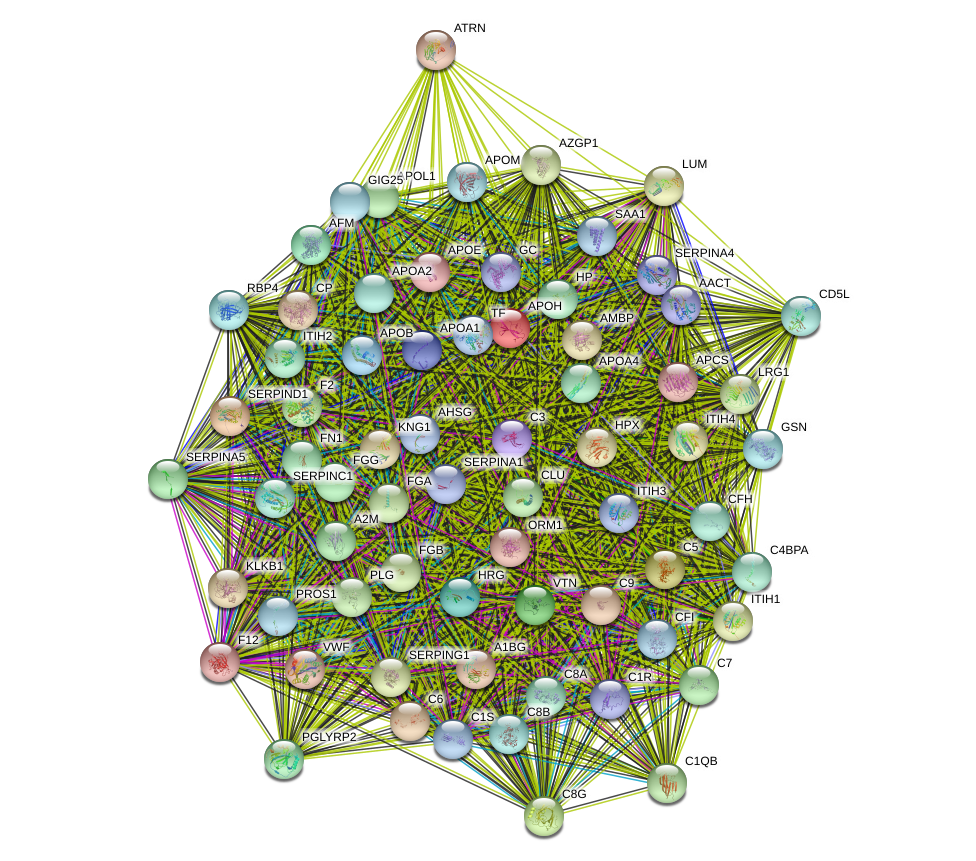
\includegraphics[width=1\linewidth]{figures/openms_protein_quantification/stringdb_plots/acute_c_improvers_vs_nonimprovers_run1_2021-03-23} \caption{The interaction network of differentially abundant proteins found in plasma 2-weeks post-injury, between AIS C patients who experienced an AIS grade conversion and those who did not. The coloured ``halo'' denotes fold change whereby green indicates that protein is less abundant and red indicates greater abundance. Edges represent protein-protein associations; these are known interactions from: curated databases 
\includegraphics[width=0.08\textwidth,height=0.02\textheight]{Images/stringdb_curated_db.png} and those that are experimentally determined 
\includegraphics[width=0.08\textwidth,height=0.02\textheight]{Images/stringdb_experimentally_determined.png}. Predicted interactions from: gene co-occurence 
\includegraphics[width=0.08\textwidth,height=0.02\textheight]{Images/stringdb_gene_co-occurrence.png}; gene fusions 
\includegraphics[width=0.08\textwidth,height=0.02\textheight]{Images/stringdb_gene_fusions.png}; gene neighbourhood 
\includegraphics[width=0.08\textwidth,height=0.02\textheight]{Images/stringdb_gene_neighbour.png}. Others are from gene co-expression 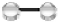
\includegraphics[width=0.08\textwidth,height=0.02\textheight]{Images/stringdb_co-expression.png}; text-mining 
\includegraphics[width=0.08\textwidth,height=0.02\textheight]{Images/stringdb_text_mining.png} and protein homology \includegraphics[width=0.08\textwidth,height=0.02\textheight]{Images/stringdb_protein-homology.png}.}\label{fig:openms-stringdb-acute-c-imp-vs-non}
\end{figure}



\begin{figure}
\includegraphics[width=1\linewidth]{figures/openms_protein_quantification/stringdb_plots/subacute_c_improvers_vs_nonimprovers_run1_2021-03-23} \caption{Interaction network of differentially abundant proteins from plasma 3-months post-injury, between AIS C patients who experienced an AIS grade conversion and those who did not. The coloured ``halo'' denotes fold change whereby green indicates that protein is less abundant and red that there is greater abundance. Edges represent protein-protein associations; these are known interactions from: curated databases \includegraphics[width=0.08\textwidth,height=0.02\textheight]{Images/stringdb_curated_db.png} and those that are experimentally determined \includegraphics[width=0.08\textwidth,height=0.02\textheight]{Images/stringdb_experimentally_determined.png}. Predicted interactions from: gene co-occurence \includegraphics[width=0.08\textwidth,height=0.02\textheight]{Images/stringdb_gene_co-occurrence.png}; gene fusions \includegraphics[width=0.08\textwidth,height=0.02\textheight]{Images/stringdb_gene_fusions.png}; gene neighbourhood \includegraphics[width=0.08\textwidth,height=0.02\textheight]{Images/stringdb_gene_neighbour.png}. Others are from gene co-expression \includegraphics[width=0.08\textwidth,height=0.02\textheight]{Images/stringdb_co-expression.png}; text-mining \includegraphics[width=0.08\textwidth,height=0.02\textheight]{Images/stringdb_text_mining.png} and protein homology \includegraphics[width=0.08\textwidth,height=0.02\textheight]{Images/stringdb_protein-homology.png}.}\label{fig:openms-stringdb-sub-cs}
\end{figure}



\begin{figure}
\includegraphics[width=1\linewidth]{figures/openms_protein_quantification/stringdb_plots/acute_c_improvers_vs_subacute_improvers_run1_2021-03-23} \caption[StringDB network plot - iTRAQ - Acute C Improvers VS Subacute Improvers]{Interaction network of differentially abundant proteins from plasma 2-weeks and 3-months post-injury for AIS C patients who experienced an AIS grade conversion. The coloured ``halo'' denotes fold change whereby green indicates that protein is less abundant and red that there is greater abundance. Edges represent protein-protein associations; these are known interactions from: curated databases \includegraphics[width=0.08\textwidth,height=0.02\textheight]{Images/stringdb_curated_db.png} and those that are experimentally determined \includegraphics[width=0.08\textwidth,height=0.02\textheight]{Images/stringdb_experimentally_determined.png}. Predicted interactions from: gene co-occurence \includegraphics[width=0.08\textwidth,height=0.02\textheight]{Images/stringdb_gene_co-occurrence.png}; gene fusions \includegraphics[width=0.08\textwidth,height=0.02\textheight]{Images/stringdb_gene_fusions.png}; gene neighbourhood \includegraphics[width=0.08\textwidth,height=0.02\textheight]{Images/stringdb_gene_neighbour.png}. Others are from gene co-expression \includegraphics[width=0.08\textwidth,height=0.02\textheight]{Images/stringdb_co-expression.png}; text-mining \includegraphics[width=0.08\textwidth,height=0.02\textheight]{Images/stringdb_text_mining.png} and protein homology \includegraphics[width=0.08\textwidth,height=0.02\textheight]{Images/stringdb_protein-homology.png}.}\label{fig:openms-stringdb-acute-sub-c-imp}
\end{figure}



\begin{figure}
\includegraphics[width=1\linewidth]{figures/openms_protein_quantification/stringdb_plots/acute_c_nonimprovers_vs_subacute_nonimprovers_run1_2021-03-23} \caption[StringDB network plot - iTRAQ - Acute C Non-Improvers VS Subacute Non-Improvers]{Interaction network of differentially abundant proteins from plasma 2-weeks and 3-months post-injury for AIS C patients who did not experience an AIS grade conversion. The coloured ``halo'' denotes fold change whereby green indicates that protein is less abundant and red that there is greater abundance. Edges represent protein-protein associations; these are known interactions from: curated databases \includegraphics[width=0.08\textwidth,height=0.02\textheight]{Images/stringdb_curated_db.png} and those that are experimentally determined \includegraphics[width=0.08\textwidth,height=0.02\textheight]{Images/stringdb_experimentally_determined.png}. Predicted interactions from: gene co-occurence \includegraphics[width=0.08\textwidth,height=0.02\textheight]{Images/stringdb_gene_co-occurrence.png}; gene fusions \includegraphics[width=0.08\textwidth,height=0.02\textheight]{Images/stringdb_gene_fusions.png}; gene neighbourhood \includegraphics[width=0.08\textwidth,height=0.02\textheight]{Images/stringdb_gene_neighbour.png}. Others are from gene co-expression \includegraphics[width=0.08\textwidth,height=0.02\textheight]{Images/stringdb_co-expression.png}; text-mining \includegraphics[width=0.08\textwidth,height=0.02\textheight]{Images/stringdb_text_mining.png} and protein homology \includegraphics[width=0.08\textwidth,height=0.02\textheight]{Images/stringdb_protein-homology.png}.}\label{fig:openms-stringdb-acute-sub-c-nonimp}
\end{figure}



\begin{figure}
\includegraphics[width=1\linewidth]{figures/openms_protein_quantification/stringdb_plots/a_vs_d_run2_2021-03-23} \caption[StringDB network plot - iTRAQ - Acute A VS Acute D]{Interaction network of differentially abundant proteins from plasma 2-week post-injury, between AIS A and D. The coloured ``halo'' denotes fold change whereby green indicates that protein is less abundant and red that there is greater abundance. Edges represent protein-protein associations; these are known interactions from: curated databases \includegraphics[width=0.08\textwidth,height=0.02\textheight]{Images/stringdb_curated_db.png} and those that are experimentally determined \includegraphics[width=0.08\textwidth,height=0.02\textheight]{Images/stringdb_experimentally_determined.png}. Predicted interactions from: gene co-occurence \includegraphics[width=0.08\textwidth,height=0.02\textheight]{Images/stringdb_gene_co-occurrence.png}; gene fusions \includegraphics[width=0.08\textwidth,height=0.02\textheight]{Images/stringdb_gene_fusions.png}; gene neighbourhood \includegraphics[width=0.08\textwidth,height=0.02\textheight]{Images/stringdb_gene_neighbour.png}. Others are from gene co-expression \includegraphics[width=0.08\textwidth,height=0.02\textheight]{Images/stringdb_co-expression.png}; text-mining \includegraphics[width=0.08\textwidth,height=0.02\textheight]{Images/stringdb_text_mining.png} and protein homology \includegraphics[width=0.08\textwidth,height=0.02\textheight]{Images/stringdb_protein-homology.png}.}\label{fig:openms-stringdb-a-vs-d}
\end{figure}



\begin{figure}
\includegraphics[width=1\linewidth]{figures/openms_protein_quantification/stringdb_plots/acute_c_improvers_vs_d_run2_2021-03-23} \caption[StringDB network plot - iTRAQ - Acute C Improvers VS Acute D]{Interaction network of differentially abundant proteins from plasma 2-week post-injury, between AIS C improvers and D. The coloured ``halo'' denotes fold change whereby green indicates that protein is less abundant and red that there is greater abundance. Edges represent protein-protein associations; these are known interactions from: curated databases \includegraphics[width=0.08\textwidth,height=0.02\textheight]{Images/stringdb_curated_db.png} and those that are experimentally determined \includegraphics[width=0.08\textwidth,height=0.02\textheight]{Images/stringdb_experimentally_determined.png}. Predicted interactions from: gene co-occurence \includegraphics[width=0.08\textwidth,height=0.02\textheight]{Images/stringdb_gene_co-occurrence.png}; gene fusions \includegraphics[width=0.08\textwidth,height=0.02\textheight]{Images/stringdb_gene_fusions.png}; gene neighbourhood \includegraphics[width=0.08\textwidth,height=0.02\textheight]{Images/stringdb_gene_neighbour.png}. Others are from gene co-expression \includegraphics[width=0.08\textwidth,height=0.02\textheight]{Images/stringdb_co-expression.png}; text-mining \includegraphics[width=0.08\textwidth,height=0.02\textheight]{Images/stringdb_text_mining.png} and protein homology \includegraphics[width=0.08\textwidth,height=0.02\textheight]{Images/stringdb_protein-homology.png}.}\label{fig:openms-stringdb-c-vs-d}
\end{figure}



\begin{figure}
\includegraphics[width=1\linewidth]{figures/openms_protein_quantification/stringdb_plots/acute_c_improvers_vs_a_run2_2021-03-23} \caption[StringDB network plot - iTRAQ - Acute C Improvers VS Acute A]{Interaction network of differentially abundant proteins from plasma 2-week post-injury, between AIS C improvers and A. The coloured ``halo'' denotes fold change whereby green indicates that protein is less abundant and red that there is greater abundance. Edges represent protein-protein associations; these are known interactions from: curated databases \includegraphics[width=0.08\textwidth,height=0.02\textheight]{Images/stringdb_curated_db.png} and those that are experimentally determined \includegraphics[width=0.08\textwidth,height=0.02\textheight]{Images/stringdb_experimentally_determined.png}. Predicted interactions from: gene co-occurence \includegraphics[width=0.08\textwidth,height=0.02\textheight]{Images/stringdb_gene_co-occurrence.png}; gene fusions \includegraphics[width=0.08\textwidth,height=0.02\textheight]{Images/stringdb_gene_fusions.png}; gene neighbourhood \includegraphics[width=0.08\textwidth,height=0.02\textheight]{Images/stringdb_gene_neighbour.png}. Others are from gene co-expression \includegraphics[width=0.08\textwidth,height=0.02\textheight]{Images/stringdb_co-expression.png}; text-mining \includegraphics[width=0.08\textwidth,height=0.02\textheight]{Images/stringdb_text_mining.png} and protein homology \includegraphics[width=0.08\textwidth,height=0.02\textheight]{Images/stringdb_protein-homology.png}.}\label{fig:openms-stringdb-c-vs-a}
\end{figure}



\begin{figure}
\includegraphics[width=1\linewidth]{figures/openms_protein_quantification/stringdb_plots/acute_c_nonimprovers_vs_a_run2_2021-03-23} \caption[StringDB network plot - iTRAQ - Acute C Non-Improvers VS Acute A]{Interaction network of differentially abundant proteins from plasma 2-week post-injury, between AIS C non-improvers and A. The coloured ``halo'' denotes fold change whereby green indicates that protein is less abundant and red that there is greater abundance. Edges represent protein-protein associations; these are known interactions from: curated databases \includegraphics[width=0.08\textwidth,height=0.02\textheight]{Images/stringdb_curated_db.png} and those that are experimentally determined \includegraphics[width=0.08\textwidth,height=0.02\textheight]{Images/stringdb_experimentally_determined.png}. Predicted interactions from: gene co-occurence \includegraphics[width=0.08\textwidth,height=0.02\textheight]{Images/stringdb_gene_co-occurrence.png}; gene fusions \includegraphics[width=0.08\textwidth,height=0.02\textheight]{Images/stringdb_gene_fusions.png}; gene neighbourhood \includegraphics[width=0.08\textwidth,height=0.02\textheight]{Images/stringdb_gene_neighbour.png}. Others are from gene co-expression \includegraphics[width=0.08\textwidth,height=0.02\textheight]{Images/stringdb_co-expression.png}; text-mining \includegraphics[width=0.08\textwidth,height=0.02\textheight]{Images/stringdb_text_mining.png} and protein homology \includegraphics[width=0.08\textwidth,height=0.02\textheight]{Images/stringdb_protein-homology.png}.}\label{fig:openms-stringdb-c-nonimp-vs-a}
\end{figure}



\begin{figure}
\includegraphics[width=1\linewidth]{figures/openms_protein_quantification/stringdb_plots/acute_c_nonimprovers_vs_d_run2_2021-03-23} \caption[StringDB network plot - iTRAQ - Acute C Non-Improvers VS Acute D]{Interaction network of differentially abundant proteins from plasma 2-week post-injury, between AIS C non-improvers and D. The coloured ``halo'' denotes fold change whereby green indicates that protein is less abundant and red that there is greater abundance. Edges represent protein-protein associations; these are known interactions from: curated databases \includegraphics[width=0.08\textwidth,height=0.02\textheight]{Images/stringdb_curated_db.png} and those that are experimentally determined \includegraphics[width=0.08\textwidth,height=0.02\textheight]{Images/stringdb_experimentally_determined.png}. Predicted interactions from: gene co-occurence \includegraphics[width=0.08\textwidth,height=0.02\textheight]{Images/stringdb_gene_co-occurrence.png}; gene fusions \includegraphics[width=0.08\textwidth,height=0.02\textheight]{Images/stringdb_gene_fusions.png}; gene neighbourhood \includegraphics[width=0.08\textwidth,height=0.02\textheight]{Images/stringdb_gene_neighbour.png}. Others are from gene co-expression \includegraphics[width=0.08\textwidth,height=0.02\textheight]{Images/stringdb_co-expression.png}; text-mining \includegraphics[width=0.08\textwidth,height=0.02\textheight]{Images/stringdb_text_mining.png} and protein homology \includegraphics[width=0.08\textwidth,height=0.02\textheight]{Images/stringdb_protein-homology.png}.}\label{fig:openms-stringdb-c-nonimp-vs-d}
\end{figure}

\hypertarget{label-free-data-2}{%
\subsubsection{Label-free data}\label{label-free-data-2}}



\begin{figure}
\includegraphics[width=1\linewidth]{figures/openms_protein_quantification/label_free/stringdb_plots/acute_c_imp_vs_acute_c_nonimp_2021-08-06} \caption{The interaction network of differentially abundant proteins found in plasma 2-weeks post-injury, between AIS C patients who experienced an AIS grade conversion and those who did not. The coloured ``halo'' denotes fold change whereby green indicates that protein is less abundant and red indicates greater abundance. Edges represent protein-protein associations; these are known interactions from: curated databases \includegraphics[width=0.08\textwidth,height=0.02\textheight]{Images/stringdb_curated_db.png} and those that are experimentally determined \includegraphics[width=0.08\textwidth,height=0.02\textheight]{Images/stringdb_experimentally_determined.png}. Predicted interactions from: gene co-occurence \includegraphics[width=0.08\textwidth,height=0.02\textheight]{Images/stringdb_gene_co-occurrence.png}; gene fusions \includegraphics[width=0.08\textwidth,height=0.02\textheight]{Images/stringdb_gene_fusions.png}; gene neighbourhood \includegraphics[width=0.08\textwidth,height=0.02\textheight]{Images/stringdb_gene_neighbour.png}. Others are from gene co-expression \includegraphics[width=0.08\textwidth,height=0.02\textheight]{Images/stringdb_co-expression.png}; text-mining \includegraphics[width=0.08\textwidth,height=0.02\textheight]{Images/stringdb_text_mining.png} and protein homology \includegraphics[width=0.08\textwidth,height=0.02\textheight]{Images/stringdb_protein-homology.png}.}\label{fig:openms-stringdb-chap4-acute-c-imp-vs-nonimp}
\end{figure}



\begin{figure}
\includegraphics[width=1\linewidth]{figures/openms_protein_quantification/label_free/stringdb_plots/subacute_c_imp_vs_subacute_c_nonimp_2021-08-06} \caption{Interaction network of differentially abundant proteins from plasma 3-months post-injury, between AIS C patients who experienced an AIS grade conversion and those who did not. The coloured ``halo'' denotes fold change whereby green indicates that protein is less abundant and red that there is greater abundance. Edges represent protein-protein associations; these are known interactions from: curated databases \includegraphics[width=0.08\textwidth,height=0.02\textheight]{Images/stringdb_curated_db.png} and those that are experimentally determined \includegraphics[width=0.08\textwidth,height=0.02\textheight]{Images/stringdb_experimentally_determined.png}. Predicted interactions from: gene co-occurence \includegraphics[width=0.08\textwidth,height=0.02\textheight]{Images/stringdb_gene_co-occurrence.png}; gene fusions \includegraphics[width=0.08\textwidth,height=0.02\textheight]{Images/stringdb_gene_fusions.png}; gene neighbourhood \includegraphics[width=0.08\textwidth,height=0.02\textheight]{Images/stringdb_gene_neighbour.png}. Others are from gene co-expression \includegraphics[width=0.08\textwidth,height=0.02\textheight]{Images/stringdb_co-expression.png}; text-mining \includegraphics[width=0.08\textwidth,height=0.02\textheight]{Images/stringdb_text_mining.png} and protein homology \includegraphics[width=0.08\textwidth,height=0.02\textheight]{Images/stringdb_protein-homology.png}.}\label{fig:openms-stringdb-chap4-sub-cs}
\end{figure}





\begin{figure}
\includegraphics[width=1\linewidth]{figures/openms_protein_quantification/label_free/stringdb_plots/acute_c_imp_vs_subacute_c_imp_2021-08-06} \caption[StringDB network plot - label-free - Acute C Improvers VS Subacute Improvers]{Interaction network of differentially abundant proteins from plasma 2-weeks and 3-months post-injury for AIS C patients who experienced an AIS grade conversion. The coloured ``halo'' denotes fold change whereby green indicates that protein is less abundant and red that there is greater abundance. Edges represent protein-protein associations; these are known interactions from: curated databases \includegraphics[width=0.08\textwidth,height=0.02\textheight]{Images/stringdb_curated_db.png} and those that are experimentally determined \includegraphics[width=0.08\textwidth,height=0.02\textheight]{Images/stringdb_experimentally_determined.png}. Predicted interactions from: gene co-occurence \includegraphics[width=0.08\textwidth,height=0.02\textheight]{Images/stringdb_gene_co-occurrence.png}; gene fusions \includegraphics[width=0.08\textwidth,height=0.02\textheight]{Images/stringdb_gene_fusions.png}; gene neighbourhood \includegraphics[width=0.08\textwidth,height=0.02\textheight]{Images/stringdb_gene_neighbour.png}. Others are from gene co-expression \includegraphics[width=0.08\textwidth,height=0.02\textheight]{Images/stringdb_co-expression.png}; text-mining \includegraphics[width=0.08\textwidth,height=0.02\textheight]{Images/stringdb_text_mining.png} and protein homology \includegraphics[width=0.08\textwidth,height=0.02\textheight]{Images/stringdb_protein-homology.png}.}\label{fig:openms-stringdb-chap4-acute-sub-c-imp}
\end{figure}



\begin{figure}
\includegraphics[width=1\linewidth]{figures/openms_protein_quantification/label_free/stringdb_plots/acute_c_nonimp_vs_subacute_c_nonimp_2021-08-06} \caption[StringDB network plot - label-free - Acute C Non-Improvers VS Subacute Non-Improvers]{Interaction network of differentially abundant proteins from plasma 2-weeks and 3-months post-injury for AIS C patients who did not experience an AIS grade conversion. The coloured ``halo'' denotes fold change whereby green indicates that protein is less abundant and red that there is greater abundance. Edges represent protein-protein associations; these are known interactions from: curated databases \includegraphics[width=0.08\textwidth,height=0.02\textheight]{Images/stringdb_curated_db.png} and those that are experimentally determined \includegraphics[width=0.08\textwidth,height=0.02\textheight]{Images/stringdb_experimentally_determined.png}. Predicted interactions from: gene co-occurence \includegraphics[width=0.08\textwidth,height=0.02\textheight]{Images/stringdb_gene_co-occurrence.png}; gene fusions \includegraphics[width=0.08\textwidth,height=0.02\textheight]{Images/stringdb_gene_fusions.png}; gene neighbourhood \includegraphics[width=0.08\textwidth,height=0.02\textheight]{Images/stringdb_gene_neighbour.png}. Others are from gene co-expression \includegraphics[width=0.08\textwidth,height=0.02\textheight]{Images/stringdb_co-expression.png}; text-mining \includegraphics[width=0.08\textwidth,height=0.02\textheight]{Images/stringdb_text_mining.png} and protein homology \includegraphics[width=0.08\textwidth,height=0.02\textheight]{Images/stringdb_protein-homology.png}.}\label{fig:openms-stringdb-chap4-acute-sub-c-nonimp}
\end{figure}



\begin{figure}
\includegraphics[width=1\linewidth]{figures/openms_protein_quantification/label_free/stringdb_plots/acute_a_vs_acute_d_2021-08-06} \caption[StringDB network plot - label-free - Acute A VS Acute D]{Interaction network of differentially abundant proteins from plasma 2-week post-injury, between AIS A and D. The coloured ``halo'' denotes fold change whereby green indicates that protein is less abundant and red that there is greater abundance. Edges represent protein-protein associations; these are known interactions from: curated databases \includegraphics[width=0.08\textwidth,height=0.02\textheight]{Images/stringdb_curated_db.png} and those that are experimentally determined \includegraphics[width=0.08\textwidth,height=0.02\textheight]{Images/stringdb_experimentally_determined.png}. Predicted interactions from: gene co-occurence \includegraphics[width=0.08\textwidth,height=0.02\textheight]{Images/stringdb_gene_co-occurrence.png}; gene fusions \includegraphics[width=0.08\textwidth,height=0.02\textheight]{Images/stringdb_gene_fusions.png}; gene neighbourhood \includegraphics[width=0.08\textwidth,height=0.02\textheight]{Images/stringdb_gene_neighbour.png}. Others are from gene co-expression \includegraphics[width=0.08\textwidth,height=0.02\textheight]{Images/stringdb_co-expression.png}; text-mining \includegraphics[width=0.08\textwidth,height=0.02\textheight]{Images/stringdb_text_mining.png} and protein homology \includegraphics[width=0.08\textwidth,height=0.02\textheight]{Images/stringdb_protein-homology.png}.}\label{fig:openms-stringdb-chap4-a-vs-d}
\end{figure}



\begin{figure}
\includegraphics[width=1\linewidth]{figures/openms_protein_quantification/label_free/stringdb_plots/acute_c_imp_vs_acute_d_2021-08-06} \caption[StringDB network plot - label-free - Acute C Improvers VS Acute D]{Interaction network of differentially abundant proteins from plasma 2-week post-injury, between AIS C improvers and D. The coloured ``halo'' denotes fold change whereby green indicates that protein is less abundant and red that there is greater abundance. Edges represent protein-protein associations; these are known interactions from: curated databases \includegraphics[width=0.08\textwidth,height=0.02\textheight]{Images/stringdb_curated_db.png} and those that are experimentally determined \includegraphics[width=0.08\textwidth,height=0.02\textheight]{Images/stringdb_experimentally_determined.png}. Predicted interactions from: gene co-occurence \includegraphics[width=0.08\textwidth,height=0.02\textheight]{Images/stringdb_gene_co-occurrence.png}; gene fusions \includegraphics[width=0.08\textwidth,height=0.02\textheight]{Images/stringdb_gene_fusions.png}; gene neighbourhood \includegraphics[width=0.08\textwidth,height=0.02\textheight]{Images/stringdb_gene_neighbour.png}. Others are from gene co-expression \includegraphics[width=0.08\textwidth,height=0.02\textheight]{Images/stringdb_co-expression.png}; text-mining \includegraphics[width=0.08\textwidth,height=0.02\textheight]{Images/stringdb_text_mining.png} and protein homology \includegraphics[width=0.08\textwidth,height=0.02\textheight]{Images/stringdb_protein-homology.png}.}\label{fig:openms-stringdb-chap4-c-vs-d}
\end{figure}



\begin{figure}
\includegraphics[width=1\linewidth]{figures/openms_protein_quantification/label_free/stringdb_plots/acute_a_vs_acute_c_imp_2021-08-06} \caption[StringDB network plot - label-free - Acute C Improvers VS Acute A]{Interaction network of differentially abundant proteins from plasma 2-week post-injury, between AIS C improvers and A. The coloured ``halo'' denotes fold change whereby green indicates that protein is less abundant and red that there is greater abundance. Edges represent protein-protein associations; these are known interactions from: curated databases \includegraphics[width=0.08\textwidth,height=0.02\textheight]{Images/stringdb_curated_db.png} and those that are experimentally determined \includegraphics[width=0.08\textwidth,height=0.02\textheight]{Images/stringdb_experimentally_determined.png}. Predicted interactions from: gene co-occurence \includegraphics[width=0.08\textwidth,height=0.02\textheight]{Images/stringdb_gene_co-occurrence.png}; gene fusions \includegraphics[width=0.08\textwidth,height=0.02\textheight]{Images/stringdb_gene_fusions.png}; gene neighbourhood \includegraphics[width=0.08\textwidth,height=0.02\textheight]{Images/stringdb_gene_neighbour.png}. Others are from gene co-expression \includegraphics[width=0.08\textwidth,height=0.02\textheight]{Images/stringdb_co-expression.png}; text-mining \includegraphics[width=0.08\textwidth,height=0.02\textheight]{Images/stringdb_text_mining.png} and protein homology \includegraphics[width=0.08\textwidth,height=0.02\textheight]{Images/stringdb_protein-homology.png}.}\label{fig:openms-stringdb-chap4-c-vs-a}
\end{figure}



\begin{figure}
\includegraphics[width=1\linewidth]{figures/openms_protein_quantification/label_free/stringdb_plots/acute_a_vs_acute_c_nonimp_2021-08-06} \caption[StringDB network plot - label-free - Acute C Non-Improvers VS Acute A]{Interaction network of differentially abundant proteins from plasma 2-week post-injury, between AIS C non-improvers and A. The coloured ``halo'' denotes fold change whereby green indicates that protein is less abundant and red that there is greater abundance. Edges represent protein-protein associations; these are known interactions from: curated databases \includegraphics[width=0.08\textwidth,height=0.02\textheight]{Images/stringdb_curated_db.png} and those that are experimentally determined \includegraphics[width=0.08\textwidth,height=0.02\textheight]{Images/stringdb_experimentally_determined.png}. Predicted interactions from: gene co-occurence \includegraphics[width=0.08\textwidth,height=0.02\textheight]{Images/stringdb_gene_co-occurrence.png}; gene fusions \includegraphics[width=0.08\textwidth,height=0.02\textheight]{Images/stringdb_gene_fusions.png}; gene neighbourhood \includegraphics[width=0.08\textwidth,height=0.02\textheight]{Images/stringdb_gene_neighbour.png}. Others are from gene co-expression \includegraphics[width=0.08\textwidth,height=0.02\textheight]{Images/stringdb_co-expression.png}; text-mining \includegraphics[width=0.08\textwidth,height=0.02\textheight]{Images/stringdb_text_mining.png} and protein homology \includegraphics[width=0.08\textwidth,height=0.02\textheight]{Images/stringdb_protein-homology.png}.}\label{fig:openms-stringdb-chap4-c-nonimp-vs-a}
\end{figure}



\begin{figure}
\includegraphics[width=1\linewidth]{figures/openms_protein_quantification/label_free/stringdb_plots/acute_c_nonimp_vs_acute_d_2021-08-06} \caption[StringDB network plot - label-free - Acute C Non-Improvers VS Acute D]{Interaction network of differentially abundant proteins from plasma 2-week post-injury, between AIS C non-improvers and D. The coloured ``halo'' denotes fold change whereby green indicates that protein is less abundant and red that there is greater abundance. Edges represent protein-protein associations; these are known interactions from: curated databases \includegraphics[width=0.08\textwidth,height=0.02\textheight]{Images/stringdb_curated_db.png} and those that are experimentally determined \includegraphics[width=0.08\textwidth,height=0.02\textheight]{Images/stringdb_experimentally_determined.png}. Predicted interactions from: gene co-occurence \includegraphics[width=0.08\textwidth,height=0.02\textheight]{Images/stringdb_gene_co-occurrence.png}; gene fusions \includegraphics[width=0.08\textwidth,height=0.02\textheight]{Images/stringdb_gene_fusions.png}; gene neighbourhood \includegraphics[width=0.08\textwidth,height=0.02\textheight]{Images/stringdb_gene_neighbour.png}. Others are from gene co-expression \includegraphics[width=0.08\textwidth,height=0.02\textheight]{Images/stringdb_co-expression.png}; text-mining \includegraphics[width=0.08\textwidth,height=0.02\textheight]{Images/stringdb_text_mining.png} and protein homology \includegraphics[width=0.08\textwidth,height=0.02\textheight]{Images/stringdb_protein-homology.png}.}\label{fig:openms-stringdb-chap4-c-nonimp-vs-d}
\end{figure}

\clearpage

\hypertarget{sup-volc-plots}{%
\subsection{Volcano plots}\label{sup-volc-plots}}



\begin{figure}
\includegraphics[width=1\linewidth]{figures/openms_protein_quantification/label_free/volcano_plots/openms_volcano_plot_2021-08-10_0008} \caption{Volcano plot of log\(_10\) fold change and log\(_10\) adjusted p-value for plasma proteins from 2-weeks post-injury between AIS C patients who experienced an AIS grade conversion and those who did not. Proteins with a fold changes beyond \(\pm 1.2\) and an adjusted p-value less than 0.05 are labelled.}\label{fig:volc-plot-c-imp-vs-nonimp}
\end{figure}



\begin{figure}
\includegraphics[width=1\linewidth]{figures/openms_protein_quantification/label_free/volcano_plots/openms_volcano_plot_2021-08-10_0026} \caption{Volcano plot of log\(_10\) fold change and log\(_10\) adjusted p-value for plasma proteins from 3-months post-injury between AIS C patients who experienced an AIS grade conversion and those who did not. Proteins with a fold changes beyond \(\pm 1.2\) and an adjusted p-value less than 0.05 are labelled.}\label{fig:volc-plot-subacute-c-imp-vs-nonimp}
\end{figure}



\begin{figure}
\includegraphics[width=1\linewidth]{figures/openms_protein_quantification/label_free/volcano_plots/openms_volcano_plot_2021-08-10_0011} \caption{Volcano plot of log\(_10\) fold change and log\(_10\) adjusted p-value for plasma proteins from 2-weeks and 3-months post-injury from AIS C patients who experienced an AIS grade conversion. Proteins with a fold changes beyond \(\pm 1.2\) and an adjusted p-value less than 0.05 are labelled.}\label{fig:volc-plot-acute-c-imp-vs-subacute-imp}
\end{figure}



\begin{figure}
\includegraphics[width=1\linewidth]{figures/openms_protein_quantification/label_free/volcano_plots/openms_volcano_plot_2021-08-10_0017} \caption{Volcano plot of log\(_10\) fold change and log\(_10\) adjusted p-value for plasma proteins from 2-weeks and 3-months post-injury from AIS C patients who did not experience an AIS grade conversion. Proteins with a fold changes beyond \(\pm 1.2\) and an adjusted p-value less than 0.05 are labelled.}\label{fig:volc-plot-acute-c-nonimp-vs-subacute-nonimp}
\end{figure}



\begin{figure}
\includegraphics[width=1\linewidth]{figures/openms_protein_quantification/label_free/volcano_plots/openms_volcano_plot_2021-08-10_0003} \caption{Volcano plot of log\(_10\) fold change and log\(_10\) adjusted p-value for plasma proteins from 2-weeks post-injury between AIS A and AIS D patients. Proteins with a fold changes beyond \(\pm 1.2\) and an adjusted p-value less than 0.05 are labelled.}\label{fig:volc-plot-acute-a-vs-acute-d}
\end{figure}



\begin{figure}
\includegraphics[width=1\linewidth]{figures/openms_protein_quantification/label_free/volcano_plots/openms_volcano_plot_2021-08-10_0004} \caption{Volcano plot of log\(_10\) fold change and log\(_10\) adjusted p-value for plasma proteins from 2-weeks and 3-months post-injury from AIS A patients. Proteins with a fold changes beyond \(\pm 1.2\) and an adjusted p-value less than 0.05 are labelled.}\label{fig:volc-plot-acute-a-vs-subacute-a}
\end{figure}



\begin{figure}
\includegraphics[width=1\linewidth]{figures/openms_protein_quantification/label_free/volcano_plots/openms_volcano_plot_2021-08-10_0022} \caption{Volcano plot of log\(_10\) fold change and log\(_10\) adjusted p-value for plasma proteins from 2-weeks and 3-months post-injury from AIS D patients. Proteins with a fold changes beyond \(\pm 1.2\) and an adjusted p-value less than 0.05 are labelled.}\label{fig:volc-plot-acute-d-vs-subacute-d}
\end{figure}



\begin{figure}
\includegraphics[width=1\linewidth]{figures/openms_protein_quantification/label_free/volcano_plots/openms_volcano_plot_2021-08-10_0009} \caption{Volcano plot of log\(_10\) fold change and log\(_10\) adjusted p-value for plasma proteins from 2-weeks post-injury between AIS C patients who experienced an AIS grade conversion and AIS D patients. Proteins with a fold changes beyond \(\pm 1.2\) and an adjusted p-value less than 0.05 are labelled.}\label{fig:volc-plot-acute-c-imp-vs-acute-d}
\end{figure}



\begin{figure}
\includegraphics[width=1\linewidth]{figures/openms_protein_quantification/label_free/volcano_plots/openms_volcano_plot_2021-08-10_0001} \caption{Volcano plot of log\(_10\) fold change and log\(_10\) adjusted p-value for plasma proteins from 2-weeks post-injury between AIS A patients and AIS C patients who experienced an AIS grade conversion. Proteins with a fold changes beyond \(\pm 1.2\) and an adjusted p-value less than 0.05 are labelled.}\label{fig:volc-plot-acute-a-vs-acute-c-imp}
\end{figure}



\begin{figure}
\includegraphics[width=1\linewidth]{figures/openms_protein_quantification/label_free/volcano_plots/openms_volcano_plot_2021-08-10_0002} \caption{Volcano plot of log\(_10\) fold change and log\(_10\) adjusted p-value for plasma proteins from 2-weeks post-injury between AIS A patients and AIS C patients who did not experience an AIS grade conversion. Proteins with a fold changes beyond \(\pm 1.2\) and an adjusted p-value less than 0.05 are labelled.}\label{fig:volc-plot-acute-a-vs-acute-c-nonimp}
\end{figure}



\begin{figure}
\includegraphics[width=1\linewidth]{figures/openms_protein_quantification/label_free/volcano_plots/openms_volcano_plot_2021-08-10_0014} \caption{Volcano plot of log\(_10\) fold change and log\(_10\) adjusted p-value for plasma proteins from 2-weeks post-injury between AIS C patients who did not experience an AIS grade conversion and AIS D patients. Proteins with a fold changes beyond \(\pm 1.2\) and an adjusted p-value less than 0.05 are labelled.}\label{fig:volc-plot-acute-c-nonimp-vs-acute-d}
\end{figure}

\hypertarget{references}{%
\section*{References}\label{references}}
\addcontentsline{toc}{section}{References}

\hypertarget{refs}{}
\begin{CSLReferences}{1}{0}
\leavevmode\vadjust pre{\hypertarget{ref-ahuja_traumatic_2017}{}}%
Ahuja, Christopher S, Jefferson R Wilson, Satoshi Nori, Mark R N Kotter, Claudia Druschel, Armin Curt, and Michael G Fehlings. 2017. {``Traumatic Spinal Cord Injury.''} \emph{Nat Rev Dis Primers} 3: 17018. \url{https://doi.org/10.1038/nrdp.2017.18}.

\leavevmode\vadjust pre{\hypertarget{ref-altznauer_concurrent_2003}{}}%
Altznauer, Frank, Stephan von Gunten, Peter Späth, and Hans-Uwe Simon. 2003. {``Concurrent Presence of Agonistic and Antagonistic Anti-{Cd95} Autoantibodies in Intravenous {Ig} Preparations.''} \emph{Journal of Allergy and Clinical Immunology} 112 (6): 1185--90. \url{https://doi.org/10.1016/j.jaci.2003.09.045}.

\leavevmode\vadjust pre{\hypertarget{ref-anatol_small_2003}{}}%
Anatol, Kontush, Chantepie Sandrine, and Chapman M. John. 2003. {``Small, {Dense HDL Particles Exert Potent Protection} of {Atherogenic LDL Against Oxidative Stress}.''} \emph{Arteriosclerosis, Thrombosis, and Vascular Biology} 23 (10): 1881--88. \url{https://doi.org/10.1161/01.ATV.0000091338.93223.E8}.

\leavevmode\vadjust pre{\hypertarget{ref-anderson_astrocyte_2016}{}}%
Anderson, Mark A., Joshua E. Burda, Yilong Ren, Yan Ao, Timothy M. O'Shea, Riki Kawaguchi, Giovanni Coppola, Baljit S. Khakh, Timothy J. Deming, and Michael V. Sofroniew. 2016. {``Astrocyte Scar Formation Aids Central Nervous System Axon Regeneration.''} \emph{Nature} 532 (7598): 195--200. \url{https://doi.org/10.1038/nature17623}.

\leavevmode\vadjust pre{\hypertarget{ref-ankeny_b_2009}{}}%
Ankeny, Daniel P., Zhen Guan, and Phillip G. Popovich. 2009. {``B Cells Produce Pathogenic Antibodies and Impair Recovery After Spinal Cord Injury in Mice.''} \emph{The Journal of Clinical Investigation} 119 (10): 2990--99. \url{https://doi.org/10.1172/JCI39780}.

\leavevmode\vadjust pre{\hypertarget{ref-anthony_systemic_2014}{}}%
Anthony, Daniel C., and Yvonne Couch. 2014. {``The Systemic Response to {CNS} Injury.''} \emph{Experimental Neurology}, Special {Issue}: {Neuroimmunology} of spinal cord injury, 258 (August): 105--11. \url{https://doi.org/10.1016/j.expneurol.2014.03.013}.

\leavevmode\vadjust pre{\hypertarget{ref-arevalo-martin_elevated_2018}{}}%
Arevalo-Martin, Angel, Lukas Grassner, Daniel Garcia-Ovejero, Beatriz Paniagua-Torija, Gemma Barroso-Garcia, Alba G. Arandilla, Orpheus Mach, et al. 2018. {``Elevated {Autoantibodies} in {Subacute Human Spinal Cord Injury Are Naturally Occurring Antibodies}.''} \emph{Frontiers in Immunology} 9: 2365. \url{https://doi.org/10.3389/fimmu.2018.02365}.

\leavevmode\vadjust pre{\hypertarget{ref-arpaia_metabolites_2013}{}}%
Arpaia, Nicholas, Clarissa Campbell, Xiying Fan, Stanislav Dikiy, Joris van der Veeken, Paul deRoos, Hui Liu, et al. 2013. {``Metabolites Produced by Commensal Bacteria Promote Peripheral Regulatory {T-cell} Generation.''} \emph{Nature} 504 (7480): 451--55. \url{https://doi.org/10.1038/nature12726}.

\leavevmode\vadjust pre{\hypertarget{ref-arumugam_intravenous_2007}{}}%
Arumugam, Thiruma V., Sung-Chun Tang, Justin D. Lathia, Aiwu Cheng, Mohamed R. Mughal, Srinivasulu Chigurupati, Tim Magnus, et al. 2007. {``Intravenous Immunoglobulin ({IVIG}) Protects the Brain Against Experimental Stroke by Preventing Complement-Mediated Neuronal Cell Death.''} \emph{Proceedings of the National Academy of Sciences of the United States of America} 104 (35): 14104--9. \url{https://doi.org/10.1073/pnas.0700506104}.

\leavevmode\vadjust pre{\hypertarget{ref-balmer_gene_2002}{}}%
Balmer, James E., and Rune Blomhoff. 2002. {``Gene Expression Regulation by Retinoic Acid.''} \emph{Journal of Lipid Research} 43 (11): 1773--1808. \url{https://doi.org/10.1194/jlr.R100015-JLR200}.

\leavevmode\vadjust pre{\hypertarget{ref-balmer_liver_2014}{}}%
Balmer, Maria L., Emma Slack, Andrea de Gottardi, Melissa A. E. Lawson, Siegfried Hapfelmeier, Luca Miele, Antonio Grieco, et al. 2014. {``The {Liver May Act} as a {Firewall Mediating Mutualism Between} the {Host} and {Its Gut Commensal Microbiota}.''} \emph{Science Translational Medicine} 6 (237): 237ra66--66. \url{https://doi.org/10.1126/scitranslmed.3008618}.

\leavevmode\vadjust pre{\hypertarget{ref-balzan_bacterial_2007}{}}%
Balzan, Silvio, Claudio De Almeida Quadros, Roberto De Cleva, Bruno Zilberstein, and Ivan Cecconello. 2007. {``Bacterial Translocation: {Overview} of Mechanisms and Clinical Impact.''} \emph{Journal of Gastroenterology and Hepatology} 22 (4): 464--71. \url{https://doi.org/10.1111/j.1440-1746.2007.04933.x}.

\leavevmode\vadjust pre{\hypertarget{ref-banka_serum_1995}{}}%
Banka, C. L., T. Yuan, M. C. de Beer, M. Kindy, L. K. Curtiss, and F. C. de Beer. 1995. {``\href{https://www.ncbi.nlm.nih.gov/pubmed/7658153}{Serum Amyloid {A} ({SAA}): Influence on {HDL-mediated} Cellular Cholesterol Efflux.}''} \emph{Journal of Lipid Research} 36 (5): 1058--65.

\leavevmode\vadjust pre{\hypertarget{ref-bao_systemic_2012}{}}%
Bao, Feng, Vanessa Omana, Arthur Brown, and Lynne C. Weaver. 2012. {``The Systemic Inflammatory Response After Spinal Cord Injury in the Rat Is Decreased by {a4B1} Integrin Blockade.''} \emph{Journal of Neurotrauma} 29 (8): 1626--37. \url{https://doi.org/10.1089/neu.2011.2190}.

\leavevmode\vadjust pre{\hypertarget{ref-basta_fab2-mediated_2003}{}}%
Basta, Milan, Fredric Van Goor, Stefano Luccioli, Eric M. Billings, Alexander O. Vortmeyer, Lajos Baranyi, Janos Szebeni, et al. 2003. {``F(ab){\({'}\)}2-Mediated Neutralization of {C3a} and {C5a} Anaphylatoxins: A Novel Effector Function of Immunoglobulins.''} \emph{Nature Medicine} 9 (4): 431--38. \url{https://doi.org/10.1038/nm836}.

\leavevmode\vadjust pre{\hypertarget{ref-basta_mechanism_1989}{}}%
Basta, M, P Kirshbom, M M Frank, and L F Fries. 1989. {``Mechanism of Therapeutic Effect of High-Dose Intravenous Immunoglobulin. {Attenuation} of Acute, Complement-Dependent Immune Damage in a Guinea Pig Model.''} \emph{Journal of Clinical Investigation} 84 (6): 1974--81. \url{https://doi.org/10.1172/JCI114387}.

\leavevmode\vadjust pre{\hypertarget{ref-bastien_il-1_2015}{}}%
Bastien, Dominic, Victor Bellver Landete, Martine Lessard, Nicolas Vallières, Mathieu Champagne, Akira Takashima, Marie-Ève Tremblay, Yannick Doyon, and Steve Lacroix. 2015. {``{IL-1\(\alpha\) Gene Deletion Protects Oligodendrocytes} After {Spinal Cord Injury} Through {Upregulation} of the {Survival Factor Tox3}.''} \emph{The Journal of Neuroscience} 35 (30): 10715--30. \url{https://doi.org/10.1523/JNEUROSCI.0498-15.2015}.

\leavevmode\vadjust pre{\hypertarget{ref-bastien_cytokine_2014}{}}%
Bastien, Dominic, and Steve Lacroix. 2014. {``Cytokine Pathways Regulating Glial and Leukocyte Function After Spinal Cord and Peripheral Nerve Injury.''} \emph{Experimental Neurology}, Special {Issue}: {Neuroimmunology} of spinal cord injury, 258 (August): 62--77. \url{https://doi.org/10.1016/j.expneurol.2014.04.006}.

\leavevmode\vadjust pre{\hypertarget{ref-bauman_carbohydrate_2001}{}}%
Bauman, William A., and Ann M. Spungen. 2001. {``Carbohydrate {And Lipid Metabolism In Chronic Spinal Cord Injury}.''} \emph{The Journal of Spinal Cord Medicine} 24 (4): 266--77. \url{https://doi.org/10.1080/10790268.2001.11753584}.

\leavevmode\vadjust pre{\hypertarget{ref-bayry_intravenous_2011}{}}%
Bayry, Jagadeesh, Vir Singh Negi, and Srini V. Kaveri. 2011. {``Intravenous Immunoglobulin Therapy in Rheumatic Diseases.''} \emph{Nature Reviews Rheumatology} 7 (6): 349--59. \url{https://doi.org/10.1038/nrrheum.2011.61}.

\leavevmode\vadjust pre{\hypertarget{ref-bazzocchi_changes_2021}{}}%
Bazzocchi, Gabriele, Silvia Turroni, Maria Chiara Bulzamini, Federica D'Amico, Angelica Bava, Mirco Castiglioni, Valentina Cagnetta, et al. 2021. {``Changes in Gut Microbiota in the Acute Phase After Spinal Cord Injury Correlate with Severity of the Lesion.''} \emph{Scientific Reports} 11 (1): 12743. \url{https://doi.org/10.1038/s41598-021-92027-z}.

\leavevmode\vadjust pre{\hypertarget{ref-beck_quantitative_2010}{}}%
Beck, Kevin D., Hal X. Nguyen, Manuel D. Galvan, Desirée L. Salazar, Trent M. Woodruff, and Aileen J. Anderson. 2010. {``Quantitative Analysis of Cellular Inflammation After Traumatic Spinal Cord Injury: Evidence for a Multiphasic Inflammatory Response in the Acute to Chronic Environment.''} \emph{Brain} 133 (2): 433--47. \url{https://doi.org/10.1093/brain/awp322}.

\leavevmode\vadjust pre{\hypertarget{ref-bellver-landete_microglia_2019}{}}%
Bellver-Landete, Victor, Floriane Bretheau, Benoit Mailhot, Nicolas Vallières, Martine Lessard, Marie-Eve Janelle, Nathalie Vernoux, et al. 2019. {``Microglia Are an Essential Component of the Neuroprotective Scar That Forms After Spinal Cord Injury.''} \emph{Nature Communications} 10 (1): 518. \url{https://doi.org/10.1038/s41467-019-08446-0}.

\leavevmode\vadjust pre{\hypertarget{ref-benditt_amyloid_1977}{}}%
Benditt, E. P., and N. Eriksen. 1977. {``Amyloid Protein {SAA} Is Associated with High Density Lipoprotein from Human Serum.''} \emph{Proceedings of the National Academy of Sciences} 74 (9): 4025--28. \url{https://doi.org/10.1073/pnas.74.9.4025}.

\leavevmode\vadjust pre{\hypertarget{ref-bernardo_harrington_routinely_2020}{}}%
Bernardo Harrington, Gabriel Mateus, Paul Cool, Charlotte Hulme, Aheed Osman, Joy Chowdhury, Naveen Kumar, Srinivasa Budithi, and Karina Wright. 2020. {``Routinely Measured Haematological Markers Can Help to Predict {AIS} Scores Following Spinal Cord Injury.''} \emph{Journal of Neurotrauma}, July. \url{https://doi.org/10.1089/neu.2020.7144}.

\leavevmode\vadjust pre{\hypertarget{ref-berry_cross_2012}{}}%
Berry, Daniel C., Sheila M. O'Byrne, Amanda C. Vreeland, William S. Blaner, and Noa Noy. 2012. {``Cross {Talk} Between {Signaling} and {Vitamin A Transport} by the {Retinol-Binding Protein Receptor Stra6}.''} \emph{Molecular and Cellular Biology} 32 (15): 3164--75. \url{https://doi.org/10.1128/MCB.00505-12}.

\leavevmode\vadjust pre{\hypertarget{ref-berthold_knime_2009}{}}%
Berthold, Michael R., Nicolas Cebron, Fabian Dill, Thomas R. Gabriel, Tobias Kötter, Thorsten Meinl, Peter Ohl, Kilian Thiel, and Bernd Wiswedel. 2009. {``{KNIME} - the {Konstanz} Information Miner: Version 2.0 and Beyond.''} \emph{ACM SIGKDD Explorations Newsletter} 11 (1): 26--31. \url{https://doi.org/10.1145/1656274.1656280}.

\leavevmode\vadjust pre{\hypertarget{ref-bertolotti_nonalcoholic_2014}{}}%
Bertolotti, Marco, Amedeo Lonardo, Chiara Mussi, Enrica Baldelli, Elisa Pellegrini, Stefano Ballestri, Dante Romagnoli, and Paola Loria. 2014. {``Nonalcoholic Fatty Liver Disease and Aging: {Epidemiology} to Management.''} \emph{World Journal of Gastroenterology : WJG} 20 (39): 14185--204. \url{https://doi.org/10.3748/wjg.v20.i39.14185}.

\leavevmode\vadjust pre{\hypertarget{ref-bhargava_role_2012}{}}%
Bhargava, Prerna, and Chih-Hao Lee. 2012. {``Role and Function of Macrophages in the Metabolic Syndrome.''} \emph{Biochemical Journal} 442 (2): 253--62. \url{https://doi.org/10.1042/BJ20111708}.

\leavevmode\vadjust pre{\hypertarget{ref-biglari_pilot_2015}{}}%
Biglari, B., T. Swing, C. Child, A. Büchler, F. Westhauser, T. Bruckner, T. Ferbert, H. Jürgen Gerner, and A. Moghaddam. 2015. {``A Pilot Study on Temporal Changes in {IL-1b} and {TNF-a} Serum Levels After Spinal Cord Injury: The Serum Level of {TNF-a} in Acute {SCI} Patients as a Possible Marker for Neurological Remission.''} \emph{Spinal Cord} 53 (7): 510--14. \url{https://doi.org/10.1038/sc.2015.28}.

\leavevmode\vadjust pre{\hypertarget{ref-bikman_role_2012}{}}%
Bikman, Benjamin T. 2012. {``A Role for Sphingolipids in the Pathophysiology of Obesity-Induced Inflammation.''} \emph{Cellular and Molecular Life Sciences} 69 (13): 2135--46. \url{https://doi.org/10.1007/s00018-012-0917-5}.

\leavevmode\vadjust pre{\hypertarget{ref-blomhoff_overview_2006}{}}%
Blomhoff, Rune, and Heidi Kiil Blomhoff. 2006. {``Overview of Retinoid Metabolism and Function.''} \emph{Journal of Neurobiology} 66 (7): 606--30. \url{https://doi.org/10.1002/neu.20242}.

\leavevmode\vadjust pre{\hypertarget{ref-blomster_mobilisation_2013}{}}%
Blomster, Linda V., Faith H. Brennan, Hong W. Lao, David W. Harle, Alan R. Harvey, and Marc J. Ruitenberg. 2013. {``Mobilisation of the Splenic Monocyte Reservoir and Peripheral {Cx3cr1} Deficiency Adversely Affects Recovery from Spinal Cord Injury.''} \emph{Experimental Neurology} 247 (September): 226--40. \url{https://doi.org/10.1016/j.expneurol.2013.05.002}.

\leavevmode\vadjust pre{\hypertarget{ref-bond_incorporation_2007}{}}%
Bond, Jennifer E., George J. Cianciolo, and Salvatore V. Pizzo. 2007. {``Incorporation of Low Molecular Weight Molecules into Alpha2-{Macroglobulin} by Nucleophilic Exchange.''} \emph{Biochemical and Biophysical Research Communications} 357 (2): 433--38. \url{https://doi.org/10.1016/j.bbrc.2007.03.151}.

\leavevmode\vadjust pre{\hypertarget{ref-brennan_complement_2015}{}}%
Brennan, Faith H., Richard Gordon, Hong W. Lao, Patrick J. Biggins, Stephen M. Taylor, Robin J. M. Franklin, Trent M. Woodruff, and Marc J. Ruitenberg. 2015. {``The {Complement Receptor C5aR Controls Acute Inflammation} and {Astrogliosis} Following {Spinal Cord Injury}.''} \emph{Journal of Neuroscience} 35 (16): 6517--31. \url{https://doi.org/10.1523/JNEUROSCI.5218-14.2015}.

\leavevmode\vadjust pre{\hypertarget{ref-brennan_microglia_2018}{}}%
Brennan, Faith H., Jodie C. E. Hall, Zhen Guan, and Phillip G. Popovich. 2018. {``Microglia Limit Lesion Expansion and Promote Functional Recovery After Spinal Cord Injury in Mice,''} September, 410258. \url{https://doi.org/10.1101/410258}.

\leavevmode\vadjust pre{\hypertarget{ref-brennan_complement_2019}{}}%
Brennan, Faith H., Trisha Jogia, Ellen R. Gillespie, Linda V. Blomster, Xaria X. Li, Bianca Nowlan, Gail M. Williams, et al. 2019. {``Complement Receptor {C3aR1} Controls Neutrophil Mobilization Following Spinal Cord Injury Through Physiological Antagonism of {Cxcr2}.''} \emph{JCI Insight} 4 (9). \url{https://doi.org/10.1172/jci.insight.98254}.

\leavevmode\vadjust pre{\hypertarget{ref-brennan_ivig_2016}{}}%
Brennan, Faith H., Nyoman D. Kurniawan, Jana Vukovic, Perry F. Bartlett, Fabian Käsermann, Thiruma V. Arumugam, Milan Basta, and Marc J. Ruitenberg. 2016. {``{IVIg} Attenuates Complement and Improves Spinal Cord Injury Outcomes in Mice.''} \emph{Annals of Clinical and Translational Neurology} 3 (7): 495--511. \url{https://doi.org/10.1002/acn3.318}.

\leavevmode\vadjust pre{\hypertarget{ref-brown_preliminary_2019}{}}%
Brown, Sharon J., Gabriel M. B. Harrington, Charlotte H. Hulme, Rachel Morris, Anna Bennett, Wai-Hung Tsang, Aheed Osman, Joy Chowdhury, Naveen Kumar, and Karina T. Wright. 2019. {``A Preliminary Cohort Study Assessing Routine Blood Analyte Levels and Neurological Outcome After Spinal Cord Injury.''} \emph{Journal of Neurotrauma}, July. \url{https://doi.org/10.1089/neu.2019.6495}.

\leavevmode\vadjust pre{\hypertarget{ref-bruhns_mouse_2015}{}}%
Bruhns, Pierre, and Friederike Jönsson. 2015. {``Mouse and Human {FcR} Effector Functions.''} \emph{Immunological Reviews} 268 (1): 25--51. \url{https://doi.org/10.1111/imr.12350}.

\leavevmode\vadjust pre{\hypertarget{ref-buresova_iram2-macroglobulin_2009}{}}%
Buresova, Veronika, Ondrej Hajdusek, Zdenek Franta, Daniel Sojka, and Petr Kopacek. 2009. {``{IrAM}\textemdash{{An}} {\(A\)}2-Macroglobulin from the Hard Tick {Ixodes} Ricinus: {Characterization} and Function in Phagocytosis of a Potential Pathogen {Chryseobacterium} Indologenes.''} \emph{Developmental \& Comparative Immunology} 33 (4): 489--98. \url{https://doi.org/10.1016/j.dci.2008.09.011}.

\leavevmode\vadjust pre{\hypertarget{ref-bursill_christina_a_high-density_2010}{}}%
Bursill Christina A., Castro Maria L., Beattie Douglas T., Nakhla Shirley, van der Vorst Emiel, Heather Alison K., Barter Philip J., and Rye Kerry-Anne. 2010. {``High-{Density Lipoproteins Suppress Chemokines} and {Chemokine Receptors In Vitro} and {In Vivo}.''} \emph{Arteriosclerosis, Thrombosis, and Vascular Biology} 30 (9): 1773--78. \url{https://doi.org/10.1161/ATVBAHA.110.211342}.

\leavevmode\vadjust pre{\hypertarget{ref-c_inflammatory_1997}{}}%
C, Niederau, Backmerhoff F, and Schumacher B. 1997. {``\href{https://www.ncbi.nlm.nih.gov/pubmed/9058126}{Inflammatory Mediators and Acute Phase Proteins in Patients with {Crohn}'s Disease and Ulcerative Colitis.}''} \emph{Hepato-Gastroenterology} 44 (13): 90--107.

\leavevmode\vadjust pre{\hypertarget{ref-cai_serum_2005}{}}%
Cai, Lei, Maria C. de Beer, Frederick C. de Beer, and Deneys R. van der Westhuyzen. 2005. {``Serum {Amyloid A Is} a {Ligand} for {Scavenger Receptor Class B Type I} and {Inhibits High Density Lipoprotein Binding} and {Selective Lipid Uptake}*.''} \emph{Journal of Biological Chemistry} 280 (4): 2954--61. \url{https://doi.org/10.1074/jbc.M411555200}.

\leavevmode\vadjust pre{\hypertarget{ref-campbell_therapeutic_2014}{}}%
Campbell, Ian K, Sylvia Miescher, Donald R Branch, Patrick J Mott, Alan H Lazarus, Dongji Han, Eugene Maraskovsky, et al. 2014. {``Therapeutic Effect of {IVIG} on Inflammatory Arthritis in Mice Is Dependent on the {Fc} Portion and Independent of Sialylation or Basophils.''} \emph{Journal of Immunology (Baltimore, Md.} 192 (11): 5031--38. \url{https://doi.org/10.4049/jimmunol.1301611}.

\leavevmode\vadjust pre{\hypertarget{ref-campbell_hepatic_2008}{}}%
Campbell, Sandra J., Daniel C. Anthony, Fiona Oakley, Harald Carlsen, Ahmed M. Elsharkawy, Rune Blomhoff, and Derek A. Mann. 2008. {``Hepatic {Nuclear Factor \(\kappa\)B Regulates Neutrophil Recruitment} to the {Injured Brain}.''} \emph{Journal of Neuropathology \& Experimental Neurology} 67 (3): 223--30. \url{https://doi.org/10.1097/NEN.0b013e3181654957}.

\leavevmode\vadjust pre{\hypertarget{ref-campbell_central_2005}{}}%
Campbell, Sandra J., V. Hugh Perry, Fernando J. Pitossi, Angus G. Butchart, Mariela Chertoff, Sara Waters, Robert Dempster, and Daniel C. Anthony. 2005. {``Central {Nervous System Injury Triggers Hepatic CC} and {CXC Chemokine Expression} That {Is Associated} with {Leukocyte Mobilization} and {Recruitment} to {Both} the {Central Nervous System} and the {Liver}.''} \emph{The American Journal of Pathology} 166 (5): 1487--97. \url{https://doi.org/10.1016/S0002-9440(10)62365-6}.

\leavevmode\vadjust pre{\hypertarget{ref-campbell_liver_2008}{}}%
Campbell, Sandra J., Imran Zahid, Patrick Losey, Shing Law, Yanyan Jiang, Mehmet Bilgen, Nico van Rooijen, Damineh Morsali, Andrew E. M. Davis, and Daniel C. Anthony. 2008. {``Liver {Kupffer} Cells Control the Magnitude of the Inflammatory Response in the Injured Brain and Spinal Cord.''} \emph{Neuropharmacology} 55 (5): 780--87. \url{https://doi.org/10.1016/j.neuropharm.2008.06.074}.

\leavevmode\vadjust pre{\hypertarget{ref-chambers_cross-platform_2012}{}}%
Chambers, Matthew C., Brendan Maclean, Robert Burke, Dario Amodei, Daniel L. Ruderman, Steffen Neumann, Laurent Gatto, et al. 2012. {``A Cross-Platform Toolkit for Mass Spectrometry and Proteomics.''} \emph{Nature Biotechnology} 30 (10): 918--20. \url{https://doi.org/10.1038/nbt.2377}.

\leavevmode\vadjust pre{\hypertarget{ref-chandrasekar_acute_2017}{}}%
Chandrasekar, Akila, Florian olde Heuvel, Annette Palmer, Birgit Linkus, Albert C. Ludolph, Tobias M. Boeckers, Borna Relja, Markus Huber-Lang, and Francesco Roselli. 2017. {``Acute Ethanol Administration Results in a Protective Cytokine and Neuroinflammatory Profile in Traumatic Brain Injury.''} \emph{International Immunopharmacology} 51 (October): 66--75. \url{https://doi.org/10.1016/j.intimp.2017.08.002}.

\leavevmode\vadjust pre{\hypertarget{ref-chang_endotoxin_2011}{}}%
Chang, Zhi-Qiang, Su-Yeon Lee, Hye-Jin Kim, Jung Ran Kim, Su-Jung Kim, In-Kyung Hong, Byung-Chul Oh, Cheol-Soo Choi, Ira J. Goldberg, and Tae-Sik Park. 2011. {``Endotoxin Activates de Novo Sphingolipid Biosynthesis via Nuclear Factor Kappa {B-mediated} Upregulation of {Sptlc2}.''} \emph{Prostaglandins \& Other Lipid Mediators} 94 (1): 44--52. \url{https://doi.org/10.1016/j.prostaglandins.2010.12.003}.

\leavevmode\vadjust pre{\hypertarget{ref-chen_valproic_2007}{}}%
Chen, P. S., C. -C. Wang, C. D. Bortner, G. -S. Peng, X. Wu, H. Pang, R. -B. Lu, P. -W. Gean, D. -M. Chuang, and J. -S. Hong. 2007. {``Valproic Acid and Other Histone Deacetylase Inhibitors Induce Microglial Apoptosis and Attenuate Lipopolysaccharide-Induced Dopaminergic Neurotoxicity.''} \emph{Neuroscience} 149 (1): 203--12. \url{https://doi.org/10.1016/j.neuroscience.2007.06.053}.

\leavevmode\vadjust pre{\hypertarget{ref-chen_changing_2016}{}}%
Chen, Yuying, Yin He, and Michael J. DeVivo. 2016. {``Changing {Demographics} and {Injury Profile} of {New Traumatic Spinal Cord Injuries} in the {United States}, 1972\textendash 2014.''} \emph{Archives of Physical Medicine and Rehabilitation} 97 (10): 1610--19. \url{https://doi.org/10.1016/j.apmr.2016.03.017}.

\leavevmode\vadjust pre{\hypertarget{ref-chio_effects_2019}{}}%
Chio, Jonathon Chon Teng, Jian Wang, Anna Badner, James Hong, Vithushan Surendran, and Michael G. Fehlings. 2019. {``The Effects of Human Immunoglobulin {G} on Enhancing Tissue Protection and Neurobehavioral Recovery After Traumatic Cervical Spinal Cord Injury Are Mediated Through the Neurovascular Unit.''} \emph{Journal of Neuroinflammation} 16 (1): 141. \url{https://doi.org/10.1186/s12974-019-1518-0}.

\leavevmode\vadjust pre{\hypertarget{ref-choi_msstats_2014}{}}%
Choi, Meena, Ching-Yun Chang, Timothy Clough, Daniel Broudy, Trevor Killeen, Brendan MacLean, and Olga Vitek. 2014. {``{MSstats}: An {R} Package for Statistical Analysis of Quantitative Mass Spectrometry-Based Proteomic Experiments.''} \emph{Bioinformatics} 30 (17): 2524--26. \url{https://doi.org/10.1093/bioinformatics/btu305}.

\leavevmode\vadjust pre{\hypertarget{ref-chow_pharmacology_2012}{}}%
Chow, Diana S. L., Yang Teng, Elizabeth G. Toups, Bizhan Aarabi, James S. Harrop, Christopher I. Shaffrey, Michele M. Johnson, et al. 2012. {``Pharmacology of Riluzole in Acute Spinal Cord Injury.''} \emph{Journal of Neurosurgery: Spine} 17 (Suppl1): 129--40. \url{https://doi.org/10.3171/2012.5.AOSPINE12112}.

\leavevmode\vadjust pre{\hypertarget{ref-christison_exchange_1995}{}}%
Christison, J K, K A Rye, and R Stocker. 1995. {``Exchange of Oxidized Cholesteryl Linoleate Between {LDL} and {HDL} Mediated by Cholesteryl Ester Transfer Protein.''} \emph{Journal of Lipid Research} 36 (9): 2017--26. \url{https://doi.org/10.1016/S0022-2275(20)41119-8}.

\leavevmode\vadjust pre{\hypertarget{ref-cockerill_gillian_w_high-density_1995}{}}%
Cockerill Gillian W., Rye Kerry-Anne, Gamble Jennifer R., Vadas Mathew A., and Barter Philip J. 1995. {``High-{Density Lipoproteins Inhibit Cytokine-Induced Expression} of {Endothelial Cell Adhesion Molecules}.''} \emph{Arteriosclerosis, Thrombosis, and Vascular Biology} 15 (11): 1987--94. \url{https://doi.org/10.1161/01.ATV.15.11.1987}.

\leavevmode\vadjust pre{\hypertarget{ref-colbert_retinoid_1995}{}}%
Colbert, Melissa C., William W. Rubin, Elwood Linney, and Anthony-Samuel LaMantia. 1995. {``{Retinoid signaling and the generation of regional and cellular diversity in the embryonic mouse spinal cord}.''} \emph{Developmental Dynamics} 204 (1): 1--12. \url{https://doi.org/10.1002/aja.1002040102}.

\leavevmode\vadjust pre{\hypertarget{ref-crispe_hepatocytes_2016}{}}%
Crispe, Ian N. 2016. {``Hepatocytes as {Immunological Agents}.''} \emph{The Journal of Immunology} 196 (1): 17--21. \url{https://doi.org/10.4049/jimmunol.1501668}.

\leavevmode\vadjust pre{\hypertarget{ref-crozier-shaw_management_2020}{}}%
Crozier-Shaw, Geoff, Hazel Denton, and Seamus Morris. 2020. {``Management Strategies in Acute Traumatic Spinal Cord Injury: A Narrative Review.''} \emph{Neuroimmunology and Neuroinflammation} 7 (September). \url{https://doi.org/10.20517/2347-8659.2019.005}.

\leavevmode\vadjust pre{\hypertarget{ref-czubowicz_role_2019}{}}%
Czubowicz, Kinga, Henryk Jęśko, Przemysław Wencel, Walter J. Lukiw, and Robert P. Strosznajder. 2019. {``The {Role} of {Ceramide} and {Sphingosine-1-Phosphate} in {Alzheimer}'s {Disease} and {Other Neurodegenerative Disorders}.''} \emph{Molecular Neurobiology} 56 (8): 5436--55. \url{https://doi.org/10.1007/s12035-018-1448-3}.

\leavevmode\vadjust pre{\hypertarget{ref-dalakas_mechanistic_2014}{}}%
Dalakas, Marinos C. 2014. {``Mechanistic {Effects} of {IVIg} in {Neuroinflammatory Diseases}: {Conclusions Based} on {Clinicopathologic Correlations}.''} \emph{Journal of Clinical Immunology} 34 (1): 120--26. \url{https://doi.org/10.1007/s10875-014-0024-5}.

\leavevmode\vadjust pre{\hypertarget{ref-dalgard_cytokine_2012}{}}%
Dalgard, Clifton, Jeffrey Cole, William Kean, Jessica Lucky, Gauthaman Sukumar, David McMullen, Harvey Pollard, and William Watson. 2012. {``The Cytokine Temporal Profile in Rat Cortex After Controlled Cortical Impact.''} \emph{Frontiers in Molecular Neuroscience} 5: 6. \url{https://doi.org/10.3389/fnmol.2012.00006}.

\leavevmode\vadjust pre{\hypertarget{ref-david_repertoire_2011}{}}%
David, Samuel, and Antje Kroner. 2011. {``Repertoire of Microglial and Macrophage Responses After Spinal Cord Injury.''} \emph{Nature Reviews Neuroscience} 12 (7): 388--99. \url{https://doi.org/10.1038/nrn3053}.

\leavevmode\vadjust pre{\hypertarget{ref-davies_clinical_2007}{}}%
Davies, Andrew L., Keith C. Hayes, and Gregory A. Dekaban. 2007. {``Clinical {Correlates} of {Elevated Serum Concentrations} of {Cytokines} and {Autoantibodies} in {Patients With Spinal Cord Injury}.''} \emph{Archives of Physical Medicine and Rehabilitation} 88 (11): 1384--93. \url{https://doi.org/10.1016/j.apmr.2007.08.004}.

\leavevmode\vadjust pre{\hypertarget{ref-de_beer_atp_2011}{}}%
de Beer, Maria C., Ailing Ji, Anisa Jahangiri, Ashley M. Vaughan, Frederick C. de Beer, Deneys R. van der Westhuyzen, and Nancy R. Webb. 2011. {``{ATP} Binding Cassette {G1-dependent} Cholesterol Efflux During Inflammation1.''} \emph{Journal of Lipid Research} 52 (2): 345--53. \url{https://doi.org/10.1194/jlr.M012328}.

\leavevmode\vadjust pre{\hypertarget{ref-de_beer_impact_2010}{}}%
de Beer, Maria C., Nancy R. Webb, Joanne M. Wroblewski, Victoria P. Noffsinger, Debra L. Rateri, Ailing Ji, Deneys R. van der Westhuyzen, and Frederick C. de Beer. 2010. {``Impact of Serum Amyloid {A} on High Density Lipoprotein Composition and Levels.''} \emph{Journal of Lipid Research} 51 (11): 3117--25. \url{https://doi.org/10.1194/jlr.M005413}.

\leavevmode\vadjust pre{\hypertarget{ref-deleve_hepatic_2007}{}}%
DeLeve, Laurie D. 2007. {``Hepatic {Microvasculature} in {Liver Injury}.''} \emph{Seminars in Liver Disease} 27 (04): 390--400. \url{https://doi.org/10.1055/s-2007-991515}.

\leavevmode\vadjust pre{\hypertarget{ref-derebe_serum_2014}{}}%
Derebe, Mehabaw G, Clare M Zlatkov, Sureka Gattu, Kelly A Ruhn, Shipra Vaishnava, Gretchen E Diehl, John B MacMillan, Noelle S Williams, and Lora V Hooper. 2014. {``Serum Amyloid {A} Is a Retinol Binding Protein That Transports Retinol During Bacterial Infection.''} Edited by Fiona M Powrie. \emph{eLife} 3 (July): e03206. \url{https://doi.org/10.7554/elife.03206}.

\leavevmode\vadjust pre{\hypertarget{ref-noauthor_devil_2011}{}}%
{``Devil in the Details.''} 2011. \emph{Nature} 470 (7334): 305--6. \url{https://doi.org/10.1038/470305b}.

\leavevmode\vadjust pre{\hypertarget{ref-diraison_role_1998}{}}%
Diraison, Frederique, and Michel Beylot. 1998. {``Role of Human Liver Lipogenesis and Reesterification in Triglycerides Secretion and in {FFA} Reesterification.''} \emph{American Journal of Physiology-Endocrinology and Metabolism} 274 (2): E321--27. \url{https://doi.org/10.1152/ajpendo.1998.274.2.E321}.

\leavevmode\vadjust pre{\hypertarget{ref-dong_serum_2011}{}}%
Dong, Zhe, Tingting Wu, Weidong Qin, Chuankai An, Zhihao Wang, Mingxiang Zhang, Yun Zhang, Cheng Zhang, and Fengshuang An. 2011. {``Serum {Amyloid A Directly Accelerates} the {Progression} of {Atherosclerosis} in {Apolipoprotein E-Deficient Mice}.''} \emph{Molecular Medicine} 17 (11): 1357--64. \url{https://doi.org/10.2119/molmed.2011.00186}.

\leavevmode\vadjust pre{\hypertarget{ref-dulin_licofelone_2013}{}}%
Dulin, Jennifer N., Edward D. Karoly, Ying Wang, Henry W. Strobel, and Raymond J. Grill. 2013. {``Licofelone {Modulates Neuroinflammation} and {Attenuates Mechanical Hypersensitivity} in the {Chronic Phase} of {Spinal Cord Injury}.''} \emph{Journal of Neuroscience} 33 (2): 652--64. \url{https://doi.org/10.1523/JNEUROSCI.6128-11.2013}.

\leavevmode\vadjust pre{\hypertarget{ref-elliot_alcohol_2002}{}}%
Elliot, T. R., M. Kurylo, Y. Chen, and B. Hicken. 2002. {``Alcohol Abuse History and Adjustment Following Spinal Cord Injury.''} \emph{Rehabilitation Psychology} 47 (3): 278--90. \url{https://doi.org/10.1037/0090-5550.47.3.278}.

\leavevmode\vadjust pre{\hypertarget{ref-elliott_apoptosis_2007}{}}%
Elliott, David A., Woojin S. Kim, David A. Jans, and Brett Garner. 2007. {``Apoptosis Induces Neuronal Apolipoprotein-{E} Synthesis and Localization in Apoptotic Bodies.''} \emph{Neuroscience Letters} 416 (2): 206--10. \url{https://doi.org/10.1016/j.neulet.2007.02.014}.

\leavevmode\vadjust pre{\hypertarget{ref-eng_comet_2013}{}}%
Eng, Jimmy K., Tahmina A. Jahan, and Michael R. Hoopmann. 2013. {``Comet: {An} Open-Source {MS}/{MS} Sequence Database Search Tool.''} \emph{PROTEOMICS} 13 (1): 22--24. \url{https://doi.org/10.1002/pmic.201200439}.

\leavevmode\vadjust pre{\hypertarget{ref-farkas_neurogenic_2018}{}}%
Farkas, Gary J., and David R. Gater. 2018. {``Neurogenic Obesity and Systemic Inflammation Following Spinal Cord Injury: {A} Review.''} \emph{The Journal of Spinal Cord Medicine} 41 (4): 378--87. \url{https://doi.org/10.1080/10790268.2017.1357104}.

\leavevmode\vadjust pre{\hypertarget{ref-fleming_remote_2012}{}}%
Fleming, Jennifer C., Christopher S. Bailey, Hans Hundt, Kevin R. Gurr, Stewart I. Bailey, Gediminas Cepinskas, Abdel-rahman Lawendy, and Amit Badhwar. 2012. {``Remote Inflammatory Response in Liver Is Dependent on the Segmental Level of Spinal Cord Injury.''} \emph{Journal of Trauma and Acute Care Surgery} 72 (5): 1194--1201. \url{https://doi.org/10.1097/ta.0b013e31824d68bd}.

\leavevmode\vadjust pre{\hypertarget{ref-friedman_apolipoprotein_1999}{}}%
Friedman, G., P. Froom, L. Sazbon, I. Grinblatt, M. Shochina, J. Tsenter, S. Babaey, A. Ben Yehuda, and Z. Groswasser. 1999. {``Apolipoprotein {E-\(\epsilon\)4} Genotype Predicts a Poor Outcome in Survivors of Traumatic Brain Injury.''} \emph{Neurology} 52 (2): 244--44. \url{https://doi.org/10.1212/WNL.52.2.244}.

\leavevmode\vadjust pre{\hypertarget{ref-frost_inflammatory_2005}{}}%
Frost, Frederick, Mary Jo Roach, Irving Kushner, and Peter Schreiber. 2005. {``Inflammatory {C-reactive} Protein and Cytokine Levels in Asymptomatic People with Chronic Spinal Cord Injury.''} \emph{Archives of Physical Medicine and Rehabilitation} 86 (2): 312--17. \url{https://doi.org/10.1016/j.apmr.2004.02.009}.

\leavevmode\vadjust pre{\hypertarget{ref-fujita_roles_2016}{}}%
Fujita, Tomoko, and Shuh Narumiya. 2016. {``Roles of Hepatic Stellate Cells in Liver Inflammation: A New Perspective.''} \emph{Inflammation and Regeneration} 36 (1). \url{https://doi.org/10.1186/s41232-016-0005-6}.

\leavevmode\vadjust pre{\hypertarget{ref-fujiyoshi_amyloid-_2011}{}}%
Fujiyoshi, Masachika, Masanori Tachikawa, Sumio Ohtsuki, Shingo Ito, Yasuo Uchida, Shin-ichi Akanuma, Junichi Kamiie, et al. 2011. {``Amyloid-{\(\beta\)} Peptide(1-40) Elimination from Cerebrospinal Fluid Involves Low-Density Lipoprotein Receptor-Related Protein 1 at the Blood-Cerebrospinal Fluid Barrier.''} \emph{Journal of Neurochemistry} 118 (3): 407--15. \url{https://doi.org/10.1111/j.1471-4159.2011.07311.x}.

\leavevmode\vadjust pre{\hypertarget{ref-fuller_stathmin_2015}{}}%
Fuller, Heidi R., Robert Slade, Nataša Jovanov-Milošević, Mirjana Babić, Goran Sedmak, Goran Šimić, Matthew A. Fuszard, Sally L. Shirran, Catherine H. Botting, and Monte A. Gates. 2015. {``Stathmin Is Enriched in the Developing Corticospinal Tract.''} \emph{Molecular and Cellular Neuroscience} 69 (November): 12--21. \url{https://doi.org/10.1016/j.mcn.2015.09.003}.

\leavevmode\vadjust pre{\hypertarget{ref-furlan_health_2017}{}}%
Furlan, Julio C, Sivakumar Gulasingam, and B Catharine Craven. 2017. {``The {Health Economics} of the Spinal Cord Injury or Disease Among Veterans of War : {A} Systematic Review.''} \emph{The Journal of Spinal Cord Medicine} 40 (6): 649--64. \url{https://doi.org/10.1080/10790268.2017.1368267}.

\leavevmode\vadjust pre{\hypertarget{ref-epstein_acute-phase_1999}{}}%
Gabay, Cem, and Irving Kushner. 1999. {``Acute-{Phase Proteins} and {Other Systemic Responses} to {Inflammation}.''} Edited by Franklin H. Epstein. \emph{New England Journal of Medicine} 340 (6): 448--54. \url{https://doi.org/10.1056/NEJM199902113400607}.

\leavevmode\vadjust pre{\hypertarget{ref-gan_transgenic_2012}{}}%
Gan, Yu, Xunming Ji, Xiaoming Hu, Yumin Luo, Lili Zhang, Peiying Li, Xiangrong Liu, et al. 2012. {``Transgenic {Overexpression} of {Peroxiredoxin-2 Attenuates Ischemic Neuronal Injury Via Suppression} of a {Redox-Sensitive Pro-Death Signaling Pathway}.''} \emph{Antioxidants \& Redox Signaling} 17 (5): 719--32. \url{https://doi.org/10.1089/ars.2011.4298}.

\leavevmode\vadjust pre{\hypertarget{ref-garcia-bonilla_peroxiredoxin_2012}{}}%
Garcia-Bonilla, Lidia, and Costantino Iadecola. 2012. {``Peroxiredoxin Sets the Brain on Fire After Stroke.''} \emph{Nature Medicine} 18 (6): 858--59. \url{https://doi.org/10.1038/nm.2797}.

\leavevmode\vadjust pre{\hypertarget{ref-garcia-lopez_acute_2007}{}}%
García-López, P., A. Martínez-Cruz, G. Guízar-Sahagún, and G. Castañeda-Hernández. 2007. {``Acute Spinal Cord Injury Changes the Disposition of Some, but Not All Drugs Given Intravenously.''} \emph{Spinal Cord} 45 (9): 603--8. \url{https://doi.org/10.1038/sj.sc.3102001}.

\leavevmode\vadjust pre{\hypertarget{ref-ghasemlou_beneficial_2010}{}}%
Ghasemlou, Nader, Delphine Bouhy, Jingxuan Yang, Rubèn López-Vales, Michael Haber, Thusanth Thuraisingam, Guoan He, Danuta Radzioch, Aihao Ding, and Samuel David. 2010. {``Beneficial Effects of Secretory Leukocyte Protease Inhibitor After Spinal Cord Injury.''} \emph{Brain} 133 (1): 126--38. \url{https://doi.org/10.1093/brain/awp304}.

\leavevmode\vadjust pre{\hypertarget{ref-gill_targeting_2005}{}}%
Gill, Varinder, Christopher Doig, Derrice Knight, Emma Love, and Paul Kubes. 2005. {``Targeting {Adhesion Molecules} as a {Potential Mechanism} of {Action} for {Intravenous Immunoglobulin}.''} \emph{Circulation} 112 (13): 2031--39. \url{https://doi.org/10.1161/CIRCULATIONAHA.105.546150}.

\leavevmode\vadjust pre{\hypertarget{ref-goecks_galaxy_2010}{}}%
Goecks, Jeremy, Anton Nekrutenko, James Taylor, and The Galaxy Team. 2010. {``Galaxy: A Comprehensive Approach for Supporting Accessible, Reproducible, and Transparent Computational Research in the Life Sciences.''} \emph{Genome Biology} 11 (8): R86. \url{https://doi.org/10.1186/gb-2010-11-8-r86}.

\leavevmode\vadjust pre{\hypertarget{ref-gok_immunomodulation_2009}{}}%
Gok, Beril, Daniel M. Sciubba, Ozerk Okutan, Etem Beskonakli, Selcuk Palaoglu, Husamettin Erdamar, and Mustafa F. Sargon. 2009. {``Immunomodulation of Acute Experimental Spinal Cord Injury with Human Immunoglobulin {G}.''} \emph{Journal of Clinical Neuroscience} 16 (4): 549--53. \url{https://doi.org/10.1016/j.jocn.2008.04.024}.

\leavevmode\vadjust pre{\hypertarget{ref-goodus_dietary_2018}{}}%
Goodus, Matthew T., Andrew D. Sauerbeck, Phillip G. Popovich, Richard S. Bruno, and Dana M. McTigue. 2018. {``Dietary Green Tea Extract Prior to Spinal Cord Injury Prevents Hepatic Iron Overload but Does Not Improve Chronic Hepatic and Spinal Cord Pathology in Rats.''} \emph{Journal of Neurotrauma} 35 (24): 2872--82. \url{https://doi.org/10.1089/neu.2018.5771}.

\leavevmode\vadjust pre{\hypertarget{ref-gordon_acute-phase_1985}{}}%
Gordon, A. H., and A. Koj, eds. 1985. \emph{The {Acute-phase} Response to Injury and Infection: The Roles of Interleukin {I} and Other Mediators}. Research Monographs in Cell and Tissue Physiology, v. 10. {Amsterdam ; New York : New York, NY, USA}: {Elsevier ; Sole distributors for the USA and Canada, Elsevier Science Pub. Co}.

\leavevmode\vadjust pre{\hypertarget{ref-greenhalgh_differences_2014}{}}%
Greenhalgh, Andrew D., and Samuel David. 2014. {``Differences in the {Phagocytic Response} of {Microglia} and {Peripheral Macrophages} After {Spinal Cord Injury} and {Its Effects} on {Cell Death}.''} \emph{The Journal of Neuroscience} 34 (18): 6316--22. \url{https://doi.org/10.1523/JNEUROSCI.4912-13.2014}.

\leavevmode\vadjust pre{\hypertarget{ref-greenhalgh_peripherally_2018}{}}%
Greenhalgh, Andrew D., Juan G. Zarruk, Luke M. Healy, Sam J. Baskar Jesudasan, Priya Jhelum, Christopher K. Salmon, Albert Formanek, et al. 2018. {``Peripherally Derived Macrophages Modulate Microglial Function to Reduce Inflammation After {CNS} Injury.''} \emph{PLOS Biology} 16 (10): e2005264. \url{https://doi.org/10.1371/journal.pbio.2005264}.

\leavevmode\vadjust pre{\hypertarget{ref-gris_systemic_2008}{}}%
Gris, Denis, Eilis F. Hamilton, and Lynne C. Weaver. 2008. {``The Systemic Inflammatory Response After Spinal Cord Injury Damages Lungs and Kidneys.''} \emph{Experimental Neurology} 211 (1): 259--70. \url{https://doi.org/10.1016/J.EXPNEUROL.2008.01.033}.

\leavevmode\vadjust pre{\hypertarget{ref-gruys_acute_2005}{}}%
Gruys, E., M. J. M. Toussaint, T. A. Niewold, and S. J. Koopmans. 2005. {``Acute Phase Reaction and Acute Phase Proteins.''} \emph{Journal of Zhejiang University. Science. B} 6 (11): 1045--56. \url{https://doi.org/10.1631/jzus.2005.B1045}.

\leavevmode\vadjust pre{\hypertarget{ref-gungor_intestinal_2016}{}}%
Gungor, Bilgi, Emre Adiguzel, Ihsan Gursel, Bilge Yilmaz, and Mayda Gursel. 2016. {``Intestinal {Microbiota} in {Patients} with {Spinal Cord Injury}.''} \emph{PLOS ONE} 11 (1): e0145878. \url{https://doi.org/10.1371/journal.pone.0145878}.

\leavevmode\vadjust pre{\hypertarget{ref-gunnarsson_binding_1998}{}}%
Gunnarsson, Martin, and Poul Erik H. Jensen. 1998. {``Binding of {Soluble Myelin Basic Protein} to {Various Conformational Forms} of {\(A\)}2-{Macroglobulin}.''} \emph{Archives of Biochemistry and Biophysics} 359 (2): 192--98. \url{https://doi.org/10.1006/abbi.1998.0902}.

\leavevmode\vadjust pre{\hypertarget{ref-hall_docosahexaenoic_2012}{}}%
Hall, Jodie C. E., John V. Priestley, V. Hugh Perry, and Adina T. Michael-Titus. 2012. {``Docosahexaenoic Acid, but Not Eicosapentaenoic Acid, Reduces the Early Inflammatory Response Following Compression Spinal Cord Injury in the Rat.''} \emph{Journal of Neurochemistry} 121 (5): 738--50. \url{https://doi.org/10.1111/j.1471-4159.2012.07726.x}.

\leavevmode\vadjust pre{\hypertarget{ref-hall_proteolytic_1981}{}}%
Hall, Philip K., Lynn P. Nelles, James Travis, and Ronald C. Roberts. 1981. {``Proteolytic Cleavage Sites on {\(A\)}2-Macroglobulin Resulting in Proteinase Binding Are Different for Trypsin and Staphylococcus Aureus {V-8} Proteinase.''} \emph{Biochemical and Biophysical Research Communications} 100 (1): 8--16. \url{https://doi.org/10.1016/S0006-291X(81)80055-1}.

\leavevmode\vadjust pre{\hypertarget{ref-haskell_retinoic_2002}{}}%
Haskell, Gloria Thompson, Thomas Michael Maynard, Ron Andrew Shatzmiller, and Anthony-Samuel Lamantia. 2002. {``Retinoic Acid Signaling at Sites of Plasticity in the Mature Central Nervous System.''} \emph{Journal of Comparative Neurology} 452 (3): 228--41. \url{https://doi.org/10.1002/cne.10369}.

\leavevmode\vadjust pre{\hypertarget{ref-hasturk_analysis_2009}{}}%
Hasturk, Askin, Basar Atalay, Tarkan Calisaneller, Ozgur Ozdemir, Hakan Oruckaptan, and Nur Altinors. 2009. {``Analysis of {Serum Levels} After {Rat Spinal Cord Ischemia}/{Reperfusion Injury} and {Correlation} with {Tissue Damage}.''} \emph{Turkish Neurosurgery} 19: 353--59.

\leavevmode\vadjust pre{\hypertarget{ref-hayes_elevated_2002}{}}%
Hayes, K.c., T.c.l. Hull, G.a. Delaney, P.j. Potter, K.a.j. Sequeira, K. Campbell, and P.g. Popovich. 2002. {``Elevated {Serum Titers} of {Proinflammatory Cytokines} and {CNS Autoantibodies} in {Patients} with {Chronic Spinal Cord Injury}.''} \emph{Journal of Neurotrauma} 19 (6): 753--61. \url{https://doi.org/10.1089/08977150260139129}.

\leavevmode\vadjust pre{\hypertarget{ref-ho_increased_2021}{}}%
Ho, Wei-Te, Kuo-Cheng Yeh, and Shin-Liang Pan. 2021. {``Increased Risk of Acute Pancreatitis in Persons with Spinal Cord Injury: A Population-Based, Propensity Score-Matched Longitudinal Follow-up Study.''} \emph{Spinal Cord}, June, 1--7. \url{https://doi.org/10.1038/s41393-021-00643-3}.

\leavevmode\vadjust pre{\hypertarget{ref-horn_another_2008}{}}%
Horn, Kevin P., Sarah A. Busch, Alicia L. Hawthorne, Nico van Rooijen, and Jerry Silver. 2008. {``Another {Barrier} to {Regeneration} in the {CNS}: {Activated Macrophages Induce Extensive Retraction} of {Dystrophic Axons} Through {Direct Physical Interactions}.''} \emph{The Journal of Neuroscience} 28 (38): 9330--41. \url{https://doi.org/10.1523/JNEUROSCI.2488-08.2008}.

\leavevmode\vadjust pre{\hypertarget{ref-hulme_developing_2017}{}}%
Hulme, C. H., S. J. Brown, H. R. Fuller, J. Riddell, A. Osman, J. Chowdhury, N. Kumar, W. E. Johnson, and K. T. Wright. 2017. {``The Developing Landscape of Diagnostic and Prognostic Biomarkers for Spinal Cord Injury in Cerebrospinal Fluid and Blood.''} \emph{Spinal Cord} 55 (2): 114--25. \url{https://doi.org/10.1038/sc.2016.174}.

\leavevmode\vadjust pre{\hypertarget{ref-hulstaert_thermorawfileparser_2020}{}}%
Hulstaert, Niels, Jim Shofstahl, Timo Sachsenberg, Mathias Walzer, Harald Barsnes, Lennart Martens, and Yasset Perez-Riverol. 2020. {``{ThermoRawFileParser}: {Modular}, {Scalable}, and {Cross-Platform RAW File Conversion}.''} \emph{Journal of Proteome Research} 19 (1): 537--42. \url{https://doi.org/10.1021/acs.jproteome.9b00328}.

\leavevmode\vadjust pre{\hypertarget{ref-hundt_assessment_2011}{}}%
Hundt, H., J. C. Fleming, J. T. Phillips, A. Lawendy, K. R. Gurr, S. I. Bailey, D. Sanders, et al. 2011. {``Assessment of Hepatic Inflammation After Spinal Cord Injury Using Intravital Microscopy.''} \emph{Injury} 42 (7): 691--96. \url{https://doi.org/10.1016/j.injury.2010.12.013}.

\leavevmode\vadjust pre{\hypertarget{ref-hurst_complexity_1999}{}}%
Hurst, Robert E., Przemyslaw Waliszewski, Miroslawa Waliszewska, Rebecca B. Bonner, Doris M. Benbrook, Arindam Dar, and George P. Hemstreet. 1999. {``Complexity, {Retinoid-Responsive Gene Networks}, and {Bladder Carcinogenesis}.''} In \emph{Advances in {Bladder Research}}, edited by Laurence S. Baskin and Simon W. Hayward, 462:449--67. Advances in {Experimental Medicine} and {Biology}. {Boston, MA}: {Springer US}. \url{https://doi.org/10.1007/978-1-4615-4737-2_35}.

\leavevmode\vadjust pre{\hypertarget{ref-imbach_high-dose_1981}{}}%
Imbach, P., V. d'APUZZO, A. Hirt, E. Rossi, M. Vest, S. Barandun, C. Baumgartner, A. Morell, M. Schöni, and H. P. Wagner. 1981. {``{HIGH-DOSE INTRAVENOUS GAMMAGLOBULIN FOR IDIOPATHIC THROMBOCYTOPENIC PURPURA IN CHILDHOOD}.''} \emph{The Lancet} 317 (8232): 1228--31. \url{https://doi.org/10.1016/S0140-6736(81)92400-4}.

\leavevmode\vadjust pre{\hypertarget{ref-iwata_traumatic_2005}{}}%
Iwata, Akira, Kevin D. Browne, Xiao-Han Chen, Takamichi Yuguchi, and Douglas H. Smith. 2005. {``Traumatic Brain Injury Induces Biphasic Upregulation of {ApoE} and {ApoJ} Protein in Rats.''} \emph{Journal of Neuroscience Research} 82 (1): 103--14. \url{https://doi.org/10.1002/jnr.20607}.

\leavevmode\vadjust pre{\hypertarget{ref-jassal_reactome_2020}{}}%
Jassal, Bijay, Lisa Matthews, Guilherme Viteri, Chuqiao Gong, Pascual Lorente, Antonio Fabregat, Konstantinos Sidiropoulos, et al. 2020. {``The Reactome Pathway Knowledgebase.''} \emph{Nucleic Acids Research} 48 (D1): D498--503. \url{https://doi.org/10.1093/nar/gkz1031}.

\leavevmode\vadjust pre{\hypertarget{ref-jenne_immune_2013}{}}%
Jenne, Craig N., and Paul Kubes. 2013. {``Immune Surveillance by the Liver.''} \emph{Nature Immunology} 14 (10): 996--1006. \url{https://doi.org/10.1038/ni.2691}.

\leavevmode\vadjust pre{\hypertarget{ref-jeong_intravenous_2014}{}}%
Jeong, Seongtae, Beilei Lei, Haichen Wang, Hana N. Dawson, and Michael L. James. 2014. {``Intravenous Immunoglobulin {G} Improves Neurobehavioral and Histological Outcomes After Traumatic Brain Injury in Mice.''} \emph{Journal of Neuroimmunology} 276 (1): 112--18. \url{https://doi.org/10.1016/j.jneuroim.2014.08.626}.

\leavevmode\vadjust pre{\hypertarget{ref-jha_apolipoprotein_2008}{}}%
Jha, Amitabh, Daniel P Lammertse, Joseph R Coll, Susan Charlifue, Christopher T Coughlin, Gale G Whiteneck, and Gordon Worley. 2008. {``\href{https://www.ncbi.nlm.nih.gov/pmc/articles/PMC2565476}{Apolipoprotein {E E4 Allele} and {Outcomes} of {Traumatic Spinal Cord Injury}}.''} \emph{The Journal of Spinal Cord Medicine} 31 (2): 171--76.

\leavevmode\vadjust pre{\hypertarget{ref-kaneko_pathology_2006}{}}%
Kaneko, Yoshikatsu, Falk Nimmerjahn, Michael P. Madaio, and Jeffrey V. Ravetch. 2006. {``Pathology and Protection in Nephrotoxic Nephritis Is Determined by Selective Engagement of Specific {Fc} Receptors.''} \emph{Journal of Experimental Medicine} 203 (3): 789--97. \url{https://doi.org/10.1084/jem.20051900}.

\leavevmode\vadjust pre{\hypertarget{ref-karlsson_insulin_1999}{}}%
Karlsson, A.-K. 1999. {``Insulin Resistance and Sympathetic Function in High Spinal Cord Injury.''} \emph{Spinal Cord} 37 (7): 494--500. \url{https://doi.org/10.1038/sj.sc.3100844}.

\leavevmode\vadjust pre{\hypertarget{ref-kazankov_role_2019}{}}%
Kazankov, Konstantin, Simon Mark Dahl Jørgensen, Karen Louise Thomsen, Holger Jon Møller, Hendrik Vilstrup, Jacob George, Detlef Schuppan, and Henning Grønbæk. 2019. {``The Role of Macrophages in Nonalcoholic Fatty Liver Disease and Nonalcoholic Steatohepatitis.''} \emph{Nature Reviews Gastroenterology \& Hepatology} 16 (3): 145--59. \url{https://doi.org/10.1038/s41575-018-0082-x}.

\leavevmode\vadjust pre{\hypertarget{ref-khan_oxidized_2004}{}}%
Khan, S. 2004. {``Oxidized Caprine Alpha-2-Macroglobulin: Damaged but Not Completely Dysfunctional.''} \emph{Biochimica Et Biophysica Acta (BBA) - General Subjects}, July. \url{https://doi.org/10.1016/j.bbagen.2004.06.008}.

\leavevmode\vadjust pre{\hypertarget{ref-kigerl_identification_2009}{}}%
Kigerl, Kristina A., John C. Gensel, Daniel P. Ankeny, Jessica K. Alexander, Dustin J. Donnelly, and Phillip G. Popovich. 2009. {``Identification of {Two Distinct Macrophage Subsets} with {Divergent Effects Causing} Either {Neurotoxicity} or {Regeneration} in the {Injured Mouse Spinal Cord}.''} \emph{Journal of Neuroscience} 29 (43): 13435--44. \url{https://doi.org/10.1523/JNEUROSCI.3257-09.2009}.

\leavevmode\vadjust pre{\hypertarget{ref-kigerl_gut_2016}{}}%
Kigerl, Kristina A., Jodie C. E. Hall, Lingling Wang, Xiaokui Mo, Zhongtang Yu, and Phillip G. Popovich. 2016. {``Gut Dysbiosis Impairs Recovery After Spinal Cord Injury.''} \emph{Journal of Experimental Medicine} 213 (12): 2603--20. \url{https://doi.org/10.1084/jem.20151345}.

\leavevmode\vadjust pre{\hypertarget{ref-kigerl_comparative_2006}{}}%
Kigerl, Kristina A., Violeta M. McGaughy, and Phillip G. Popovich. 2006. {``Comparative Analysis of Lesion Development and Intraspinal Inflammation in Four Strains of Mice Following Spinal Contusion Injury.''} \emph{Journal of Comparative Neurology} 494 (4): 578--94. \url{https://doi.org/10.1002/cne.20827}.

\leavevmode\vadjust pre{\hypertarget{ref-kigerl_gut_2018}{}}%
Kigerl, Kristina A., Klauss Mostacada, and Phillip G. Popovich. 2018. {``Gut {Microbiota Are Disease-Modifying Factors After Traumatic Spinal Cord Injury}.''} \emph{Neurotherapeutics} 15 (1): 60--67. \url{https://doi.org/10.1007/s13311-017-0583-2}.

\leavevmode\vadjust pre{\hypertarget{ref-kim_histone_2007}{}}%
Kim, Hyeon Ju, Michael Rowe, Ming Ren, Jau-Shyong Hong, Po-See Chen, and De-Maw Chuang. 2007. {``Histone {Deacetylase Inhibitors Exhibit Anti-Inflammatory} and {Neuroprotective Effects} in a {Rat Permanent Ischemic Model} of {Stroke}: {Multiple Mechanisms} of {Action}.''} \emph{Journal of Pharmacology and Experimental Therapeutics} 321 (3): 892--901. \url{https://doi.org/10.1124/jpet.107.120188}.

\leavevmode\vadjust pre{\hypertarget{ref-kim_saa_2013}{}}%
Kim, Myung-Hee, Maria C. de Beer, Joanne M. Wroblewski, Nancy R. Webb, and Frederick C. de Beer. 2013. {``{SAA} Does Not Induce Cytokine Production in Physiological Conditions.''} \emph{Cytokine} 61 (2): 506--12. \url{https://doi.org/10.1016/j.cyto.2012.10.019}.

\leavevmode\vadjust pre{\hypertarget{ref-kim_novel_2008}{}}%
Kim, So Yong, Tae Jin Kim, and Ki-Young Lee. 2008. {``A Novel Function of Peroxiredoxin 1 ({Prx-1}) in Apoptosis Signal-Regulating Kinase 1 ({Ask1})-Mediated Signaling Pathway.''} \emph{FEBS Letters} 582 (13): 1913--18. \url{https://doi.org/10.1016/j.febslet.2008.05.015}.

\leavevmode\vadjust pre{\hypertarget{ref-kisilevsky_serum_1991}{}}%
Kisilevsky, R. 1991. {``Serum Amyloid {A} ({SAA}), a Protein Without a Function: {Some} Suggestions with Reference to Cholesterol Metabolism.''} \emph{Medical Hypotheses} 35 (4): 337--41. \url{https://doi.org/10.1016/0306-9877(91)90280-C}.

\leavevmode\vadjust pre{\hypertarget{ref-kisilevsky_acute-phase_2012}{}}%
Kisilevsky, Robert, and Paul N. Manley. 2012. {``Acute-Phase Serum Amyloid {A}: {Perspectives} on Its Physiological and Pathological Roles.''} \emph{Amyloid} 19 (1): 5--14. \url{https://doi.org/10.3109/13506129.2011.654294}.

\leavevmode\vadjust pre{\hypertarget{ref-kisilevsky_serum_1992}{}}%
Kisilevsky, R., and L. Subrahmanyan. 1992. {``\href{https://www.ncbi.nlm.nih.gov/pubmed/1602745}{Serum Amyloid {A} Changes High Density Lipoprotein's Cellular Affinity. {A} Clue to Serum Amyloid {A}'s Principal Function}.''} \emph{Laboratory Investigation; a Journal of Technical Methods and Pathology} 66 (6): 778--85.

\leavevmode\vadjust pre{\hypertarget{ref-komine-kobayashi_dual_2004}{}}%
Komine-Kobayashi, Miki, Nei Chou, Hideki Mochizuki, Atsuhito Nakao, Yoshikuni Mizuno, and Takao Urabe. 2004. {``Dual {Role} of {Fc\(\gamma\) Receptor} in {Transient Focal Cerebral Ischemia} in {Mice}.''} \emph{Stroke} 35 (4): 958--63. \url{https://doi.org/10.1161/01.STR.0000120321.30916.8E}.

\leavevmode\vadjust pre{\hypertarget{ref-kwon_neurochemical_2019}{}}%
Kwon, Brian K., Ona Bloom, Ina-Beate Wanner, Armin Curt, Jan M. Schwab, James Fawcett, and Kevin K. Wang. 2019. {``Neurochemical Biomarkers in Spinal Cord Injury.''} \emph{Spinal Cord} 57 (10): 819--31. \url{https://doi.org/10.1038/s41393-019-0319-8}.

\leavevmode\vadjust pre{\hypertarget{ref-kwon_cerebrospinal_2010}{}}%
Kwon, Brian K, Anthea M T Stammers, Lise M Belanger, Arlene Bernardo, Donna Chan, Carole M Bishop, Gerard P Slobogean, et al. 2010. {``Cerebrospinal Fluid Inflammatory Cytokines and Biomarkers of Injury Severity in Acute Human Spinal Cord Injury.''} \emph{Journal of Neurotrauma} 27 (4): 669--82. \url{https://doi.org/10.1089/neu.2009.1080}.

\leavevmode\vadjust pre{\hypertarget{ref-lane_role_2005}{}}%
Lane, Michelle A., and Sarah J. Bailey. 2005. {``Role of Retinoid Signalling in the Adult Brain.''} \emph{Progress in Neurobiology} 75 (4): 275--93. \url{https://doi.org/10.1016/j.pneurobio.2005.03.002}.

\leavevmode\vadjust pre{\hypertarget{ref-lapointe_ivig_2004}{}}%
Lapointe, Benoît M., Leonie M. Herx, Varinder Gill, Luanne M. Metz, and Paul Kubes. 2004. {``{IVIg} Therapy in Brain Inflammation: Etiology-Dependent Differential Effects on Leucocyte Recruitment.''} \emph{Brain} 127 (12): 2649--56. \url{https://doi.org/10.1093/brain/awh297}.

\leavevmode\vadjust pre{\hypertarget{ref-larios_novel_2012}{}}%
Larios, Jorge A., and Maria-Paz Marzolo. 2012. {``Novel Aspects of the Apolipoprotein-{E} Receptor Family: Regulation and Functional Role of Their Proteolytic Processing.''} \emph{Frontiers in Biology} 7 (2): 113--43. \url{https://doi.org/10.1007/s11515-011-1186-7}.

\leavevmode\vadjust pre{\hypertarget{ref-lavoie_regulation_2006}{}}%
Lavoie, J. -M., and M. -S. Gauthier. 2006. {``Regulation of Fat Metabolism in the Liver: Link to Non-Alcoholic Hepatic Steatosis and Impact of Physical Exercise.''} \emph{Cellular and Molecular Life Sciences CMLS} 63 (12): 1393--1409. \url{https://doi.org/10.1007/s00018-006-6600-y}.

\leavevmode\vadjust pre{\hypertarget{ref-lee_c-reactive_2004}{}}%
Lee, Matthew, Jonathan Myers, Amy Hayes, Sherna Madan, Victor F. Froelicher, Inder Perkash, and B. Jenny Kiratli. 2004. {``C-{Reactive Protein}, {Metabolic Syndrome}, and {Insulin Resistance} in {Individuals With Spinal Cord Injury}.''} \emph{The Journal of Spinal Cord Medicine} 28 (1): 20--25. \url{https://doi.org/10.1080/10790268.2005.11753794}.

\leavevmode\vadjust pre{\hypertarget{ref-lin_n-glycosylation_2012}{}}%
Lin, Zhenxin, Andy Lo, Diane M. Simeone, Mack T. Ruffin, and David M. Lubman. 2012. {``An {N-glycosylation Analysis} of {Human Alpha-2-Macroglobulin Using} an {Integrated Approach}.''} \emph{Journal of Proteomics \& Bioinformatics} 5 (May): 127--34. \url{https://doi.org/10.4172/jpb.1000224}.

\leavevmode\vadjust pre{\hypertarget{ref-lindborg_neutrophils_2017}{}}%
Lindborg, Jane A., Matthias Mack, and Richard E. Zigmond. 2017. {``Neutrophils {Are Critical} for {Myelin Removal} in a {Peripheral Nerve Injury Model} of {Wallerian Degeneration}.''} \emph{Journal of Neuroscience} 37 (43): 10258--77. \url{https://doi.org/10.1523/JNEUROSCI.2085-17.2017}.

\leavevmode\vadjust pre{\hypertarget{ref-liu_apolipoprotein_2013}{}}%
Liu, Chia-Chen, Takahisa Kanekiyo, Huaxi Xu, and Guojun Bu. 2013. {``Apolipoprotein {E} and {Alzheimer} Disease: Risk, Mechanisms, and Therapy.''} \emph{Nature Reviews. Neurology} 9 (2): 106--18. \url{https://doi.org/10.1038/nrneurol.2012.263}.

\leavevmode\vadjust pre{\hypertarget{ref-liu_study_2004}{}}%
Liu, JianWei, Hong An, DianMing Jiang, Wei Huang, HaiBo Zou, ChunYang Meng, and HongYu Li. 2004. {``Study of {Bacterial Translocation From Gut After Paraplegia Caused} by {Spinal} Cord {Injury} in {Rats}.''} \emph{Spine} 29 (2): 164--69. \url{https://doi.org/10.1097/01.BRS.0000107234.74249.CD}.

\leavevmode\vadjust pre{\hypertarget{ref-low_peroxiredoxin_2008}{}}%
Low, Felicia M., Mark B. Hampton, and Christine C. Winterbourn. 2008. {``Peroxiredoxin 2 and {Peroxide Metabolism} in the {Erythrocyte}.''} \emph{Antioxidants \& Redox Signaling} 10 (9): 1621--30. \url{https://doi.org/10.1089/ars.2008.2081}.

\leavevmode\vadjust pre{\hypertarget{ref-lu_structural_2014}{}}%
Lu, Jinghua, Yadong Yu, Iowis Zhu, Yifan Cheng, and Peter D. Sun. 2014. {``Structural Mechanism of Serum Amyloid {A-mediated} Inflammatory Amyloidosis.''} \emph{Proceedings of the National Academy of Sciences} 111 (14): 5189--94. \url{https://doi.org/10.1073/pnas.1322357111}.

\leavevmode\vadjust pre{\hypertarget{ref-lu_peroxiredoxin_2018}{}}%
Lu, Yue, Xiang-Sheng Zhang, Zi-Huan Zhang, Xiao-Ming Zhou, Yong-Yue Gao, Guang-Jie Liu, Han Wang, Ling-Yun Wu, Wei Li, and Chun-Hua Hang. 2018. {``Peroxiredoxin 2 Activates Microglia by Interacting with {Toll-like} Receptor 4 After Subarachnoid Hemorrhage.''} \emph{Journal of Neuroinflammation} 15 (1): 87. \url{https://doi.org/10.1186/s12974-018-1118-4}.

\leavevmode\vadjust pre{\hypertarget{ref-lu_peroxiredoxin_2019}{}}%
Lu, Yue, Xiang-Sheng Zhang, Xiao-Ming Zhou, Yong-Yue Gao, Chun-Lei Chen, Jing-Peng Liu, Zhen-Nan Ye, et al. 2019. {``Peroxiredoxin 1/2 Protects Brain Against {H2O2-induced} Apoptosis After Subarachnoid Hemorrhage.''} \emph{The FASEB Journal} 33 (2): 3051--62. \url{https://doi.org/10.1096/fj.201801150R}.

\leavevmode\vadjust pre{\hypertarget{ref-lubieniecka_biomarkers_2011}{}}%
Lubieniecka, Joanna M., Femke Streijger, Jae H. T. Lee, Nikolay Stoynov, Jie Liu, Randy Mottus, Tom Pfeifer, et al. 2011. {``Biomarkers for {Severity} of {Spinal Cord Injury} in the {Cerebrospinal Fluid} of {Rats}.''} \emph{PLOS ONE} 6 (4): e19247. \url{https://doi.org/10.1371/journal.pone.0019247}.

\leavevmode\vadjust pre{\hypertarget{ref-lunemann_intravenous_2015}{}}%
Lünemann, Jan D., Falk Nimmerjahn, and Marinos C. Dalakas. 2015. {``Intravenous Immunoglobulin in Neurology\textemdash mode of Action and Clinical Efficacy.''} \emph{Nature Reviews Neurology} 11 (2): 80--89. \url{https://doi.org/10.1038/nrneurol.2014.253}.

\leavevmode\vadjust pre{\hypertarget{ref-mackness_role_2004}{}}%
Mackness, Michael I., Paul N. Durrington, and Bharti Mackness. 2004. {``The {Role} of {Paraoxonase} 1 {Activity} in {Cardiovascular Disease}.''} \emph{American Journal of Cardiovascular Drugs} 4 (4): 211--17. \url{https://doi.org/10.2165/00129784-200404040-00002}.

\leavevmode\vadjust pre{\hypertarget{ref-maden_retinoid-binding_1990}{}}%
Maden, M., D. E. Ong, and F. Chytil. 1990. {``\href{https://www.ncbi.nlm.nih.gov/pubmed/2170099}{Retinoid-Binding Protein Distribution in the Developing Mammalian Nervous System}.''} \emph{Development} 109 (1): 75--80.

\leavevmode\vadjust pre{\hypertarget{ref-mahley_apolipoprotein_2000}{}}%
Mahley, Robert W., and Stanley C. Rall. 2000. {``Apolipoprotein {E}: {Far More Than} a {Lipid Transport Protein}.''} \emph{Annual Review of Genomics and Human Genetics} 1 (1): 507--37. \url{https://doi.org/10.1146/annurev.genom.1.1.507}.

\leavevmode\vadjust pre{\hypertarget{ref-mahley_apolipoprotein_2006}{}}%
Mahley, Robert W., Karl H. Weisgraber, and Yadong Huang. 2006. {``Apolipoprotein {E4}: {A} Causative Factor and Therapeutic Target in Neuropathology, Including {Alzheimer}'s Disease.''} \emph{Proceedings of the National Academy of Sciences} 103 (15): 5644--51. \url{https://doi.org/10.1073/pnas.0600549103}.

\leavevmode\vadjust pre{\hypertarget{ref-maikos_immediate_2007}{}}%
Maikos, Jason T., and David I. Shreiber. 2007. {``Immediate {Damage} to {The Blood-Spinal Cord Barrier Due} to {Mechanical Trauma}.''} \emph{Journal of Neurotrauma} 24 (3): 492--507. \url{https://doi.org/10.1089/neu.2006.0149}.

\leavevmode\vadjust pre{\hypertarget{ref-malaspina_differential_2001}{}}%
Malaspina, Andrea, Narendra Kaushik, and Jackie De Belleroche. 2001. {``Differential Expression of 14 Genes in Amyotrophic Lateral Sclerosis Spinal Cord Detected Using Gridded {cDNA} Arrays.''} \emph{Journal of Neurochemistry} 77 (1): 132--45. \url{https://doi.org/10.1046/j.1471-4159.2001.00231.x}.

\leavevmode\vadjust pre{\hypertarget{ref-maruyama_serum_2008}{}}%
Maruyama, Y., M. Mizuguchi, T. Yaginuma, M. Kusaka, H. Yoshida, K. Yokoyama, Y. Kasahara, and T. Hosoya. 2008. {``Serum Leptin, Abdominal Obesity and the Metabolic Syndrome in Individuals with Chronic Spinal Cord Injury.''} \emph{Spinal Cord} 46 (7): 494--99. \url{https://doi.org/10.1038/sj.sc.3102171}.

\leavevmode\vadjust pre{\hypertarget{ref-marzi_acute-phase_2013}{}}%
Marzi, Carola, Cornelia Huth, Christian Herder, Jens Baumert, Barbara Thorand, Wolfgang Rathmann, Christa Meisinger, et al. 2013. {``Acute-{Phase Serum Amyloid A Protein} and {Its Implication} in the {Development} of {Type} 2 {Diabetes} in the {KORA S4}/{F4 Study}.''} \emph{Diabetes Care} 36 (5): 1321--26. \url{https://doi.org/10.2337/dc12-1514}.

\leavevmode\vadjust pre{\hypertarget{ref-matsuzawa_ros-dependent_2005}{}}%
Matsuzawa, Atsushi, Kaoru Saegusa, Takuya Noguchi, Chiharu Sadamitsu, Hideki Nishitoh, Shigenori Nagai, Shigeo Koyasu, Kunihiro Matsumoto, Kohsuke Takeda, and Hidenori Ichijo. 2005. {``{ROS-dependent} Activation of the {TRAF6-ASK1-p38} Pathway Is Selectively Required for {TLR4-mediated} Innate Immunity.''} \emph{Nature Immunology} 6 (6): 587--92. \url{https://doi.org/10.1038/ni1200}.

\leavevmode\vadjust pre{\hypertarget{ref-mcdaid_understanding_2019}{}}%
McDaid, David, A.-La Park, Angela Gall, Mariel Purcell, and Mark Bacon. 2019. {``Understanding and Modelling the Economic Impact of Spinal Cord Injuries in the {United Kingdom}.''} \emph{Spinal Cord} 57 (9): 778--88. \url{https://doi.org/10.1038/s41393-019-0285-1}.

\leavevmode\vadjust pre{\hypertarget{ref-meek_expression_1994}{}}%
Meek, R. L., S. Urieli-Shoval, and E. P. Benditt. 1994. {``Expression of Apolipoprotein Serum Amyloid {A mRNA} in Human Atherosclerotic Lesions and Cultured Vascular Cells: Implications for Serum Amyloid {A} Function.''} \emph{Proceedings of the National Academy of Sciences} 91 (8): 3186--90. \url{https://doi.org/10.1073/pnas.91.8.3186}.

\leavevmode\vadjust pre{\hypertarget{ref-milosevic_gut-liver_2019}{}}%
Milosevic, Ivana, Ankica Vujovic, Aleksandra Barac, Marina Djelic, Milos Korac, Aleksandra Radovanovic Spurnic, Ivana Gmizic, et al. 2019. {``Gut-{Liver Axis}, {Gut Microbiota}, and {Its Modulation} in the {Management} of {Liver Diseases}: {A Review} of the {Literature}.''} \emph{International Journal of Molecular Sciences} 20 (2): 395. \url{https://doi.org/10.3390/ijms20020395}.

\leavevmode\vadjust pre{\hypertarget{ref-mimura_role_1995}{}}%
Mimura, Yoshihiro, Shotaro Sakisaka, Masaru Harada, Michio Sata, and Kyuichi Tanikawa. 1995. {``Role of Hepatocytes in Direct Clearance of Lipopolysaccharide in Rats.''} \emph{Gastroenterology} 109 (6): 1969--76. \url{https://doi.org/10.1016/0016-5085(95)90765-3}.

\leavevmode\vadjust pre{\hypertarget{ref-mishra_inflammation_2018}{}}%
Mishra, Aarti, and Roberta D. Brinton. 2018. {``Inflammation: {Bridging Age}, {Menopause} and {Apoe4 Genotype} to {Alzheimer}'s {Disease}.''} \emph{Frontiers in Aging Neuroscience} 10. \url{https://doi.org/10.3389/fnagi.2018.00312}.

\leavevmode\vadjust pre{\hypertarget{ref-miyata_apolipoprotein_1996}{}}%
Miyata, M., and J. D. Smith. 1996. {``Apolipoprotein {E} Allele-Specific Antioxidant Activity and Effects on Cytotoxicity by Oxidative Insults and Beta-Amyloid Peptides.''} \emph{Nature Genetics} 14 (1): 55--61. \url{https://doi.org/10.1038/ng0996-55}.

\leavevmode\vadjust pre{\hypertarget{ref-myers_cardiovascular_2007}{}}%
Myers, Jonathan, Matthew Lee, and Jenny Kiratli. 2007. {``Cardiovascular {Disease} in {Spinal Cord Injury}: {An Overview} of {Prevalence}, {Risk}, {Evaluation}, and {Management}.''} \emph{American Journal of Physical Medicine \& Rehabilitation} 86 (2): 142--52. \url{https://doi.org/10.1097/PHM.0b013e31802f0247}.

\leavevmode\vadjust pre{\hypertarget{ref-myers_following_2019}{}}%
Myers, Scott A., Leila Gobejishvili, Sujata Saraswat Ohri, C. Garrett Wilson, Kariena R. Andres, Amberly S. Riegler, Hridgandh Donde, Swati Joshi-Barve, Shirish Barve, and Scott R. Whittemore. 2019. {``Following Spinal Cord Injury, {Pde4b} Drives an Acute, Local Inflammatory Response and a Chronic, Systemic Response Exacerbated by Gut Dysbiosis and Endotoxemia.''} \emph{Neurobiology of Disease} 124 (April): 353--63. \url{https://doi.org/10.1016/j.nbd.2018.12.008}.

\leavevmode\vadjust pre{\hypertarget{ref-nagele_natural_2013}{}}%
Nagele, Eric P., Min Han, Nimish K. Acharya, Cassandra DeMarshall, Mary C. Kosciuk, and Robert G. Nagele. 2013. {``Natural {IgG Autoantibodies Are Abundant} and {Ubiquitous} in {Human Sera}, and {Their Number Is Influenced By Age}, {Gender}, and {Disease}.''} \emph{PLOS ONE} 8 (4): e60726. \url{https://doi.org/10.1371/journal.pone.0060726}.

\leavevmode\vadjust pre{\hypertarget{ref-nahrendorf_healing_2007}{}}%
Nahrendorf, Matthias, Filip K. Swirski, Elena Aikawa, Lars Stangenberg, Thomas Wurdinger, Jose-Luiz Figueiredo, Peter Libby, Ralph Weissleder, and Mikael J. Pittet. 2007. {``The Healing Myocardium Sequentially Mobilizes Two Monocyte Subsets with Divergent and Complementary Functions.''} \emph{The Journal of Experimental Medicine} 204 (12): 3037--47. \url{https://doi.org/10.1084/jem.20070885}.

\leavevmode\vadjust pre{\hypertarget{ref-narang_natural_2017}{}}%
Narang, Aarti, Fei Qiao, Carl Atkinson, Hong Zhu, Xiaofeng Yang, Liudmila Kulik, V. Michael Holers, and Stephen Tomlinson. 2017. {``Natural {IgM} Antibodies That Bind Neoepitopes Exposed as a Result of Spinal Cord Injury , Drive Secondary Injury by Activating Complement.''} \emph{Journal of Neuroinflammation} 14 (1): 120. \url{https://doi.org/10.1186/s12974-017-0894-6}.

\leavevmode\vadjust pre{\hypertarget{ref-nguyen_immunoglobulin_2012}{}}%
Nguyen, Dung Hoang, Newton Cho, Kajana Satkunendrarajah, James W Austin, Jian Wang, and Michael G Fehlings. 2012. {``Immunoglobulin {G} ({IgG}) Attenuates Neuroinflammation and Improves Neurobehavioral Recovery After Cervical Spinal Cord Injury.''} \emph{Journal of Neuroinflammation} 9 (September): 224. \url{https://doi.org/10.1186/1742-2094-9-224}.

\leavevmode\vadjust pre{\hypertarget{ref-oconnor_investigation_2018}{}}%
O'Connor, Gregory, Elisabeth Jeffrey, Derik Madorma, Alexander Marcillo, Maria T. Abreu, Sapna K. Deo, W. Dalton Dietrich, and Sylvia Daunert. 2018. {``Investigation of {Microbiota Alterations} and {Intestinal Inflammation Post-Spinal Cord Injury} in {Rat Model}.''} \emph{Journal of Neurotrauma} 35 (18): 2159--66. \url{https://doi.org/10.1089/neu.2017.5349}.

\leavevmode\vadjust pre{\hypertarget{ref-okada_pathophysiological_2016}{}}%
Okada, Seiji. 2016. {``The Pathophysiological Role of Acute Inflammation After Spinal Cord Injury.''} \emph{Inflammation and Regeneration} 36 (October): 20. \url{https://doi.org/10.1186/s41232-016-0026-1}.

\leavevmode\vadjust pre{\hypertarget{ref-pagadala_role_2012}{}}%
Pagadala, Mangesh, Takhar Kasumov, Arthur J. McCullough, Nizar N. Zein, and John P. Kirwan. 2012. {``Role of Ceramides in Nonalcoholic Fatty Liver Disease.''} \emph{Trends in Endocrinology \& Metabolism} 23 (8): 365--71. \url{https://doi.org/10.1016/j.tem.2012.04.005}.

\leavevmode\vadjust pre{\hypertarget{ref-palmers_antibody_2016}{}}%
Palmers, Ilse, Elke Ydens, Eric Put, Bart Depreitere, Helma Bongers-Janssen, Peter Pickkers, Sven Hendrix, and Veerle Somers. 2016. {``Antibody Profiling Identifies Novel Antigenic Targets in Spinal Cord Injury Patients.''} \emph{Journal of Neuroinflammation} 13 (1): 243. \url{https://doi.org/10.1186/s12974-016-0713-5}.

\leavevmode\vadjust pre{\hypertarget{ref-park_repression_2005}{}}%
Park, Jin-Sun, Moon-Sook Woo, So-Young Kim, Won-Ki Kim, and Hee-Sun Kim. 2005. {``Repression of Interferon-{\(\gamma\)}-Induced Inducible Nitric Oxide Synthase ({iNOS}) Gene Expression in Microglia by Sodium Butyrate Is Mediated Through Specific Inhibition of {ERK} Signaling Pathways.''} \emph{Journal of Neuroimmunology} 168 (1): 56--64. \url{https://doi.org/10.1016/j.jneuroim.2005.07.003}.

\leavevmode\vadjust pre{\hypertarget{ref-pepys_acute_1983}{}}%
Pepys, M. B., and Marilyn L. Baltz. 1983. {``Acute {Phase Proteins} with {Special Reference} to {C-Reactive Protein} and {Related Proteins} ({Pentaxins}) and {Serum Amyloid A Protein}.''} In \emph{Advances in {Immunology}}, edited by Frank J. Dixon and Henry G. Kunkel, 34:141--212. {Academic Press}. \url{https://doi.org/10.1016/S0065-2776(08)60379-X}.

\leavevmode\vadjust pre{\hypertarget{ref-perussia_murine_1989}{}}%
Perussia, B, M M Tutt, W Q Qiu, W A Kuziel, P W Tucker, G Trinchieri, M Bennett, J V Ravetch, and V Kumar. 1989. {``Murine Natural Killer Cells Express Functional {Fc} Gamma Receptor {II} Encoded by the {Fc} Gamma {R} Alpha Gene.''} \emph{Journal of Experimental Medicine} 170 (1): 73--86. \url{https://doi.org/10.1084/jem.170.1.73}.

\leavevmode\vadjust pre{\hypertarget{ref-peterson_studies_1971}{}}%
Peterson, P. A. 1971. {``\href{https://www.ncbi.nlm.nih.gov/pubmed/5541771}{Studies on the Interaction Between Prealbumin, Retinol-Binding Protein, and Vitamin {A}}.''} \emph{The Journal of Biological Chemistry} 246 (1): 44--49.

\leavevmode\vadjust pre{\hypertarget{ref-peterson_complement_2014}{}}%
Peterson, Sheri L., and Aileen J. Anderson. 2014. {``Complement and Spinal Cord Injury: {Traditional} and Non-Traditional Aspects of Complement Cascade Function in the Injured Spinal Cord Microenvironment.''} \emph{Experimental Neurology}, Special {Issue}: {Neuroimmunology} of spinal cord injury, 258 (August): 35--47. \url{https://doi.org/10.1016/j.expneurol.2014.04.028}.

\leavevmode\vadjust pre{\hypertarget{ref-pierani_sonic_1999}{}}%
Pierani, Alessandra, Susan Brenner-Morton, Chin Chiang, and Thomas M Jessell. 1999. {``A {Sonic Hedgehog}\textendash{{Independent}}, {Retinoid-Activated Pathway} of {Neurogenesis} in the {Ventral Spinal Cord}.''} \emph{Cell} 97 (7): 903--15. \url{https://doi.org/10.1016/S0092-8674(00)80802-8}.

\leavevmode\vadjust pre{\hypertarget{ref-pineau_proinflammatory_2006}{}}%
Pineau, Isabelle, and Steve Lacroix. 2006. {``Proinflammatory {Cytokine Synthesis} in the {Injured Mouse Spinal Cord} : {Multiphasic Expression Pattern} and {Identification} of the {Cell Types Involved}.''} \emph{Journal of Comparative Neurology} 285 (2): 267--85. \url{https://doi.org/10.1002/cne.21149}.

\leavevmode\vadjust pre{\hypertarget{ref-poirier_apolipoprotein_1994}{}}%
Poirier, Judes. 1994. {``Apolipoprotein {E} in Animal Models of {CNS} Injury and in Alzheimer's Disease.''} \emph{Trends in Neurosciences} 17 (12): 525--30. \url{https://doi.org/10.1016/0166-2236(94)90156-2}.

\leavevmode\vadjust pre{\hypertarget{ref-popovich_depletion_1999}{}}%
Popovich, Phillip G., Zhen Guan, Ping Wei, Inge Huitinga, Nico van Rooijen, and Bradford T. Stokes. 1999. {``Depletion of {Hematogenous Macrophages Promotes Partial Hindlimb Recovery} and {Neuroanatomical Repair} After {Experimental Spinal Cord Injury}.''} \emph{Experimental Neurology} 158 (2): 351--65. \url{https://doi.org/10.1006/exnr.1999.7118}.

\leavevmode\vadjust pre{\hypertarget{ref-pruss_non-resolving_2011}{}}%
Prüss, Harald, Marcel A Kopp, Benedikt Brommer, Nicole Gatzemeier, Ines Laginha, Ulrich Dirnagl, and Jan M Schwab. 2011. {``Non-Resolving Aspects of Acute Inflammation After Spinal Cord Injury ({SCI}): Indices and Resolution Plateau.''} \emph{Brain Pathology (Zurich, Switzerland)} 21 (6): 652--60. \url{https://doi.org/10.1111/j.1750-3639.2011.00488.x}.

\leavevmode\vadjust pre{\hypertarget{ref-qiao_complement_2006}{}}%
Qiao, Fei, Carl Atkinson, Hongbin Song, Ravinder Pannu, Inderjit Singh, and Stephen Tomlinson. 2006. {``Complement {Plays} an {Important Role} in {Spinal Cord Injury} and {Represents} a {Therapeutic Target} for {Improving Recovery} Following {Trauma}.''} \emph{The American Journal of Pathology} 169 (3): 1039--47. \url{https://doi.org/10.2353/ajpath.2006.060248}.

\leavevmode\vadjust pre{\hypertarget{ref-rehman_alpha-2-macroglobulin_2013}{}}%
Rehman, Ahmed A., Haseeb Ahsan, and Fahim H. Khan. 2013. {``Alpha-2-Macroglobulin: {A} Physiological Guardian.''} \emph{Journal of Cellular Physiology} 228 (8): 1665--75. \url{https://doi.org/10.1002/jcp.24266}.

\leavevmode\vadjust pre{\hypertarget{ref-rhee_multiple_2011}{}}%
Rhee, Sue Goo, and Hyun Ae Woo. 2011. {``Multiple {Functions} of {Peroxiredoxins}: {Peroxidases}, {Sensors} and {Regulators} of the {Intracellular Messenger H2o2}, and {Protein Chaperones}.''} \emph{Antioxidants \& Redox Signaling} 15 (3): 781--94. \url{https://doi.org/10.1089/ars.2010.3393}.

\leavevmode\vadjust pre{\hypertarget{ref-rost_openms_2016}{}}%
Röst, Hannes L., Timo Sachsenberg, Stephan Aiche, Chris Bielow, Hendrik Weisser, Fabian Aicheler, Sandro Andreotti, et al. 2016. {``{OpenMS}: A Flexible Open-Source Software Platform for Mass Spectrometry Data Analysis.''} \emph{Nature Methods} 13 (9): 741--48. \url{https://doi.org/10.1038/nmeth.3959}.

\leavevmode\vadjust pre{\hypertarget{ref-salzano_linkage_2014}{}}%
Salzano, Sonia, Paola Checconi, Eva-Maria Hanschmann, Christopher Horst Lillig, Lucas D. Bowler, Philippe Chan, David Vaudry, et al. 2014. {``Linkage of Inflammation and Oxidative Stress via Release of Glutathionylated Peroxiredoxin-2, Which Acts as a Danger Signal.''} \emph{Proceedings of the National Academy of Sciences} 111 (33): 12157--62. \url{https://doi.org/10.1073/pnas.1401712111}.

\leavevmode\vadjust pre{\hypertarget{ref-samuelsson_anti-inflammatory_2001}{}}%
Samuelsson, Astrid, Terri L. Towers, and Jeffrey V. Ravetch. 2001. {``Anti-Inflammatory {Activity} of {IVIG Mediated Through} the {Inhibitory Fc Receptor}.''} \emph{Science} 291 (5503): 484--86. \url{https://doi.org/10.1126/science.291.5503.484}.

\leavevmode\vadjust pre{\hypertarget{ref-santo_invariant_2010}{}}%
Santo, Carmela De, Ramon Arscott, Sarah Booth, Ioannis Karydis, Margaret Jones, Ruth Asher, Mariolina Salio, Mark Middleton, and Vincenzo Cerundolo. 2010. {``Invariant {NKT} Cells Modulate the Suppressive Activity of {IL-10-secreting} Neutrophils Differentiated with Serum Amyloid {A}.''} \emph{Nature Immunology} 11 (11): 1039--46. \url{https://doi.org/10.1038/ni.1942}.

\leavevmode\vadjust pre{\hypertarget{ref-sauerbeck_spinal_2014}{}}%
Sauerbeck, Andrew D., J. Lukas Laws, Veera V. R. Bandaru, Phillip G. Popovich, Norman J. Haughey, and Dana M. McTigue. 2014. {``Spinal {Cord Injury Causes Chronic Liver Pathology} in {Rats}.''} \emph{Journal of Neurotrauma} 32 (3): 159--69. \url{https://doi.org/10.1089/neu.2014.3497}.

\leavevmode\vadjust pre{\hypertarget{ref-schilling_palmitate_2013}{}}%
Schilling, Joel D., Heather M. Machkovech, Li He, Rohini Sidhu, Hideji Fujiwara, Kassandra Weber, Daniel S. Ory, and Jean E. Schaffer. 2013. {``Palmitate and {Lipopolysaccharide Trigger Synergistic Ceramide Production} in {Primary Macrophages} *.''} \emph{Journal of Biological Chemistry} 288 (5): 2923--32. \url{https://doi.org/10.1074/jbc.M112.419978}.

\leavevmode\vadjust pre{\hypertarget{ref-schneider_ivig_2017}{}}%
Schneider, Christoph, Simone Wicki, Stefanie Graeter, Tankica M. Timcheva, Christian W. Keller, Isaak Quast, Danila Leontyev, et al. 2017. {``{IVIG} Regulates the Survival of Human but Not Mouse Neutrophils.''} \emph{Scientific Reports} 7 (1): 1296. \url{https://doi.org/10.1038/s41598-017-01404-0}.

\leavevmode\vadjust pre{\hypertarget{ref-schwab_intravenous_2013}{}}%
Schwab, Inessa, and Falk Nimmerjahn. 2013. {``Intravenous Immunoglobulin Therapy: How Does {IgG} Modulate the Immune System?''} \emph{Nature Reviews Immunology} 13 (3): 176--89. \url{https://doi.org/10.1038/nri3401}.

\leavevmode\vadjust pre{\hypertarget{ref-segal_circulating_1997}{}}%
Segal, J. L., E. Gonzales, S. Yousefi, L. Jamshidipour, and S. R. Brunnemann. 1997. {``Circulating Levels of {IL-2r}, {ICAM-1}, and {IL-6} in Spinal Cord Injuries.''} \emph{Archives of Physical Medicine and Rehabilitation} 78 (1): 44--47. \url{https://doi.org/10.1016/s0003-9993(97)90008-3}.

\leavevmode\vadjust pre{\hypertarget{ref-seitz_apolipoprotein_2003}{}}%
Seitz, Alexander, Maja Kragol, Elsa Aglow, Louise Showe, and Ellen Heber-Katz. 2003. {``Apolipoprotein {E} Expression After Spinal Cord Injury in the Mouse.''} \emph{Journal of Neuroscience Research} 71 (3): 417--26. \url{https://doi.org/10.1002/jnr.10482}.

\leavevmode\vadjust pre{\hypertarget{ref-shah_serum_2006}{}}%
Shah, Chandrabala, Ranjeeta Hari-Dass, and John G. Raynes. 2006. {``Serum Amyloid {A} Is an Innate Immune Opsonin for {Gram-negative} Bacteria.''} \emph{Blood} 108 (5): 1751--57. \url{https://doi.org/10.1182/blood-2005-11-011932}.

\leavevmode\vadjust pre{\hypertarget{ref-shavelle_improvements_2015}{}}%
Shavelle, Robert M., Michael J. DeVivo, Jordan C. Brooks, David J. Strauss, and David R. Paculdo. 2015. {``Improvements in {Long-Term Survival After Spinal Cord Injury}?''} \emph{Archives of Physical Medicine and Rehabilitation} 96 (4): 645--51. \url{https://doi.org/10.1016/j.apmr.2014.11.003}.

\leavevmode\vadjust pre{\hypertarget{ref-shechter_infiltrating_2009}{}}%
Shechter, Ravid, Anat London, Chen Varol, Catarina Raposo, Melania Cusimano, Gili Yovel, Asya Rolls, et al. 2009. {``Infiltrating {Blood-Derived Macrophages Are Vital Cells Playing} an {Anti-inflammatory Role} in {Recovery} from {Spinal Cord Injury} in {Mice}.''} \emph{PLOS Medicine} 6 (7): e1000113. \url{https://doi.org/10.1371/journal.pmed.1000113}.

\leavevmode\vadjust pre{\hypertarget{ref-shichita_peroxiredoxin_2012}{}}%
Shichita, Takashi, Eiichi Hasegawa, Akihiro Kimura, Rimpei Morita, Ryota Sakaguchi, Ichiro Takada, Takashi Sekiya, et al. 2012. {``Peroxiredoxin Family Proteins Are Key Initiators of Post-Ischemic Inflammation in the Brain.''} \emph{Nature Medicine} 18 (6): 911--17. \url{https://doi.org/10.1038/nm.2749}.

\leavevmode\vadjust pre{\hypertarget{ref-silva_towards_2016}{}}%
Silva, Barbara Ferreira da, Chen Meng, Dominic Helm, Fiona Pachl, Jürgen Schiller, Emad Ibrahim, Charles M. Lynne, Nancy L. Brackett, Ricardo Pimenta Bertolla, and Bernhard Kuster. 2016. {``Towards {Understanding Male Infertility After Spinal Cord Injury Using Quantitative Proteomics}.''} \emph{Molecular \& Cellular Proteomics} 15 (4): 1424--34. \url{https://doi.org/10.1074/mcp.M115.052175}.

\leavevmode\vadjust pre{\hypertarget{ref-smith_association_2006}{}}%
Smith, C, D I Graham, L S Murray, J Stewart, and J A R Nicoll. 2006. {``Association of {APOE} E4 and Cerebrovascular Pathology in Traumatic Brain Injury.''} \emph{Journal of Neurology, Neurosurgery, and Psychiatry} 77 (3): 363--66. \url{https://doi.org/10.1136/jnnp.2005.074617}.

\leavevmode\vadjust pre{\hypertarget{ref-sobrido-camean_role_2018}{}}%
Sobrido-Cameán, Daniel, and Antón Barreiro-Iglesias. 2018. {``Role of {Caspase-8} and {Fas} in {Cell Death After Spinal Cord Injury}.''} \emph{Frontiers in Molecular Neuroscience} 11: 101. \url{https://doi.org/10.3389/fnmol.2018.00101}.

\leavevmode\vadjust pre{\hypertarget{ref-sockanathan_motor_1998}{}}%
Sockanathan, Shanthini, and Thomas M Jessell. 1998. {``Motor {Neuron}\textendash{{Derived Retinoid Signaling Specifies}} the {Subtype Identity} of {Spinal Motor Neurons}.''} \emph{Cell} 94 (4): 503--14. \url{https://doi.org/10.1016/S0092-8674(00)81591-3}.

\leavevmode\vadjust pre{\hypertarget{ref-sofroniew_astrocytes_2010}{}}%
Sofroniew, Michael V., and Harry V. Vinters. 2010. {``Astrocytes: Biology and Pathology.''} \emph{Acta Neuropathologica} 119 (1): 7--35. \url{https://doi.org/10.1007/s00401-009-0619-8}.

\leavevmode\vadjust pre{\hypertarget{ref-song_genechip_2001}{}}%
Song, Guoqing, Cate Cechvala, Daniel K. Resnick, Robert J. Dempsey, and Vemuganti L. Raghavendra Rao. 2001. {``{GeneChip} Analysis After Acute Spinal Cord Injury in Rat.''} \emph{Journal of Neurochemistry} 79 (4): 804--15. \url{https://doi.org/10.1046/j.1471-4159.2001.00626.x}.

\leavevmode\vadjust pre{\hypertarget{ref-sottrup-jensen_primary_1984}{}}%
Sottrup-Jensen, L., T. M. Stepanik, T. Kristensen, D. M. Wierzbicki, C. M. Jones, P. B. Lønblad, S. Magnusson, and T. E. Petersen. 1984. {``\href{https://www.ncbi.nlm.nih.gov/pubmed/6203908}{Primary Structure of Human Alpha 2-Macroglobulin. {V}. {The} Complete Structure}.''} \emph{The Journal of Biological Chemistry} 259 (13): 8318--27.

\leavevmode\vadjust pre{\hypertarget{ref-spiess_conversion_2009}{}}%
Spiess, Martina R., Roland M. Müller, Rüdiger Rupp, Christian Schuld, and Hubertus J. A. van Hedel. 2009. {``Conversion in {ASIA Impairment Scale} During the First Year After Traumatic Spinal Cord Injury.''} \emph{Journal of Neurotrauma} 26 (11): 2027--36. \url{https://doi.org/10.1089/neu.2008.0760}.

\leavevmode\vadjust pre{\hypertarget{ref-stangel_intravenous_1998}{}}%
Stangel, Martin, Hans-Peter Hartung, Peter Marx, and Ralf Gold. 1998. {``Intravenous Immunoglobulin Treatment of Neurological Autoimmune Diseases.''} \emph{Journal of the Neurological Sciences} 153 (2): 203--14. \url{https://doi.org/10.1016/S0022-510X(97)00292-X}.

\leavevmode\vadjust pre{\hypertarget{ref-steel_major_1994}{}}%
Steel, Diana M., and Alexander S. Whitehead. 1994. {``The Major Acute Phase Reactants: {C-reactive} Protein, Serum Amyloid {P} Component and Serum Amyloid {A} Protein.''} \emph{Immunology Today} 15 (2): 81--88. \url{https://doi.org/10.1016/0167-5699(94)90138-4}.

\leavevmode\vadjust pre{\hypertarget{ref-stenson_obesity_2011}{}}%
Stenson, Katherine W., Anne Deutsch, Allen W. Heinemann, and David Chen. 2011. {``Obesity and {Inpatient Rehabilitation Outcomes} for {Patients With} a {Traumatic Spinal Cord Injury}.''} \emph{Archives of Physical Medicine and Rehabilitation} 92 (3): 384--90. \url{https://doi.org/10.1016/j.apmr.2010.07.235}.

\leavevmode\vadjust pre{\hypertarget{ref-stirling_toll-like_2014}{}}%
Stirling, David P., Karen Cummins, Manoj Mishra, Wulin Teo, V. Wee Yong, and Peter Stys. 2014. {``Toll-Like Receptor 2-Mediated Alternative Activation of Microglia Is Protective After Spinal Cord Injury.''} \emph{Brain} 137 (3): 707--23. \url{https://doi.org/10.1093/brain/awt341}.

\leavevmode\vadjust pre{\hypertarget{ref-stirling_depletion_2009}{}}%
Stirling, David P., Shuhong Liu, Paul Kubes, and V. Wee Yong. 2009. {``Depletion of {Ly6G}/{Gr-1 Leukocytes} After {Spinal Cord Injury} in {Mice Alters Wound Healing} and {Worsens Neurological Outcome}.''} \emph{Journal of Neuroscience} 29 (3): 753--64. \url{https://doi.org/10.1523/JNEUROSCI.4918-08.2009}.

\leavevmode\vadjust pre{\hypertarget{ref-stoscheck_protein_1987}{}}%
Stoscheck, Christa M. 1987. {``Protein Assay Sensitive at Nanogram Levels.''} \emph{Analytical Biochemistry} 160 (2): 301--5. \url{https://doi.org/10.1016/0003-2697(87)90051-0}.

\leavevmode\vadjust pre{\hypertarget{ref-strauss_trends_2006}{}}%
Strauss, David J., Michael J. DeVivo, David R. Paculdo, and Robert M. Shavelle. 2006. {``Trends in {Life Expectancy After Spinal Cord Injury}.''} \emph{Archives of Physical Medicine and Rehabilitation} 87 (8): 1079--85. \url{https://doi.org/10.1016/j.apmr.2006.04.022}.

\leavevmode\vadjust pre{\hypertarget{ref-sun_apolipoprotein_2011}{}}%
Sun, ChongYi, GuangRong Ji, QingPeng Liu, and Meng Yao. 2011. {``Apolipoprotein {E} Epsilon 4 Allele and Outcomes of Traumatic Spinal Cord Injury in a {Chinese Han} Population.''} \emph{Molecular Biology Reports} 38 (7): 4793--96. \url{https://doi.org/10.1007/s11033-010-0620-2}.

\leavevmode\vadjust pre{\hypertarget{ref-sun_gammadelta_2017}{}}%
Sun, Guodong, Shuxian Yang, Guangchao Cao, Qianghua Wang, Jianlei Hao, Qiong Wen, Zhizhong Li, et al. 2017. {``Gammadelta {T} Cells Provide the Early Source of {IFN-gamma} to Aggravate Lesions in Spinal Cord Injury.''} \emph{Journal of Experimental Medicine} 215 (2): 521--35. \url{https://doi.org/10.1084/jem.20170686}.

\leavevmode\vadjust pre{\hypertarget{ref-sun_serum_2016}{}}%
Sun, Lei, and Richard D. Ye. 2016. {``Serum Amyloid {A1}: {Structure}, Function and Gene Polymorphism.''} \emph{Gene} 583 (1): 48--57. \url{https://doi.org/10.1016/j.gene.2016.02.044}.

\leavevmode\vadjust pre{\hypertarget{ref-sun_multiple_2016}{}}%
Sun, Xin, Zachary B. Jones, Xiao-ming Chen, Libing Zhou, Kwok-Fai So, and Yi Ren. 2016. {``Multiple Organ Dysfunction and Systemic Inflammation After Spinal Cord Injury: A Complex Relationship.''} \emph{Journal of Neuroinflammation} 13 (1): 260. \url{https://doi.org/10.1186/s12974-016-0736-y}.

\leavevmode\vadjust pre{\hypertarget{ref-szalai_complement-dependent_2000}{}}%
Szalai, Alexander J., Frederik W. van Ginkel, Yue Wang, Jerry R. McGhee, and John E. Volanakis. 2000. {``Complement-{Dependent Acute-Phase Expression} of {C-Reactive Protein} and {Serum Amyloid P-Component}.''} \emph{The Journal of Immunology} 165 (2): 1030--35. \url{https://doi.org/10.4049/jimmunol.165.2.1030}.

\leavevmode\vadjust pre{\hypertarget{ref-szklarczyk_string_2019}{}}%
Szklarczyk, Damian, Annika L. Gable, David Lyon, Alexander Junge, Stefan Wyder, Jaime Huerta-Cepas, Milan Simonovic, et al. 2019. {``{STRING} V11: Protein-Protein Association Networks with Increased Coverage, Supporting Functional Discovery in Genome-Wide Experimental Datasets.''} \emph{Nucleic Acids Research} 47 (D1): D607--13. \url{https://doi.org/10.1093/nar/gky1131}.

\leavevmode\vadjust pre{\hypertarget{ref-tape_direct_1988}{}}%
Tape, C., R. Tan, M. Neshejm, and R. Kisilevsky. 1988. {``Direct {Evidence} for {Circulating apoSAA} as the {Precursor} of {Tissue AA Amyloid Deposits}.''} \emph{Scandinavian Journal of Immunology} 28 (3): 317--24. \url{https://doi.org/10.1111/j.1365-3083.1988.tb01455.x}.

\leavevmode\vadjust pre{\hypertarget{ref-teasdale_association_1997}{}}%
Teasdale, Graham M., James AR Nicoll, Gordon Murray, and Matilda Fiddes. 1997. {``Association of Apolipoprotein {E} Polymorphism with Outcome After Head Injury.''} \emph{The Lancet} 350 (9084): 1069--71. \url{https://doi.org/10.1016/S0140-6736(97)04318-3}.

\leavevmode\vadjust pre{\hypertarget{ref-the_uniprot_consortium_uniprot_2021}{}}%
The UniProt Consortium. 2021. {``{UniProt}: The Universal Protein Knowledgebase in 2021.''} \emph{Nucleic Acids Research} 49 (D1): D480--89. \url{https://doi.org/10.1093/nar/gkaa1100}.

\leavevmode\vadjust pre{\hypertarget{ref-thom_therapeutic_2017}{}}%
Thom, Vivien, Thiruma V. Arumugam, Tim Magnus, and Mathias Gelderblom. 2017. {``Therapeutic {Potential} of {Intravenous Immunoglobulin} in {Acute Brain Injury}.''} \emph{Frontiers in Immunology} 8: 875. \url{https://doi.org/10.3389/fimmu.2017.00875}.

\leavevmode\vadjust pre{\hypertarget{ref-travis_human_1983}{}}%
Travis, J., and G. S. Salvesen. 1983. {``Human Plasma Proteinase Inhibitors.''} \emph{Annual Review of Biochemistry} 52 (1): 655--709. \url{https://doi.org/10.1146/annurev.bi.52.070183.003255}.

\leavevmode\vadjust pre{\hypertarget{ref-tzekou_treatment_2014}{}}%
Tzekou, Apostolia, and Michael G. Fehlings. 2014. {``Treatment of {Spinal Cord Injury} with {Intravenous Immunoglobulin G}: {Preliminary Evidence} and {Future Perspectives}.''} \emph{Journal of Clinical Immunology} 34 (1): 132--38. \url{https://doi.org/10.1007/s10875-014-0021-8}.

\leavevmode\vadjust pre{\hypertarget{ref-vallon_serum_2001}{}}%
Vallon, Rüdiger, Felix Freuler, Netsanet Desta-Tsedu, Anna Robeva, Janet Dawson, Peter Wenner, Petra Engelhardt, et al. 2001. {``Serum {Amyloid A} ({apoSAA}) {Expression Is Up-Regulated} in {Rheumatoid Arthritis} and {Induces Transcription} of {Matrix Metalloproteinases}.''} \emph{The Journal of Immunology} 166 (4): 2801--7. \url{https://doi.org/10.4049/jimmunol.166.4.2801}.

\leavevmode\vadjust pre{\hypertarget{ref-van_der_hilst_increased_2008}{}}%
van der Hilst, J. C. H., T. Yamada, H. J. M. Op den Camp, J. W. M. van der Meer, J. P. H. Drenth, and A. Simon. 2008. {``Increased Susceptibility of Serum Amyloid {A} 1.1 to Degradation by {MMP-1}: Potential Explanation for Higher Risk of Type {AA} Amyloidosis.''} \emph{Rheumatology} 47 (11): 1651--54. \url{https://doi.org/10.1093/rheumatology/ken371}.

\leavevmode\vadjust pre{\hypertarget{ref-van_der_westhuyzen_serum_2005}{}}%
van der Westhuyzen, Deneys R., Lei Cai, Maria C. de Beer, and Frederick C. de Beer. 2005. {``Serum {Amyloid A Promotes Cholesterol Efflux Mediated} by {Scavenger Receptor B-I}*.''} \emph{Journal of Biological Chemistry} 280 (43): 35890--95. \url{https://doi.org/10.1074/jbc.M505685200}.

\leavevmode\vadjust pre{\hypertarget{ref-van_oosten_scavenger_2001}{}}%
van Oosten, Marijke, Edwin S. van Amersfoort, Theo J. C. van Berkel, and Johan Kuiper. 2001. {``Scavenger Receptor-Like Receptors for the Binding of Lipopolysaccharide and Lipoteichoic Acid to Liver Endothelial and {Kupffer} Cells.''} \emph{Journal of Endotoxin Research} 7 (5): 381--84. \url{https://doi.org/10.1177/09680519010070050601}.

\leavevmode\vadjust pre{\hypertarget{ref-viard_inhibition_1998}{}}%
Viard, Isabelle, Philippe Wehrli, Roberto Bullani, Pascal Schneider, Nils Holler, Denis Salomon, Thomas Hunziker, Jean-Hilaire Saurat, Jürg Tschopp, and Lars E. French. 1998. {``Inhibition of {Toxic Epidermal Necrolysis} by {Blockade} of {Cd95} with {Human Intravenous Immunoglobulin}.''} \emph{Science} 282 (5388): 490--93. \url{https://doi.org/10.1126/science.282.5388.490}.

\leavevmode\vadjust pre{\hypertarget{ref-vickers_micrornas_2011}{}}%
Vickers, Kasey C., Brian T. Palmisano, Bassem M. Shoucri, Robert D. Shamburek, and Alan T. Remaley. 2011. {``{MicroRNAs} Are Transported in Plasma and Delivered to Recipient Cells by High-Density Lipoproteins.''} \emph{Nature Cell Biology} 13 (4): 423--33. \url{https://doi.org/10.1038/ncb2210}.

\leavevmode\vadjust pre{\hypertarget{ref-vidaurre_cerebrospinal_2014}{}}%
Vidaurre, Oscar G., Jeffery D. Haines, Ilana Katz Sand, Kadidia P. Adula, Jimmy L. Huynh, Corey A. McGraw, Fan Zhang, et al. 2014. {``Cerebrospinal Fluid Ceramides from Patients with Multiple Sclerosis Impair Neuronal Bioenergetics.''} \emph{Brain} 137 (8): 2271--86. \url{https://doi.org/10.1093/brain/awu139}.

\leavevmode\vadjust pre{\hypertarget{ref-vodovotz_hepatocyte_2001}{}}%
Vodovotz, Yoram, Shubing Liu, Carol McCloskey, Richard Shapiro, Angela Green, and Timothy R. Billiar. 2001. {``The Hepatocyte as a Microbial Product-Responsive Cell.''} \emph{Journal of Endotoxin Research} 7 (5): 365--73. \url{https://doi.org/10.1177/09680519010070050401}.

\leavevmode\vadjust pre{\hypertarget{ref-vorst_high-density_2013}{}}%
Vorst, Emiel P. C. van der, Laura Z. Vanags, Louise L. Dunn, Hamish C. Prosser, Kerry-Anne Rye, and Christina A. Bursill. 2013. {``High-Density Lipoproteins Suppress Chemokine Expression and Proliferation in Human Vascular Smooth Muscle Cells.''} \emph{The FASEB Journal} 27 (4): 1413--25. \url{https://doi.org/10.1096/fj.12-212753}.

\leavevmode\vadjust pre{\hypertarget{ref-wang_update_2018}{}}%
Wang, Kevin K., Zhihui Yang, Tian Zhu, Yuan Shi, Richard Rubenstein, J. Adrian Tyndall, and Geoff T. Manley. 2018. {``An Update on Diagnostic and Prognostic Biomarkers for Traumatic Brain Injury.''} \emph{Expert Review of Molecular Diagnostics} 18 (2): 165--80. \url{https://doi.org/10.1080/14737159.2018.1428089}.

\leavevmode\vadjust pre{\hypertarget{ref-weiskirchen_cellular_2014}{}}%
Weiskirchen, Ralf, and Frank Tacke. 2014. {``Cellular and Molecular Functions of Hepatic Stellate Cells in Inflammatory Responses and Liver Immunology.''} \emph{Hepatobiliary Surgery and Nutrition} 3 (6): 34463--363. \url{https://doi.org/10.3978/j.issn.2304-3881.2014.11.03}.

\leavevmode\vadjust pre{\hypertarget{ref-white_impaired_2001}{}}%
White, F., J. A. R. Nicoll, A. D. Roses, and K. Horsburgh. 2001. {``Impaired {Neuronal Plasticity} in {Transgenic Mice Expressing Human Apolipoprotein E4 Compared} to {E3} in a {Model} of {Entorhinal Cortex Lesion}.''} \emph{Neurobiology of Disease} 8 (4): 611--25. \url{https://doi.org/10.1006/nbdi.2001.0401}.

\leavevmode\vadjust pre{\hypertarget{ref-widiapradja_intravenous_2012}{}}%
Widiapradja, Alexander, Viktor Vegh, Ker Zhing Lok, Silvia Manzanero, John Thundyil, Mathias Gelderblom, Yi-Lin Cheng, et al. 2012. {``Intravenous Immunoglobulin Protects Neurons Against Amyloid Beta-Peptide Toxicity and Ischemic Stroke by Attenuating Multiple Cell Death Pathways.''} \emph{Journal of Neurochemistry} 122 (2): 321--32. \url{https://doi.org/10.1111/j.1471-4159.2012.07754.x}.

\leavevmode\vadjust pre{\hypertarget{ref-wilhelmsson_redefining_2006}{}}%
Wilhelmsson, Ulrika, Eric A. Bushong, Diana L. Price, Benjamin L. Smarr, Van Phung, Masako Terada, Mark H. Ellisman, and Milos Pekny. 2006. {``Redefining the Concept of Reactive Astrocytes as Cells That Remain Within Their Unique Domains Upon Reaction to Injury.''} \emph{Proceedings of the National Academy of Sciences of the United States of America} 103 (46): 17513--18. \url{https://doi.org/10.1073/pnas.0602841103}.

\leavevmode\vadjust pre{\hypertarget{ref-wright_neutrophil_2010}{}}%
Wright, Helen L., Robert J. Moots, Roger C. Bucknall, and Steven W. Edwards. 2010. {``Neutrophil Function in Inflammation and Inflammatory Diseases.''} \emph{Rheumatology} 49 (9): 1618--31. \url{https://doi.org/10.1093/rheumatology/keq045}.

\leavevmode\vadjust pre{\hypertarget{ref-wyatt_acute_2013}{}}%
Wyatt, Amy R., and Mark R. Wilson. 2013. {``Acute Phase Proteins Are Major Clients for the Chaperone Action of {\(A\)}2-Macroglobulin in Human Plasma.''} \emph{Cell Stress \& Chaperones} 18 (2): 161--70. \url{https://doi.org/10.1007/s12192-012-0365-z}.

\leavevmode\vadjust pre{\hypertarget{ref-xu_interactions_2014}{}}%
Xu, He, David I. Finkelstein, and Paul A. Adlard. 2014. {``Interactions of Metals and {Apolipoprotein E} in {Alzheimer}'s Disease.''} \emph{Frontiers in Aging Neuroscience} 6. \url{https://doi.org/10.3389/fnagi.2014.00121}.

\leavevmode\vadjust pre{\hypertarget{ref-yang_clec4f_2013}{}}%
Yang, Chih-Ya, Jiun-Bo Chen, Ting-Fen Tsai, Yi-Chen Tsai, Ching-Yen Tsai, Pi-Hui Liang, Tsui-Ling Hsu, et al. 2013. {``{Clec4f Is} an {Inducible C-Type Lectin} in {F4}/80-{Positive Cells} and {Is Involved} in {Alpha-Galactosylceramide Presentation} in {Liver}.''} \emph{PLOS ONE} 8 (6): e65070. \url{https://doi.org/10.1371/journal.pone.0065070}.

\leavevmode\vadjust pre{\hypertarget{ref-yang_apolipoprotein_2018}{}}%
Yang, Xuan, Shurui Chen, Zhenya Shao, Yuanlong Li, He Wu, Xian Li, Liang Mao, et al. 2018. {``Apolipoprotein {E Deficiency Exacerbates Spinal Cord Injury} in {Mice}: {Inflammatory Response} and {Oxidative Stress Mediated} by {NF-\(\kappa\)B Signaling Pathway}.''} \emph{Frontiers in Cellular Neuroscience} 12 (May): 142. \url{https://doi.org/10.3389/fncel.2018.00142}.

\leavevmode\vadjust pre{\hypertarget{ref-yao_proteomics_2021}{}}%
Yao, Xin-Qiang, Zhong-Yuan Liu, Jia-Ying Chen, Zu-Cheng Huang, Jun-Hao Liu, Bai-Hui Sun, Qing-An Zhu, Ruo-Ting Ding, and Jian-Ting Chen. 2021. {``Proteomics and Bioinformatics Reveal Insights into Neuroinflammation in the Acute to Subacute Phases in Rat Models of Spinal Cord Contusion Injury.''} \emph{The FASEB Journal} 35 (7): e21735. \url{https://doi.org/10.1096/fj.202100081RR}.

\leavevmode\vadjust pre{\hypertarget{ref-yu_reactomepa_2016}{}}%
Yu, Guangchuang, and Qing-Yu He. 2016. {``{ReactomePA}: An {R}/{Bioconductor} Package for Reactome Pathway Analysis and Visualization.''} \emph{Molecular BioSystems} 12 (2): 477--79. \url{https://doi.org/10.1039/c5mb00663e}.

\leavevmode\vadjust pre{\hypertarget{ref-yu_fasfasl-mediated_2011}{}}%
Yu, Wen Ru, and Michael G. Fehlings. 2011. {``Fas/{FasL-mediated} Apoptosis and Inflammation Are Key Features of Acute Human Spinal Cord Injury: Implications for Translational, Clinical Application.''} \emph{Acta Neuropathologica} 122 (6): 747--61. \url{https://doi.org/10.1007/s00401-011-0882-3}.

\leavevmode\vadjust pre{\hypertarget{ref-yvan-charvet_atp-binding_2010}{}}%
Yvan-Charvet, Laurent, Tamara Pagler, Emmanuel L. Gautier, Serine Avagyan, Read L. Siry, Seongah Han, Carrie L. Welch, et al. 2010. {``{ATP-Binding Cassette Transporters} and {HDL Suppress Hematopoietic Stem Cell Proliferation}.''} \emph{Science} 328 (5986): 1689--93. \url{https://doi.org/10.1126/science.1189731}.

\leavevmode\vadjust pre{\hypertarget{ref-zerrad-saadi_amal_hdl3-mediated_2009}{}}%
Zerrad-Saadi Amal, Therond Patrice, Chantepie Sandrine, Couturier Martine, Rye Kerry-Anne, Chapman M. John, and Kontush Anatol. 2009. {``{Hdl3-Mediated Inactivation} of {LDL-Associated Phospholipid Hydroperoxides Is Determined} by the {Redox Status} of {Apolipoprotein A-I} and {HDL Particle Surface Lipid Rigidity}.''} \emph{Arteriosclerosis, Thrombosis, and Vascular Biology} 29 (12): 2169--75. \url{https://doi.org/10.1161/ATVBAHA.109.194555}.

\leavevmode\vadjust pre{\hypertarget{ref-zhang_gut_2018}{}}%
Zhang, Chao, Wenhao Zhang, Jie Zhang, Yingli Jing, Mingliang Yang, Liangjie Du, Feng Gao, et al. 2018. {``Gut Microbiota Dysbiosis in Male Patients with Chronic Traumatic Complete Spinal Cord Injury.''} \emph{Journal of Translational Medicine} 16 (1): 353. \url{https://doi.org/10.1186/s12967-018-1735-9}.

\leavevmode\vadjust pre{\hypertarget{ref-zhu_hematogenous_2015}{}}%
Zhu, Y., C. Soderblom, V. Krishnan, J. Ashbaugh, J. R. Bethea, and J. K. Lee. 2015. {``Hematogenous Macrophage Depletion Reduces the Fibrotic Scar and Increases Axonal Growth After Spinal Cord Injury.''} \emph{Neurobiology of Disease} 74 (February): 114--25. \url{https://doi.org/10.1016/j.nbd.2014.10.024}.

\end{CSLReferences}


\end{document}
